% Generated from preserved evidence; no simulation or admission added.
% See adjacent manifest for full input hashes.
\documentclass[11pt,letterpaper]{article}
\usepackage[margin=0.76in,headheight=15pt]{geometry}
\usepackage[T1]{fontenc}
\usepackage{lmodern,microtype,amsmath,amssymb,mathtools,mathrsfs}
\usepackage{booktabs,tabularx,array,enumitem,caption,xcolor}
\usepackage{tikz,pgfplots}
\usetikzlibrary{arrows.meta,calc,patterns}
\pgfplotsset{compat=1.18}
\usepackage{xurl,hyperref,fancyhdr}
\hypersetup{colorlinks=true,linkcolor=blue!45!black,citecolor=blue!45!black,urlcolor=blue!45!black,pdftitle={Frozen-background scalar: equations and validation status}}
\definecolor{good}{HTML}{007D70}
\definecolor{bad}{HTML}{B44D17}
\definecolor{blue}{HTML}{236A9B}
\definecolor{purple}{HTML}{8356A0}
\definecolor{muted}{HTML}{53616D}
\pagestyle{fancy}\fancyhf{}
\fancyhead[L]{\small Frozen-background scalar notes}
\fancyhead[R]{\small Evidence snapshot: 17 October 2026}
\fancyfoot[C]{\thepage}
\setlength{\parindent}{0pt}\setlength{\parskip}{0.42em}
\setlist{nosep,leftmargin=1.3em}
\captionsetup{font=small,labelfont=bf,skip=7pt,hypcap=false}
\newcommand{\scri}{\mathscr{I}^{+}}
\newcommand{\dd}{\mathrm{d}}
\newcommand{\D}{\mathcal{D}}
\newcommand{\G}{\bar g}
\newcommand{\pass}{\textcolor{good}{\textbf{PASS}}}
\newcommand{\fail}{\textcolor{bad}{\textbf{FAIL}}}
\newcommand{\pending}{\textcolor{muted}{\textbf{PENDING}}}
\newcommand{\epath}[1]{\texttt{\small\nolinkurl{#1}}}
\newcommand{\boxnote}[1]{\begin{center}\fcolorbox{muted!35}{blue!4}{\begin{minipage}{0.94\linewidth}#1\end{minipage}}\end{center}}
\pgfplotsset{every axis/.append style={font=\small,grid=major,grid style={black!10},tick label style={font=\small},label style={font=\small},title style={font=\small},legend style={font=\scriptsize,draw=black!15,fill=white},unbounded coords=jump}}
\begin{document}
\begin{center}
{\LARGE\bfseries A massless test scalar on frozen\par hyperboloidal trumpet backgrounds}\par\vspace{0.65em}
{\large Equations, computational domain, and validation status}\par\vspace{0.45em}
17 October 2026\quad\textcolor{muted}{\small Research notes, evidence snapshot}\par\vspace{0.25em}
\end{center}

\boxnote{\textbf{Current conclusion.} The corrected angular Minkowski implementation passes its CPU and direct Aurora GPU gates. Schwarzschild has accurate waveforms and scalar quasinormal frequencies, but its completed finer family still fails a required late field-convergence test. A separate dyadic family is unfinished. No nonzero-spin Kerr evolution has begun. Scalar success would not validate the original metric-evolution project.}

\section{Scope and status at a glance}
The evolved state contains only five scalar quantities,
\begin{equation}
 U=(\psi,\Pi,q_1,q_2,q_3),\qquad \Phi=\Omega\psi.
\end{equation}
The physical metric, its geometric coefficients and derivatives, the independent Minkowski reference, coordinate maps, height function, and conformal factors are selected before each run and then held fixed. There is no Einstein/Z4c evolution, gauge evolution, metric perturbation evolution, separately evolved constraint system, or scalar backreaction. The scalar equation is linear in the field; the black-hole geometry is retained exactly, including strong-field terms.

\begin{center}\small
\begin{tabularx}{\linewidth}{@{}p{2.8cm}p{2.3cm}X@{}}\toprule
Stage & Status & What the evidence establishes \\\midrule
Minkowski & \pass & Corrected-source $N=24,32,40$ tests to $t=12$, regional field/derivative/reduction convergence, time and finite-cap controls; separate coarse $t=100$ stability control; direct GPU agreement. \\
Schwarzschild & \fail\ /\ \pending & Completed $N=36,48,60$ family fails late $\psi$ volume-RMS order: $1.40169<1.5$. New $24,48,96$ family has verified early convergence and collected evolution through $65M$. \\
Kerr, $a/M=0.5$ & \pending & Exact geometry, source, reconstruction and zero-spin reference checks exist. Nonzero-spin time evolution and ringdown validation remain outstanding. \\
Metric evolution & \pending & No admission follows from these scalar experiments. The protected production baseline is unchanged. \\\bottomrule
\end{tabularx}
\end{center}

\textbf{Evidence cutoff.} The latest collected and assessed fine Schwarzschild segment ends at $65M$. Job \texttt{8938884} completed that segment; its payload and unchanged frozen fingerprints are verified. Access recovered after an SSH interruption, and continuation job \texttt{8939561} was submitted from the same exact checkpoint. The $100M$ target and scientific admission remain incomplete. A scheduler exit code is not scientific validation. All figures use existing data; writing the notes adds no evolution run.

\textbf{Units and notation.} We use signature $(-,+,+,+)$ and $G=c_{\rm light}=1$. Black-hole tests set $M=1$. Flat-space times are code units, not $t/M$ with $M=0$. Greek indices cover spacetime; Latin indices cover the three compact Cartesian coordinates. The symbol $c$ below denotes $\sqrt{M^2-a^2}$, not the speed of light. A bar denotes the conformal \emph{physical} metric. A separately labelled reference is never substituted for that metric.

\clearpage
\section{Exact stationary trumpet backgrounds}
\subsection{Physical four-metric before hyperboloidal compactification}
The black-hole chart uses the analytic Dennison--Baumgarte--Montero trumpet family with $R_0=M$ \cite{trumpet}. Let $T_{\rm tr}$ be its time coordinate and let
\begin{equation}
 x^i=r n^i,\quad R=r+M,\quad c=\sqrt{M^2-a^2},\quad
 w=(-n_y,n_x,0),\quad \Sigma=R^2+a^2n_z^2,
\end{equation}
\begin{equation}
 A=R^2+a^2,\qquad X=A^2-a^2r^2(1-n_z^2),\qquad |a|<M.
\end{equation}
The relation to Boyer--Lindquist coordinates identifies the slicing and azimuth unambiguously:
\begin{equation}
 \dd T_{\rm BL}=\dd T_{\rm tr}-\frac{c(R^2+a^2)}{r\Delta}\dd R,\qquad
 \dd\phi_{\rm BL}=\dd\phi_{\rm tr}-\frac{ac}{r\Delta}\dd R,\qquad
 \Delta=r^2-c^2.
\end{equation}
These differentials identify the chart; the implementation evaluates the regular trumpet metric below, not singular Boyer--Lindquist expressions at the horizon.
An exact Cartesian representation is
\begin{align}
 \alpha_{\rm tr}&=r\sqrt{\frac{\Sigma}{X}},\\
 \beta^i_{\rm tr}&=\frac{cAr n^i-a(2Mr+M^2+a^2)r w^i}{X},\\
 (\gamma_{\rm tr})_{ij}&=\frac{1}{r^2}\left[\Sigma\delta_{ij}
 +a^2\left(1+\frac{2MR}{\Sigma}\right)w_iw_j
 -ac(n_iw_j+w_in_j)\right],\\
 \dd s^2&=-\alpha_{\rm tr}^{,2}\dd T_{\rm tr}^{,2}
 +(\gamma_{\rm tr})_{ij}(\dd x^i+\beta^i_{\rm tr}\dd T_{\rm tr})
 (\dd x^j+\beta^j_{\rm tr}\dd T_{\rm tr}),\qquad
 \sqrt{-g_{\rm tr}}=\frac{\Sigma}{r^2}.
\end{align}
These expressions specify every physical metric component. Its inverse follows without a weak-field approximation:
\begin{equation}
 g^{TT}_{\rm tr}=-\alpha_{\rm tr}^{-2},\quad
 g^{Ti}_{\rm tr}=\beta^i_{\rm tr}\alpha_{\rm tr}^{-2},\quad
 g^{ij}_{\rm tr}=\gamma_{\rm tr}^{ij}-\beta^i_{\rm tr}\beta^j_{\rm tr}\alpha_{\rm tr}^{-2}.
\end{equation}
For Schwarzschild, $a=0$ and $c=M$:
\begin{equation}
 \alpha_{\rm tr}=\frac{r}{r+M},\qquad
 \beta^i_{\rm tr}=\frac{Mx^i}{(r+M)^2},\qquad
 (\gamma_{\rm tr})_{ij}=\left(\frac{r+M}{r}\right)^2\delta_{ij}.
\end{equation}
The event horizon is at $r=c$. The limiting trumpet is at $r=0$: it has finite nonzero area, vanishing lapse and infinite proper distance from exterior points. The chart penetrates the event horizon. The numerical grid omits the puncture.

\subsection{What ``trumpet'' means here}
This is an analytic stationary trumpet, \emph{not} a stationary $1+\log$ moving-puncture solution. In Kerr the spatial metric is not conformally flat. The original trumpet paper also warns that its trace $K$ is direction-dependent at the limiting surface and that the coordinate system is not automatically suitable for numerical evolution \cite{trumpet}. Our static checks and characteristic tests do not remove the need for actual nonzero-spin convergence tests.

The AthenaK provenance is branch \epath{origin/project/kerr-trumpet-spin09}, commit \epath{81c7d8030c49489577c54b977b8b7f7b42d9a96e}, provider \epath{src/coordinates/kerr_trumpet.hpp}. A preserved copy supplies provenance; the standalone scalar build does not import its Einstein or gauge state. Static checks at spin $0.9$ are not spin-$0.9$ evolutions.

\clearpage
\section{Frozen hyperboloidal maps and the independent reference}
\subsection{Physical coordinates}
Let $y^i$ be compact Cartesian coordinates and define
\begin{equation}\label{eq:map}
 \rho=|y|,\quad x^i=\frac{y^i}{\Omega(\rho)},\quad r=\frac{\rho}{\Omega},\quad
 T_{\rm tr}=t+h(r),\quad \lambda=\Omega-\rho\Omega',\quad
 \frac{\dd r}{\dd\rho}=\frac{\lambda}{\Omega^2}.
\end{equation}
In the corrected physical layer,
\begin{align}
 W(z)&=\begin{cases}0,&z\leq0,\\
 \displaystyle\frac{e^{-1/z}}{e^{-1/z}+e^{-1/(1-z)}},&0<z<1,\\
 1,&z\geq1,\end{cases}\\
 \Omega(\rho)&=1-W\!\left(\frac{\rho-8}{8}\right)\frac{\rho}{S},\qquad S=24,\quad C=10,\\
 h'_{\rm BH}(r)&=W\!\left(\frac{r-8}{8}\right)
 \left[\frac{r}{\sqrt{r^2+C^2}}+\frac{2M+c}{r}\right],\qquad h_{\rm BH}(0)=0.
\end{align}
Minkowski instead uses $h_0(r)=\sqrt{r^2+C^2}-C$ throughout. The black-hole height transition is specified in physical $r$; the compactification transition is specified in $\rho$. They do not occupy the same compact interval.

\subsection{Why the mass-dependent logarithm is necessary}
In the physical trumpet chart, at large $r$,
\begin{equation}
 g^{TT}_{\rm tr}=-1-\frac{2M}{r}+O(r^{-2}),\quad
 g^{Tr}_{\rm tr}=\frac{c}{r}+O(r^{-2}),\quad
 g^{rr}_{\rm tr}=1-\frac{2M}{r}+O(r^{-2}).
\end{equation}
Writing $h'=1+A_1/r+O(r^{-2})$, the time coefficient after $t=T_{\rm tr}-h(r)$ is
\begin{equation}
 g^{tt}=g^{TT}_{\rm tr}-2h'g^{Tr}_{\rm tr}+h'^2g^{rr}_{\rm tr}
 =\frac{2A_1-4M-2c}{r}+O(r^{-2}).
\end{equation}
Regular conformal compactification requires $A_1=2M+c$, hence
\begin{equation}
 h(r)=r+(2M+c)\log(r/r_*)+\frac{C^2}{2r}+\text{constant}+O(r^{-3}).
\end{equation}
The arbitrary scale $r_*$ changes only a time offset. A height appropriate to another physical chart cannot be copied without rederiving this coefficient.

\subsection{The immutable Minkowski reference is a separate tensor}
The reference retains $\Omega_0=1-W_5((\rho-8)/8)\rho/S$, where
$W_5(z)=z^3(10-15z+6z^2)$ between its constant endpoint extensions. It uses $M=a=0$ and $h_0$, even when the physical geometry uses $W$. With the respective pullbacks understood,
\begin{equation}
 \G=\Omega^2g_{\rm phys},\qquad
 \bar\eta_{\rm ref}=\Omega_0^2\eta,\qquad
 \delta G^{\mu\nu}=\G^{\mu\nu}-\bar\eta_{\rm ref}^{\mu\nu}.
\end{equation}
Both tensors are represented on the same computational $(t,y)$ domain. The difference is exact, not assumed small. The saved horizon audit has $\delta G^{tt}\simeq-3.01$ in Schwarzschild. The physical RHS uses $\G$ directly; neither the reference inverse nor reference curvature replaces it.

\clearpage
\subsection{Illustration of the fixed coordinate choices}
\begin{center}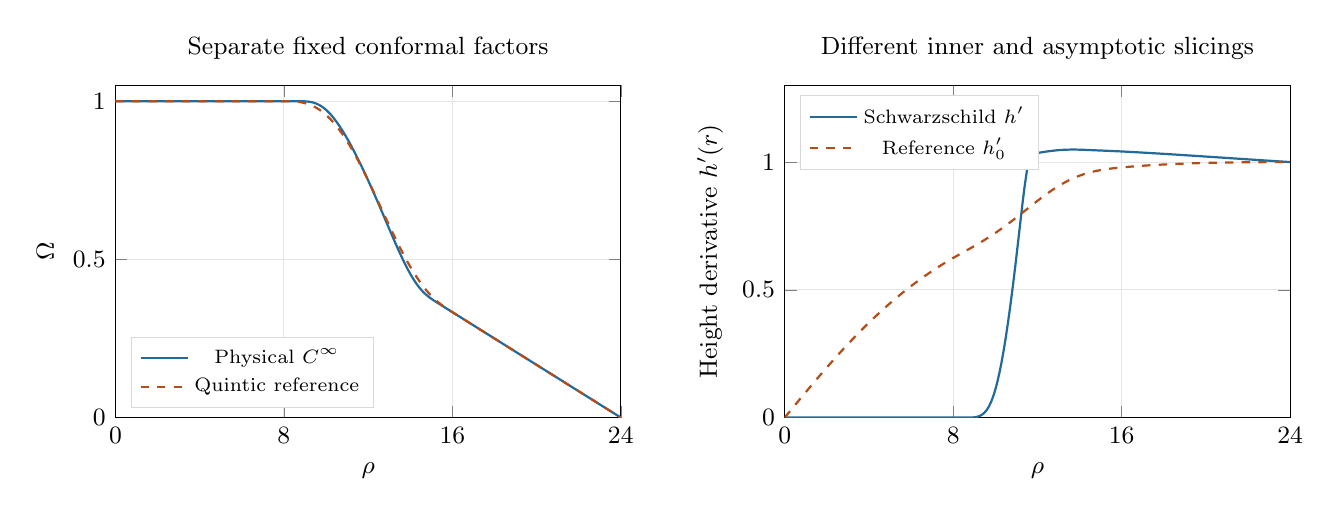
\begin{tikzpicture}
\begin{axis}[width=8cm,height=5.8cm,xmin=0,xmax=24,xtick={0,8,16,24},ymin=0,ymax=1.05,xlabel={$\rho$},ylabel={$\Omega$},title={Separate fixed conformal factors},legend pos=south west]
\addplot[blue,thick] coordinates {(0,1) (0.1,1) (0.2,1) (0.3,1) (0.4,1) (0.5,1) (0.6,1) (0.7,1) (0.8,1) (0.9,1) (1,1) (1.1,1) (1.2,1) (1.3,1) (1.4,1) (1.5,1) (1.6,1) (1.7,1) (1.8,1) (1.9,1) (2,1) (2.1,1) (2.2,1) (2.3,1) (2.4,1) (2.5,1) (2.6,1) (2.7,1) (2.8,1) (2.9,1) (3,1) (3.1,1) (3.2,1) (3.3,1) (3.4,1) (3.5,1) (3.6,1) (3.7,1) (3.8,1) (3.9,1) (4,1) (4.1,1) (4.2,1) (4.3,1) (4.4,1) (4.5,1) (4.6,1) (4.7,1) (4.8,1) (4.9,1) (5,1) (5.1,1) (5.2,1) (5.3,1) (5.4,1) (5.5,1) (5.6,1) (5.7,1) (5.8,1) (5.9,1) (6,1) (6.1,1) (6.2,1) (6.3,1) (6.4,1) (6.5,1) (6.6,1) (6.7,1) (6.8,1) (6.9,1) (7,1) (7.1,1) (7.2,1) (7.3,1) (7.4,1) (7.5,1) (7.6,1) (7.7,1) (7.8,1) (7.9,1) (8,1) (8.1,1) (8.2,1) (8.3,0.999999999997) (8.4,0.999999997933) (8.5,0.999999884191) (8.6,0.999998289199) (8.7,0.999988200393) (8.8,0.999949438943) (8.9,0.999842259036) (9,0.999605946343) (9.1,0.999162674081) (9.2,0.998424472224) (9.3,0.99730092313) (9.4,0.99570598305) (9.5,0.993563183755) (9.6,0.990809052036) (9.7,0.987394897748) (9.8,0.983287254705) (9.9,0.978467293696) (10,0.972929512863) (10.1,0.966679974431) (10.2,0.959734311493) (10.3,0.952115681352) (10.4,0.943852796593) (10.5,0.934978124221) (10.6,0.925526308282) (10.7,0.915532843126) (10.8,0.905033002893) (10.9,0.894061017465) (11,0.882649475191) (11.1,0.87082892718) (11.2,0.858627665851) (11.3,0.846071650751) (11.4,0.833184556643) (11.5,0.819987921757) (11.6,0.806501377474) (11.7,0.792742944124) (11.8,0.778729380812) (11.9,0.764476580006) (12,0.75) (12.1,0.735315130134) (12.2,0.72043798481) (12.3,0.705385622844) (12.4,0.690176688447) (12.5,0.674831969104) (12.6,0.65937496371) (12.7,0.643832451516) (12.8,0.628235048552) (12.9,0.612617733278) (13,0.597020317199) (13.1,0.581487829163) (13.2,0.566070774242) (13.3,0.550825219915) (13.4,0.53581265431) (13.5,0.521099554573) (13.6,0.506756599326) (13.7,0.492857459431) (13.8,0.479477107981) (13.9,0.466689606147) (14,0.454565348658) (14.1,0.443167793827) (14.2,0.432549760189) (14.3,0.422749446275) (14.4,0.413786421946) (14.5,0.405657947603) (14.6,0.398336097248) (14.7,0.391766282795) (14.8,0.385867878017) (14.9,0.380537672842) (15,0.375656756095) (15.1,0.371100961261) (15.2,0.366753999402) (15.3,0.362520751032) (15.4,0.358336396861) (15.5,0.354166877848) (15.6,0.350000003839) (15.7,0.345833333338) (15.8,0.341666666667) (15.9,0.3375) (16,0.333333333333) (16.1,0.329166666667) (16.2,0.325) (16.3,0.320833333333) (16.4,0.316666666667) (16.5,0.3125) (16.6,0.308333333333) (16.7,0.304166666667) (16.8,0.3) (16.9,0.295833333333) (17,0.291666666667) (17.1,0.2875) (17.2,0.283333333333) (17.3,0.279166666667) (17.4,0.275) (17.5,0.270833333333) (17.6,0.266666666667) (17.7,0.2625) (17.8,0.258333333333) (17.9,0.254166666667) (18,0.25) (18.1,0.245833333333) (18.2,0.241666666667) (18.3,0.2375) (18.4,0.233333333333) (18.5,0.229166666667) (18.6,0.225) (18.7,0.220833333333) (18.8,0.216666666667) (18.9,0.2125) (19,0.208333333333) (19.1,0.204166666667) (19.2,0.2) (19.3,0.195833333333) (19.4,0.191666666667) (19.5,0.1875) (19.6,0.183333333333) (19.7,0.179166666667) (19.8,0.175) (19.9,0.170833333333) (20,0.166666666667) (20.1,0.1625) (20.2,0.158333333333) (20.3,0.154166666667) (20.4,0.15) (20.5,0.145833333333) (20.6,0.141666666667) (20.7,0.1375) (20.8,0.133333333333) (20.9,0.129166666667) (21,0.125) (21.1,0.120833333333) (21.2,0.116666666667) (21.3,0.1125) (21.4,0.108333333333) (21.5,0.104166666667) (21.6,0.1) (21.7,0.0958333333333) (21.8,0.0916666666667) (21.9,0.0875) (22,0.0833333333333) (22.1,0.0791666666667) (22.2,0.075) (22.3,0.0708333333333) (22.4,0.0666666666667) (22.5,0.0625) (22.6,0.0583333333333) (22.7,0.0541666666667) (22.8,0.05) (22.9,0.0458333333333) (23,0.0416666666667) (23.1,0.0375) (23.2,0.0333333333333) (23.3,0.0291666666667) (23.4,0.025) (23.5,0.0208333333333) (23.6,0.0166666666667) (23.7,0.0125) (23.8,0.00833333333333) (23.9,0.00416666666667) (24,0)};
\addlegendentry{Physical $C^\infty$}
\addplot[bad,dashed,thick] coordinates {(0,1) (0.1,1) (0.2,1) (0.3,1) (0.4,1) (0.5,1) (0.6,1) (0.7,1) (0.8,1) (0.9,1) (1,1) (1.1,1) (1.2,1) (1.3,1) (1.4,1) (1.5,1) (1.6,1) (1.7,1) (1.8,1) (1.9,1) (2,1) (2.1,1) (2.2,1) (2.3,1) (2.4,1) (2.5,1) (2.6,1) (2.7,1) (2.8,1) (2.9,1) (3,1) (3.1,1) (3.2,1) (3.3,1) (3.4,1) (3.5,1) (3.6,1) (3.7,1) (3.8,1) (3.9,1) (4,1) (4.1,1) (4.2,1) (4.3,1) (4.4,1) (4.5,1) (4.6,1) (4.7,1) (4.8,1) (4.9,1) (5,1) (5.1,1) (5.2,1) (5.3,1) (5.4,1) (5.5,1) (5.6,1) (5.7,1) (5.8,1) (5.9,1) (6,1) (6.1,1) (6.2,1) (6.3,1) (6.4,1) (6.5,1) (6.6,1) (6.7,1) (6.8,1) (6.9,1) (7,1) (7.1,1) (7.2,1) (7.3,1) (7.4,1) (7.5,1) (7.6,1) (7.7,1) (7.8,1) (7.9,1) (8,1) (8.1,0.999993531181) (8.2,0.999948596517) (8.3,0.99982773156) (8.4,0.99959465625) (8.5,0.999214371045) (8.6,0.998653247559) (8.7,0.997879113701) (8.8,0.996861333333) (8.9,0.995570880424) (9,0.993980407715) (9.1,0.992064309888) (9.2,0.98979878125) (9.3,0.987161867912) (9.4,0.984133514486) (9.5,0.980695605278) (9.6,0.976832) (9.7,0.972528563978) (9.8,0.967773192871) (9.9,0.962555831902) (10,0.956868489583) (10.1,0.950705245964) (10.2,0.944062255371) (10.3,0.936937743665) (10.4,0.929332) (10.5,0.921247363091) (10.6,0.912688201986) (10.7,0.90366089135) (10.8,0.89417378125) (10.9,0.884237161451) (11,0.873863220215) (11.1,0.863065997612) (11.2,0.851861333333) (11.3,0.840266809013) (11.4,0.828301685059) (11.5,0.815986831983) (11.6,0.80334465625) (11.7,0.790399020622) (11.8,0.777175159017) (11.9,0.763699585869) (12,0.75) (12.1,0.736105182996) (12.2,0.72204489209) (12.3,0.707849747551) (12.4,0.693551114583) (12.5,0.679180979729) (12.6,0.664771821777) (12.7,0.650356477186) (12.8,0.635968) (12.9,0.621639516289) (13,0.607404073079) (13.1,0.593294481804) (13.2,0.57934315625) (13.3,0.56558194502) (13.4,0.552041958496) (13.5,0.538753390312) (13.6,0.525745333333) (13.7,0.513045590141) (13.8,0.500680478027) (13.9,0.488674628492) (14,0.47705078125) (14.1,0.465829572746) (14.2,0.455029319173) (14.3,0.444665793999) (14.4,0.434752) (14.5,0.425297935804) (14.6,0.416310356934) (14.7,0.407792531364) (14.8,0.399743989583) (14.9,0.392160269157) (15,0.385032653809) (15.1,0.378347906995) (15.2,0.372088) (15.3,0.366229834526) (15.4,0.360744959798) (15.5,0.355599284172) (15.6,0.35075278125) (15.7,0.346159190503) (15.8,0.341765712402) (15.9,0.337512698051) (16,0.333333333333) (16.1,0.329166666667) (16.2,0.325) (16.3,0.320833333333) (16.4,0.316666666667) (16.5,0.3125) (16.6,0.308333333333) (16.7,0.304166666667) (16.8,0.3) (16.9,0.295833333333) (17,0.291666666667) (17.1,0.2875) (17.2,0.283333333333) (17.3,0.279166666667) (17.4,0.275) (17.5,0.270833333333) (17.6,0.266666666667) (17.7,0.2625) (17.8,0.258333333333) (17.9,0.254166666667) (18,0.25) (18.1,0.245833333333) (18.2,0.241666666667) (18.3,0.2375) (18.4,0.233333333333) (18.5,0.229166666667) (18.6,0.225) (18.7,0.220833333333) (18.8,0.216666666667) (18.9,0.2125) (19,0.208333333333) (19.1,0.204166666667) (19.2,0.2) (19.3,0.195833333333) (19.4,0.191666666667) (19.5,0.1875) (19.6,0.183333333333) (19.7,0.179166666667) (19.8,0.175) (19.9,0.170833333333) (20,0.166666666667) (20.1,0.1625) (20.2,0.158333333333) (20.3,0.154166666667) (20.4,0.15) (20.5,0.145833333333) (20.6,0.141666666667) (20.7,0.1375) (20.8,0.133333333333) (20.9,0.129166666667) (21,0.125) (21.1,0.120833333333) (21.2,0.116666666667) (21.3,0.1125) (21.4,0.108333333333) (21.5,0.104166666667) (21.6,0.1) (21.7,0.0958333333333) (21.8,0.0916666666667) (21.9,0.0875) (22,0.0833333333333) (22.1,0.0791666666667) (22.2,0.075) (22.3,0.0708333333333) (22.4,0.0666666666667) (22.5,0.0625) (22.6,0.0583333333333) (22.7,0.0541666666667) (22.8,0.05) (22.9,0.0458333333333) (23,0.0416666666667) (23.1,0.0375) (23.2,0.0333333333333) (23.3,0.0291666666667) (23.4,0.025) (23.5,0.0208333333333) (23.6,0.0166666666667) (23.7,0.0125) (23.8,0.00833333333333) (23.9,0.00416666666667) (24,0)};
\addlegendentry{Quintic reference}
\end{axis}
\begin{axis}[at={(8.5cm,0)},anchor=south west,width=8cm,height=5.8cm,xmin=0,xmax=24,xtick={0,8,16,24},ymin=0,ymax=1.3,xlabel={$\rho$},ylabel={Height derivative $h^\prime(r)$},title={Different inner and asymptotic slicings},legend pos=north west]
\addplot[blue,thick] coordinates {(0,0) (0.1,0) (0.2,0) (0.3,0) (0.4,0) (0.5,0) (0.6,0) (0.7,0) (0.8,0) (0.9,0) (1,0) (1.1,0) (1.2,0) (1.3,0) (1.4,0) (1.5,0) (1.6,0) (1.7,0) (1.8,0) (1.9,0) (2,0) (2.1,0) (2.2,0) (2.3,0) (2.4,0) (2.5,0) (2.6,0) (2.7,0) (2.8,0) (2.9,0) (3,0) (3.1,0) (3.2,0) (3.3,0) (3.4,0) (3.5,0) (3.6,0) (3.7,0) (3.8,0) (3.9,0) (4,0) (4.1,0) (4.2,0) (4.3,0) (4.4,0) (4.5,0) (4.6,0) (4.7,0) (4.8,0) (4.9,0) (5,0) (5.1,0) (5.2,0) (5.3,0) (5.4,0) (5.5,0) (5.6,0) (5.7,0) (5.8,0) (5.9,0) (6,0) (6.1,0) (6.2,0) (6.3,0) (6.4,0) (6.5,0) (6.6,0) (6.7,0) (6.8,0) (6.9,0) (7,0) (7.1,0) (7.2,0) (7.3,0) (7.4,0) (7.5,0) (7.6,0) (7.7,0) (7.8,0) (7.9,0) (8,0) (8.1,4.96755900195e-35) (8.2,1.18473704979e-17) (8.3,7.41444919205e-12) (8.4,5.90756166257e-09) (8.5,3.27193991824e-07) (8.6,4.78008707852e-06) (8.7,3.26446452512e-05) (8.8,0.000138885236516) (8.9,0.000432217690579) (9,0.00108404805811) (9.1,0.00233081210642) (9.2,0.00447496360286) (9.3,0.0078863800438) (9.4,0.0130019265116) (9.5,0.0203191138599) (9.6,0.0303802504994) (9.7,0.0437455238615) (9.8,0.0609563981209) (9.9,0.0824938674779) (10,0.108738561616) (10.1,0.139940532651) (10.2,0.17620519043) (10.3,0.217498442754) (10.4,0.263669539985) (10.5,0.314485682463) (10.6,0.369669114559) (10.7,0.42892540049) (10.8,0.491950132588) (10.9,0.558399124983) (11,0.627802953293) (11.1,0.69940082053) (11.2,0.771866551989) (11.3,0.842920031157) (11.4,0.908909089444) (11.5,0.964697949913) (11.6,1.00465773053) (11.7,1.02581494996) (11.8,1.03236429926) (11.9,1.03407192667) (12,1.03549830401) (12.1,1.03688635199) (12.2,1.03822900459) (12.3,1.03951920854) (12.4,1.04074999228) (12.5,1.04191451991) (12.6,1.04300616213) (12.7,1.04401858687) (12.8,1.04494587137) (12.9,1.0457826366) (13,1.04652420333) (13.1,1.0471667671) (13.2,1.04770758691) (13.3,1.04814517922) (13.4,1.04847950548) (13.5,1.04871213801) (13.6,1.04884638574) (13.7,1.04888735926) (13.8,1.04884195407) (13.9,1.04871873284) (14,1.04852769255) (14.1,1.04827991084) (14.2,1.04798707793) (14.3,1.04766093477) (14.4,1.04731265361) (14.5,1.04695221192) (14.6,1.04658782137) (14.7,1.04622547946) (14.8,1.04586871036) (14.9,1.0455185527) (15,1.04517383469) (15.1,1.04483174557) (15.2,1.04448865706) (15.3,1.0441410569) (15.4,1.04378634215) (15.5,1.04342316769) (15.6,1.04305121796) (15.7,1.0426706728) (15.8,1.04228182692) (15.9,1.04188497877) (16,1.04148041974) (16.1,1.04106843404) (16.2,1.04064929881) (16.3,1.04022328424) (16.4,1.03979065363) (16.5,1.03935166357) (16.6,1.03890656405) (16.7,1.03845559852) (16.8,1.03799900408) (16.9,1.03753701156) (17,1.03706984565) (17.1,1.03659772504) (17.2,1.03612086252) (17.3,1.03563946511) (17.4,1.03515373417) (17.5,1.03466386555) (17.6,1.03417004968) (17.7,1.03367247171) (17.8,1.03317131162) (17.9,1.03266674434) (18,1.03215893984) (18.1,1.03164806331) (18.2,1.03113427518) (18.3,1.03061773133) (18.4,1.03009858313) (18.5,1.02957697757) (18.6,1.02905305736) (18.7,1.02852696108) (18.8,1.0279988232) (18.9,1.02746877425) (19,1.0269369409) (19.1,1.02640344603) (19.2,1.02586840889) (19.3,1.02533194512) (19.4,1.02479416688) (19.5,1.02425518295) (19.6,1.02371509879) (19.7,1.02317401664) (19.8,1.02263203563) (19.9,1.0220892518) (20,1.02154575824) (20.1,1.02100164515) (20.2,1.0204569999) (20.3,1.01991190714) (20.4,1.01936644882) (20.5,1.01882070433) (20.6,1.01827475052) (20.7,1.01772866179) (20.8,1.01718251015) (20.9,1.01663636527) (21,1.01609029459) (21.1,1.01554436333) (21.2,1.01499863459) (21.3,1.01445316937) (21.4,1.01390802667) (21.5,1.01336326351) (21.6,1.01281893502) (21.7,1.01227509445) (21.8,1.01173179326) (21.9,1.01118908117) (22,1.01064700615) (22.1,1.01010561457) (22.2,1.00956495115) (22.3,1.00902505906) (22.4,1.00848597995) (22.5,1.00794775399) (22.6,1.00741041992) (22.7,1.00687401508) (22.8,1.00633857546) (22.9,1.00580413574) (23,1.00527072931) (23.1,1.00473838833) (23.2,1.00420714374) (23.3,1.00367702532) (23.4,1.00314806172) (23.5,1.00262028047) (23.6,1.00209370804) (23.7,1.00156836985) (23.8,1.00104429032) (23.9,1.00052149288) (24,1)};
\addlegendentry{Schwarzschild $h^\prime$}
\addplot[bad,dashed,thick] coordinates {(0,0) (0.1,0.0099995000375) (0.2,0.0199960011996) (0.3,0.0299865091057) (0.4,0.0399680383489) (0.5,0.0499376169439) (0.6,0.0598922907279) (0.7,0.0698291276999) (0.8,0.0797452222829) (0.9,0.0896376994959) (1,0.099503719021) (1.1,0.109340479153) (1.2,0.119145220618) (1.3,0.128915230255) (1.4,0.138647844534) (1.5,0.14834045293) (1.6,0.157990501107) (1.7,0.167595493934) (1.8,0.177152998315) (1.9,0.186660645823) (2,0.196116135138) (2.1,0.205517234286) (2.2,0.214861782675) (2.3,0.224147692921) (2.4,0.233372952475) (2.5,0.242535625036) (2.6,0.251633851765) (2.7,0.260665852291) (2.8,0.26962992552) (2.9,0.278524450246) (3,0.287347885566) (3.1,0.296098771114) (3.2,0.304775727104) (3.3,0.313377454204) (3.4,0.321902733239) (3.5,0.330350424728) (3.6,0.338719468273) (3.7,0.347008881792) (3.8,0.355217760624) (3.9,0.363345276492) (4,0.371390676354) (4.1,0.379353281135) (4.2,0.387232484355) (4.3,0.395027750659) (4.4,0.402738614266) (4.5,0.410364677329) (4.6,0.417905608232) (4.7,0.425361139822) (4.8,0.432731067585) (4.9,0.440015247773) (5,0.4472135955) (5.1,0.454326082796) (5.2,0.461352736642) (5.3,0.468293636984) (5.4,0.475148914735) (5.5,0.481918749772) (5.6,0.488603368932) (5.7,0.49520304401) (5.8,0.501718089772) (5.9,0.508148861978) (6,0.514495755428) (6.1,0.520759202022) (6.2,0.526939668862) (6.3,0.533037656365) (6.4,0.539053696423) (6.5,0.544988350595) (6.6,0.550842208331) (6.7,0.556615885241) (6.8,0.562310021407) (6.9,0.567925279738) (7,0.573462344363) (7.1,0.57892191908) (7.2,0.584304725845) (7.3,0.58961150331) (7.4,0.59484300541) (7.5,0.6) (7.6,0.605083267534) (7.7,0.610093599798) (7.8,0.615031798694) (7.9,0.619898675061) (8,0.624695047554) (8.1,0.629424200132) (8.2,0.634099077901) (8.3,0.638734572169) (8.4,0.643344967516) (8.5,0.647943897353) (8.6,0.65254430668) (8.7,0.657158420918) (8.8,0.661797719773) (8.9,0.666472915191) (9,0.671193932545) (9.1,0.675969894299) (9.2,0.680809105493) (9.3,0.685719040515) (9.4,0.690706330695) (9.5,0.695776752401) (9.6,0.700935215387) (9.7,0.706185751279) (9.8,0.711531502157) (9.9,0.71697470933) (10,0.722516702467) (10.1,0.728157889384) (10.2,0.733897746866) (10.3,0.73973481299) (10.4,0.745666681543) (10.5,0.751689999162) (10.6,0.757800465936) (10.7,0.763992840257) (10.8,0.770260948731) (10.9,0.776597702031) (11,0.782995117512) (11.1,0.789444349446) (11.2,0.795935727616) (11.3,0.802458804963) (11.4,0.809002414831) (11.5,0.815554738173) (11.6,0.822103380919) (11.7,0.828635461428) (11.8,0.835137707698) (11.9,0.841596563714) (12,0.847998304005) (12.1,0.854329155147) (12.2,0.86057542268) (12.3,0.866723621584) (12.4,0.872760608225) (12.5,0.878673711485) (12.6,0.884450860641) (12.7,0.890080707499) (12.8,0.895552740311) (12.9,0.900857387113) (13,0.905986106314) (13.1,0.910931462641) (13.2,0.915687186935) (13.3,0.920248218661) (13.4,0.924610730527) (13.5,0.928772135043) (13.6,0.932731073416) (13.7,0.936487387603) (13.8,0.940042076874) (13.9,0.943397240571) (14,0.946556009155) (14.1,0.949522465831) (14.2,0.952301561285) (14.3,0.954899024095) (14.4,0.95732126941) (14.5,0.959575308408) (14.6,0.961668660866) (14.7,0.963609272952) (14.8,0.965405442065) (14.9,0.967065750183) (15,0.968599006834) (15.1,0.970014202355) (15.2,0.971320471679) (15.3,0.97252706845) (15.4,0.973643348766) (15.5,0.974678763391) (15.6,0.975642856773) (15.7,0.976545270711) (15.8,0.97739574998) (15.9,0.978204146715) (16,0.978980419738) (16.1,0.979733030313) (16.2,0.980464113629) (16.3,0.981174204481) (16.4,0.981863824358) (16.5,0.982533481756) (16.6,0.983183672483) (16.7,0.983814879958) (16.8,0.984427575508) (16.9,0.985022218659) (17,0.985599257417) (17.1,0.986159128553) (17.2,0.986702257871) (17.3,0.987229060482) (17.4,0.987739941063) (17.5,0.988235294118) (17.6,0.988715504225) (17.7,0.989180946289) (17.8,0.989631985782) (17.9,0.990068978976) (18,0.990492273178) (18.1,0.990902206953) (18.2,0.991299110347) (18.3,0.991683305103) (18.4,0.992055104868) (18.5,0.992414815403) (18.6,0.992762734783) (18.7,0.993099153591) (18.8,0.993424355112) (18.9,0.993738615519) (19,0.994042204053) (19.1,0.994335383206) (19.2,0.994618408891) (19.3,0.994891530609) (19.4,0.995154991621) (19.5,0.9954090291) (19.6,0.995653874297) (19.7,0.995889752685) (19.8,0.996116884115) (19.9,0.996335482957) (20,0.996545758245) (20.1,0.99674791381) (20.2,0.99694214842) (20.3,0.997128655905) (20.4,0.99730762529) (20.5,0.997479240916) (20.6,0.997643682562) (20.7,0.99780112556) (20.8,0.997951740916) (20.9,0.998095695415) (21,0.998233151735) (21.1,0.998364268548) (21.2,0.998489200628) (21.3,0.998608098948) (21.4,0.998721110781) (21.5,0.998828379791) (21.6,0.99893004613) (21.7,0.999026246524) (21.8,0.999117114366) (21.9,0.999202779796) (22,0.999283369789) (22.1,0.999359008234) (22.2,0.999429816012) (22.3,0.999495911074) (22.4,0.999557408517) (22.5,0.999614420653) (22.6,0.999667057084) (22.7,0.99971542477) (22.8,0.999759628093) (22.9,0.999799768928) (23,0.999835946701) (23.1,0.999868258455) (23.2,0.999896798908) (23.3,0.999921660513) (23.4,0.999942933514) (23.5,0.999960706003) (23.6,0.999975063973) (23.7,0.999986091372) (23.8,0.999993870153) (23.9,0.999998480325) (24,1)};
\addlegendentry{Reference $h_0^\prime$}
\end{axis}
\end{tikzpicture}\end{center}

\captionof{figure}{Physical and reference compactification factors, and their distinct height derivatives, evaluated from the stated formulas. The physical black-hole height retains the inner trumpet chart and supplies its required asymptotic logarithm. The reference remains the original quintic Minkowski construction. Curves illustrate the selected maps, not an evolving gauge.}

\subsection{Exact conformal pullback and the scri limit}
For $Z^a=(T_{\rm tr},x^i)$ and $z^\mu=(t,y^i)$ the full inverse is
\begin{equation}\label{eq:pullback}
 \G^{\mu\nu}=\Omega^{-2}
 \frac{\partial z^\mu}{\partial Z^a}\frac{\partial z^\nu}{\partial Z^b}g_{\rm tr}^{ab},
 \qquad \frac{\partial t}{\partial x^i}=-h'n_i,
\end{equation}
\begin{equation}
 \frac{\partial y^i}{\partial x^j}
 =\Omega(\delta^i{}_j-n^in_j)+\frac{\Omega^2}{\lambda}n^in_j.
\end{equation}
The implementation factors the nominally cancelling $\Omega^2$ analytically, retaining all higher-order mass and spin terms. It evaluates $\Omega=0$ directly, without a large-radius cutoff. Define
\begin{equation}
 \bar\Sigma=(\rho+M\Omega)^2+a^2\Omega^2n_z^2,\quad
 D=\sqrt{-\G}=\frac{\lambda\bar\Sigma}{\rho^2},\quad
 C_{\rm eff}^{,2}=C^2+4M(M+c)-a^2(1-n_z^2).
\end{equation}
At $\rho=S$, the regular limits are
\begin{equation}\label{eq:scrilimit}
 \G^{tt}=-\frac{C_{\rm eff}^{,2}}{S^2},\qquad
 \G^{ti}=-n^i,\qquad \G^{ij}=\delta^{ij}-n^in^j,\qquad D=1.
\end{equation}
The inverse spacetime metric is regular there; only its radial spatial block becomes characteristic. Spacelike time slices require $\G^{tt}<0$, which is checked on the actual geometry.

\clearpage
\section{Scalar equation and conformal curvature}
\subsection{Physical equation and exact rescaling}
The physical target is
\begin{equation}\label{eq:physical}
 \Box_g\Phi=\frac{1}{\sqrt{-g}}\partial_a\!\left(\sqrt{-g}\,g^{ab}\partial_b\Phi\right)=0.
\end{equation}
In four spacetime dimensions the conformal identity is
\begin{equation}\label{eq:confid}
 \left(\Box_{\G}-\frac{R[\G]}{6}\right)\psi
 =\Omega^{-3}\left(\Box_g-\frac{R[g]}{6}\right)(\Omega\psi).
\end{equation}
Every physical background here is vacuum, so $R[g]=0$. Consequently
\begin{equation}\label{eq:conformal}
 (\Box_{\G}-V)\psi=0,\qquad
 V=\frac{R[\G]}6=-\Omega^{-3}\Box_g\Omega.
\end{equation}
The physical scalar is minimally coupled and massless. The curvature term in the rescaled equation is forced by the transformation; it is not an added physical scalar mass. This is the same conformal identity used for fixed-background scalar evolution in \cite{matching}.

For the exact trumpet, $\Delta=R^2-2MR+a^2=r^2-c^2$. A radial $\Omega$ gives
\begin{align}
 \Box_g\Omega&=\frac1\Sigma\partial_r(\Delta\partial_r\Omega),\\
 V&=-\frac{\Omega}{\lambda\bar\Sigma}\partial_\rho
 \left[\frac{(\rho^2-c^2\Omega^2)\Omega'}{\lambda}\right],
 \qquad V|_{\scri}=0.
\end{align}
The radial-azimuthal flux has zero azimuthal divergence. The height transformation does not change this stationary scalar contraction. Crucially, $R[\G]$ is the curvature of the \emph{actual conformal physical metric}, not $R[\bar\eta_{\rm ref}]$.

\subsection{Frozen wave-operator coefficients}
Stationarity allows the equation to be written
\begin{equation}\label{eq:expanded}
 \G^{tt}\psi_{tt}+2\G^{ti}\psi_{ti}+\G^{ij}\psi_{ij}
 +B^t\psi_t+B^i\psi_i-V\psi=0,\qquad
 B^\mu=\frac1D\partial_i(D\G^{i\mu}).
\end{equation}
All $\G^{\mu\nu},B^\mu,D,V$ and required lapse/shift derivatives are cached before evolution. First spatial coefficient derivatives use analytic jets. Independent value-only, high-precision pullbacks check the cached coefficients, their derivatives and the curvature identity.

The current endpoint audit has scaled error about $2.1\times10^{-16}$; the corrected critical conformal-curvature probes agree to about $1.95\times10^{-18}$. A separate million-point Minkowski check agrees within $4.33\times10^{-15}$. These are coefficient checks, not substitutes for field convergence.

\clearpage
\section{First-order scalar evolution systems}
\subsection{Current normal-momentum system}
From the conformal physical inverse define
\begin{equation}
 \alpha=(-\G^{tt})^{-1/2},\qquad \beta^i=-\frac{\G^{ti}}{\G^{tt}},\qquad
 \gamma^{ij}=\G^{ij}-\frac{\G^{ti}\G^{tj}}{\G^{tt}},
\end{equation}
The defining derivative equalities below hold on the scalar reduction surface. Numerical deviations are measured, rather than reset to zero.
\begin{equation}
 q_i=\partial_i\psi,\qquad \Pi=-n^\mu\partial_\mu\psi
 =\frac{\beta^iq_i-\partial_t\psi}{\alpha},\qquad C_i=q_i-\partial_i\psi.
\end{equation}
Here $\alpha,\beta,\gamma,K$ belong to $\G$, not to the untransformed physical trumpet decomposition. With $K_{ij}=-(1/2)\mathcal L_n\gamma_{ij}$ and $\Gamma^i=\gamma^{jk}{}^{(3)}\Gamma^i{}_{jk}$,
\begin{align}\label{eq:normal}
 \partial_t\psi&=\beta^i\partial_i\psi-\alpha\Pi,\\
 \partial_t\Pi&=\beta^i\partial_i\Pi-\alpha\gamma^{ij}\partial_iq_j
 +\alpha K\Pi+(\alpha\Gamma^j-\gamma^{ij}\partial_i\alpha)q_j+\alpha V\psi,\\
 \partial_tq_i&=\beta^j\partial_jq_i-\alpha\partial_i\Pi
 +(\partial_i\beta^j)q_j-(\partial_i\alpha)\Pi-\kappa C_i.
\end{align}
The current configuration has $\kappa=0$. A nonzero $\kappa$ is scalar auxiliary feedback computed from the derived reduction residual; it introduces no extra evolved field. Its diagnostic trial is discussed below.

The code obtains the stationary source coefficients from the same frozen wave operator:
\begin{align}
 s_\Pi&=\alpha^2B^t+\frac{\beta^i\partial_i\alpha}{\alpha}=\alpha K,\\
 s_q^{,i}&=-\alpha(B^t\beta^i+B^i)
 -\frac{\beta^j\partial_j\beta^i}{\alpha}
 =\alpha\Gamma^i-\gamma^{ji}\partial_j\alpha.
\end{align}
Thus the symbols $K$ and $\Gamma^i$ describe fixed coefficients, not gravitational evolution variables.

\subsection{Reduction and derivative diagnostics}
At the continuum level the derived residual obeys
\begin{equation}
 \partial_t C_i=\beta^j\partial_jC_i+(\partial_i\beta^j)C_j-\kappa C_i.
\end{equation}
This equation explains the reduction; it is not separately integrated. The measured residual is $C_i^h=q_i-D_i^c\psi$. Snapshots contain the independent centred gradient and
\begin{equation}
 v_{\rm rec}=\beta^iD_i^c\psi-\alpha\Pi,
 \qquad (\psi_t)_h=\beta^iD_i^{\rm up}\psi-\alpha\Pi.
\end{equation}
These differ at truncation order. Both the reconstruction and the actual compiled scalar RHS are checked. Calling the evolved $q_i$ an exact derivative would miss reduction error.

\clearpage
\subsection{Earlier coordinate-velocity reduction}
The earlier five-field form uses $v=\partial_t\psi$ and $q_i=\partial_i\psi$:
\begin{align}
 \psi_t&=v,\\
 v_t&=-\frac{2\G^{ti}\partial_iv+\G^{ij}\partial_iq_j+B^tv+B^iq_i-V\psi}{\G^{tt}},\\
 (q_i)_t&=\partial_iv+\beta^j(\partial_jq_i-\partial_iq_j).
\end{align}
The curl term vanishes on the reduction surface and transports reduction modes. Its damped variant changes $\psi_t$ to $v-\beta^iC_i$, adds $-\kappa C_i$ to $q_{i,t}$ and $-\kappa\beta^iC_i$ to $v_t$. In that variant $v$ is an auxiliary off the reduction surface; the physical coordinate derivative is $v-\beta\cdot C$. These historical settings are not the current undamped normal-momentum configuration.

\subsection{Actual characteristics and the outer boundary}
For any spatial covector $m_i$, set $\beta^m=\beta^im_i$ and $s_m^2=\gamma^{ij}m_im_j$. The principal scalar speeds and fields are
\begin{equation}
 c_\pm=-\beta^m\pm\alpha s_m,\qquad c_0=-\beta^m,\qquad
 U_\pm=\Pi\pm\frac{\gamma^{ij}m_iq_j}{s_m}.
\end{equation}
Equivalently, with $b=\G^{ti}m_i/\G^{tt}$,
\begin{equation}
 c_\pm=b\pm\sqrt{b^2-\frac{\G^{ij}m_im_j}{\G^{tt}}}.
\end{equation}
At exact scri and outward radial $m=n$, equation~\eqref{eq:scrilimit} gives
\begin{equation}
 c_-=0,\qquad c_+=\frac{2S^2}{C_{\rm eff}^{,2}}.
\end{equation}
No incoming boundary data are prescribed at scri. Logical-coordinate speeds include the map Jacobian; their signs, rather than unscaled magnitudes, identify inflow and outflow.

At a finite cap there is an incoming mode. The implemented asymptotic scalar penalty uses
\begin{align}
 \delta&=\Pi-q_n-\frac{c_+}{\alpha}A_\rho\psi,\qquad
 q_n=\frac{\gamma^{ij}n_iq_j}{\sqrt{\gamma^{ij}n_in_j}},\qquad
 A_\rho=\frac{1+M\Omega'}{\rho+M\Omega},\\
 \Pi_t&\longmapsto\Pi_t-\tfrac12\sigma\delta,\qquad
 q_{i,t}\longmapsto q_{i,t}+\tfrac12\sigma\frac{n_i}{s_n}\delta.
\end{align}
Here $\sigma\geq0$ is the mapped incoming speed divided by the radial norm weight and grid spacing. This is an asymptotic finite-radius condition, not exact black-hole radiation data. Boundary sensitivity must be measured. Analytic incoming ghosts are restricted to flat-space verification controls.

\clearpage
\section{Computational domain and patch maps}
\begin{center}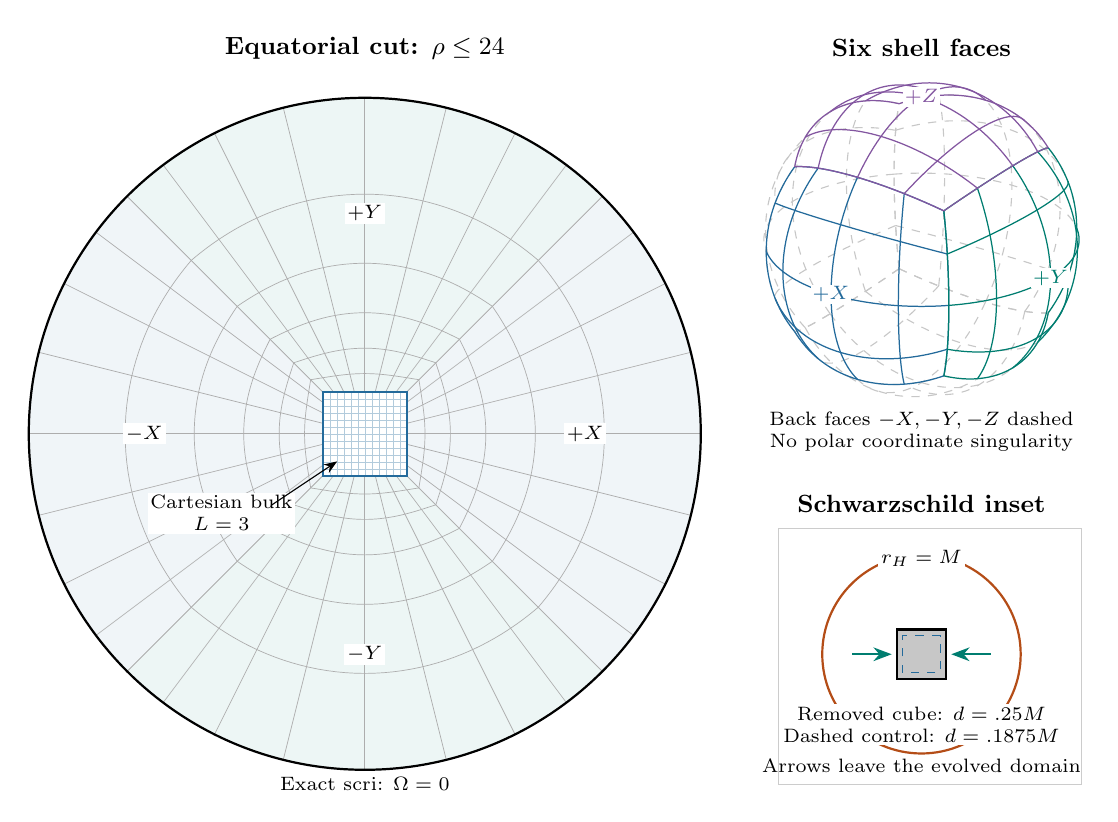
\begin{tikzpicture}[x=1.4cm,y=1.4cm,font=\scriptsize]
\node[font=\small\bfseries] at (0,3.5) {Equatorial cut: $\rho\leq24$};
\fill[blue!7] (0.38100,-0.38100) -- (0.38100,-0.34290) -- (0.38100,-0.30480) -- (0.38100,-0.26670) -- (0.38100,-0.22860) -- (0.38100,-0.19050) -- (0.38100,-0.15240) -- (0.38100,-0.11430) -- (0.38100,-0.07620) -- (0.38100,-0.03810) -- (0.38100,0.00000) -- (0.38100,0.03810) -- (0.38100,0.07620) -- (0.38100,0.11430) -- (0.38100,0.15240) -- (0.38100,0.19050) -- (0.38100,0.22860) -- (0.38100,0.26670) -- (0.38100,0.30480) -- (0.38100,0.34290) -- (0.38100,0.38100) -- (2.15526,2.15526) -- (2.20980,2.09931) -- (2.26556,2.03900) -- (2.32239,1.97403) -- (2.38009,1.90407) -- (2.43840,1.82880) -- (2.49702,1.74791) -- (2.55558,1.66112) -- (2.61364,1.56818) -- (2.67071,1.46889) -- (2.72621,1.36311) -- (2.77954,1.25079) -- (2.83000,1.13200) -- (2.87688,1.00691) -- (2.91945,0.87584) -- (2.95699,0.73925) -- (2.98881,0.59776) -- (3.01428,0.45214) -- (3.03287,0.30329) -- (3.04420,0.15221) -- (3.04800,0.00000) -- (3.04420,-0.15221) -- (3.03287,-0.30329) -- (3.01428,-0.45214) -- (2.98881,-0.59776) -- (2.95699,-0.73925) -- (2.91945,-0.87584) -- (2.87688,-1.00691) -- (2.83000,-1.13200) -- (2.77954,-1.25079) -- (2.72621,-1.36311) -- (2.67071,-1.46889) -- (2.61364,-1.56818) -- (2.55558,-1.66112) -- (2.49702,-1.74791) -- (2.43840,-1.82880) -- (2.38009,-1.90407) -- (2.32239,-1.97403) -- (2.26556,-2.03900) -- (2.20980,-2.09931) -- (2.15526,-2.15526) -- cycle;
\draw[black!32,line width=.25pt] (0.38100,-0.38100) -- (0.38100,-0.36576) -- (0.38100,-0.35052) -- (0.38100,-0.33528) -- (0.38100,-0.32004) -- (0.38100,-0.30480) -- (0.38100,-0.28956) -- (0.38100,-0.27432) -- (0.38100,-0.25908) -- (0.38100,-0.24384) -- (0.38100,-0.22860) -- (0.38100,-0.21336) -- (0.38100,-0.19812) -- (0.38100,-0.18288) -- (0.38100,-0.16764) -- (0.38100,-0.15240) -- (0.38100,-0.13716) -- (0.38100,-0.12192) -- (0.38100,-0.10668) -- (0.38100,-0.09144) -- (0.38100,-0.07620) -- (0.38100,-0.06096) -- (0.38100,-0.04572) -- (0.38100,-0.03048) -- (0.38100,-0.01524) -- (0.38100,0.00000) -- (0.38100,0.01524) -- (0.38100,0.03048) -- (0.38100,0.04572) -- (0.38100,0.06096) -- (0.38100,0.07620) -- (0.38100,0.09144) -- (0.38100,0.10668) -- (0.38100,0.12192) -- (0.38100,0.13716) -- (0.38100,0.15240) -- (0.38100,0.16764) -- (0.38100,0.18288) -- (0.38100,0.19812) -- (0.38100,0.21336) -- (0.38100,0.22860) -- (0.38100,0.24384) -- (0.38100,0.25908) -- (0.38100,0.27432) -- (0.38100,0.28956) -- (0.38100,0.30480) -- (0.38100,0.32004) -- (0.38100,0.33528) -- (0.38100,0.35052) -- (0.38100,0.36576) -- (0.38100,0.38100);
\draw[black!32,line width=.25pt] (0.49086,-0.49086) -- (0.49356,-0.47382) -- (0.49630,-0.45660) -- (0.49909,-0.43920) -- (0.50192,-0.42161) -- (0.50478,-0.40383) -- (0.50767,-0.38583) -- (0.51057,-0.36761) -- (0.51348,-0.34916) -- (0.51637,-0.33048) -- (0.51925,-0.31155) -- (0.52208,-0.29236) -- (0.52486,-0.27292) -- (0.52756,-0.25323) -- (0.53016,-0.23327) -- (0.53264,-0.21306) -- (0.53498,-0.19259) -- (0.53716,-0.17189) -- (0.53915,-0.15096) -- (0.54093,-0.12982) -- (0.54248,-0.10850) -- (0.54377,-0.08700) -- (0.54480,-0.06538) -- (0.54554,-0.04364) -- (0.54599,-0.02184) -- (0.54614,0.00000) -- (0.54599,0.02184) -- (0.54554,0.04364) -- (0.54480,0.06538) -- (0.54377,0.08700) -- (0.54248,0.10850) -- (0.54093,0.12982) -- (0.53915,0.15096) -- (0.53716,0.17189) -- (0.53498,0.19259) -- (0.53264,0.21306) -- (0.53016,0.23327) -- (0.52756,0.25323) -- (0.52486,0.27292) -- (0.52208,0.29236) -- (0.51925,0.31155) -- (0.51637,0.33048) -- (0.51348,0.34916) -- (0.51057,0.36761) -- (0.50767,0.38583) -- (0.50478,0.40383) -- (0.50192,0.42161) -- (0.49909,0.43920) -- (0.49630,0.45660) -- (0.49356,0.47382) -- (0.49086,0.49086);
\draw[black!32,line width=.25pt] (0.64419,-0.64419) -- (0.65065,-0.62462) -- (0.65722,-0.60464) -- (0.66390,-0.58424) -- (0.67068,-0.56337) -- (0.67754,-0.54203) -- (0.68445,-0.52018) -- (0.69140,-0.49781) -- (0.69836,-0.47489) -- (0.70530,-0.45139) -- (0.71218,-0.42731) -- (0.71897,-0.40262) -- (0.72562,-0.37732) -- (0.73209,-0.35140) -- (0.73833,-0.32486) -- (0.74428,-0.29771) -- (0.74989,-0.26996) -- (0.75510,-0.24163) -- (0.75987,-0.21276) -- (0.76413,-0.18339) -- (0.76783,-0.15357) -- (0.77094,-0.12335) -- (0.77339,-0.09281) -- (0.77518,-0.06201) -- (0.77625,-0.03105) -- (0.77662,0.00000) -- (0.77625,0.03105) -- (0.77518,0.06201) -- (0.77339,0.09281) -- (0.77094,0.12335) -- (0.76783,0.15357) -- (0.76413,0.18339) -- (0.75987,0.21276) -- (0.75510,0.24163) -- (0.74989,0.26996) -- (0.74428,0.29771) -- (0.73833,0.32486) -- (0.73209,0.35140) -- (0.72562,0.37732) -- (0.71897,0.40262) -- (0.71218,0.42731) -- (0.70530,0.45139) -- (0.69836,0.47489) -- (0.69140,0.49781) -- (0.68445,0.52018) -- (0.67754,0.54203) -- (0.67068,0.56337) -- (0.66390,0.58424) -- (0.65722,0.60464) -- (0.65065,0.62462) -- (0.64419,0.64419);
\draw[black!32,line width=.25pt] (0.85817,-0.85817) -- (0.86988,-0.83508) -- (0.88180,-0.81126) -- (0.89392,-0.78665) -- (0.90621,-0.76121) -- (0.91864,-0.73491) -- (0.93117,-0.70769) -- (0.94378,-0.67952) -- (0.95639,-0.65035) -- (0.96897,-0.62014) -- (0.98145,-0.58887) -- (0.99376,-0.55650) -- (1.00581,-0.52302) -- (1.01754,-0.48842) -- (1.02885,-0.45269) -- (1.03964,-0.41585) -- (1.04981,-0.37793) -- (1.05927,-0.33897) -- (1.06791,-0.29901) -- (1.07563,-0.25815) -- (1.08235,-0.21647) -- (1.08797,-0.17408) -- (1.09243,-0.13109) -- (1.09566,-0.08765) -- (1.09761,-0.04390) -- (1.09827,0.00000) -- (1.09761,0.04390) -- (1.09566,0.08765) -- (1.09243,0.13109) -- (1.08797,0.17408) -- (1.08235,0.21647) -- (1.07563,0.25815) -- (1.06791,0.29901) -- (1.05927,0.33897) -- (1.04981,0.37793) -- (1.03964,0.41585) -- (1.02885,0.45269) -- (1.01754,0.48842) -- (1.00581,0.52302) -- (0.99376,0.55650) -- (0.98145,0.58887) -- (0.96897,0.62014) -- (0.95639,0.65035) -- (0.94378,0.67952) -- (0.93117,0.70769) -- (0.91864,0.73491) -- (0.90621,0.76121) -- (0.89392,0.78665) -- (0.88180,0.81126) -- (0.86988,0.83508) -- (0.85817,0.85817);
\draw[black!32,line width=.25pt] (1.15681,-1.15681) -- (1.17584,-1.12881) -- (1.19523,-1.09961) -- (1.21493,-1.06914) -- (1.23491,-1.03732) -- (1.25512,-1.00409) -- (1.27550,-0.96938) -- (1.29599,-0.93311) -- (1.31650,-0.89522) -- (1.33695,-0.85565) -- (1.35724,-0.81434) -- (1.37725,-0.77126) -- (1.39685,-0.72636) -- (1.41592,-0.67964) -- (1.43430,-0.63109) -- (1.45184,-0.58074) -- (1.46838,-0.52862) -- (1.48376,-0.47480) -- (1.49781,-0.41939) -- (1.51037,-0.36249) -- (1.52129,-0.30426) -- (1.53043,-0.24487) -- (1.53767,-0.18452) -- (1.54292,-0.12343) -- (1.54610,-0.06184) -- (1.54717,0.00000) -- (1.54610,0.06184) -- (1.54292,0.12343) -- (1.53767,0.18452) -- (1.53043,0.24487) -- (1.52129,0.30426) -- (1.51037,0.36249) -- (1.49781,0.41939) -- (1.48376,0.47480) -- (1.46838,0.52862) -- (1.45184,0.58074) -- (1.43430,0.63109) -- (1.41592,0.67964) -- (1.39685,0.72636) -- (1.37725,0.77126) -- (1.35724,0.81434) -- (1.33695,0.85565) -- (1.31650,0.89522) -- (1.29599,0.93311) -- (1.27550,0.96938) -- (1.25512,1.00409) -- (1.23491,1.03732) -- (1.21493,1.06914) -- (1.19523,1.09961) -- (1.17584,1.12881) -- (1.15681,1.15681);
\draw[black!32,line width=.25pt] (1.57359,-1.57359) -- (1.60285,-1.53874) -- (1.63265,-1.50204) -- (1.66293,-1.46338) -- (1.69365,-1.42266) -- (1.72471,-1.37977) -- (1.75605,-1.33460) -- (1.78754,-1.28703) -- (1.81907,-1.23697) -- (1.85051,-1.18433) -- (1.88170,-1.12902) -- (1.91246,-1.07098) -- (1.94259,-1.01015) -- (1.97190,-0.94651) -- (2.00016,-0.88007) -- (2.02713,-0.81085) -- (2.05255,-0.73892) -- (2.07619,-0.66438) -- (2.09778,-0.58738) -- (2.11709,-0.50810) -- (2.13387,-0.42677) -- (2.14793,-0.34367) -- (2.15907,-0.25909) -- (2.16714,-0.17337) -- (2.17202,-0.08688) -- (2.17366,0.00000) -- (2.17202,0.08688) -- (2.16714,0.17337) -- (2.15907,0.25909) -- (2.14793,0.34367) -- (2.13387,0.42677) -- (2.11709,0.50810) -- (2.09778,0.58738) -- (2.07619,0.66438) -- (2.05255,0.73892) -- (2.02713,0.81085) -- (2.00016,0.88007) -- (1.97190,0.94651) -- (1.94259,1.01015) -- (1.91246,1.07098) -- (1.88170,1.12902) -- (1.85051,1.18433) -- (1.81907,1.23697) -- (1.78754,1.28703) -- (1.75605,1.33460) -- (1.72471,1.37977) -- (1.69365,1.42266) -- (1.66293,1.46338) -- (1.63265,1.50204) -- (1.60285,1.53874) -- (1.57359,1.57359);
\draw[black!32,line width=.25pt] (2.15526,-2.15526) -- (2.19879,-2.11084) -- (2.24312,-2.06367) -- (2.28817,-2.01359) -- (2.33387,-1.96045) -- (2.38009,-1.90407) -- (2.42670,-1.84429) -- (2.47356,-1.78096) -- (2.52047,-1.71392) -- (2.56724,-1.64304) -- (2.61364,-1.56818) -- (2.65940,-1.48926) -- (2.70424,-1.40620) -- (2.74784,-1.31896) -- (2.78988,-1.22755) -- (2.83000,-1.13200) -- (2.86782,-1.03242) -- (2.90299,-0.92896) -- (2.93511,-0.82183) -- (2.96384,-0.71132) -- (2.98881,-0.59776) -- (3.00972,-0.48156) -- (3.02629,-0.36315) -- (3.03829,-0.24306) -- (3.04556,-0.12182) -- (3.04800,0.00000) -- (3.04556,0.12182) -- (3.03829,0.24306) -- (3.02629,0.36315) -- (3.00972,0.48156) -- (2.98881,0.59776) -- (2.96384,0.71132) -- (2.93511,0.82183) -- (2.90299,0.92896) -- (2.86782,1.03242) -- (2.83000,1.13200) -- (2.78988,1.22755) -- (2.74784,1.31896) -- (2.70424,1.40620) -- (2.65940,1.48926) -- (2.61364,1.56818) -- (2.56724,1.64304) -- (2.52047,1.71392) -- (2.47356,1.78096) -- (2.42670,1.84429) -- (2.38009,1.90407) -- (2.33387,1.96045) -- (2.28817,2.01359) -- (2.24312,2.06367) -- (2.19879,2.11084) -- (2.15526,2.15526);
\draw[black!32,line width=.25pt] (0.38100,-0.38100) -- (0.40014,-0.40014) -- (0.42061,-0.42061) -- (0.44248,-0.44248) -- (0.46587,-0.46587) -- (0.49086,-0.49086) -- (0.51758,-0.51758) -- (0.54614,-0.54614) -- (0.57667,-0.57667) -- (0.60931,-0.60931) -- (0.64419,-0.64419) -- (0.68148,-0.68148) -- (0.72134,-0.72134) -- (0.76394,-0.76394) -- (0.80949,-0.80949) -- (0.85817,-0.85817) -- (0.91021,-0.91021) -- (0.96584,-0.96584) -- (1.02530,-1.02530) -- (1.08887,-1.08887) -- (1.15681,-1.15681) -- (1.22944,-1.22944) -- (1.30707,-1.30707) -- (1.39006,-1.39006) -- (1.47877,-1.47877) -- (1.57359,-1.57359) -- (1.67495,-1.67495) -- (1.78330,-1.78330) -- (1.89912,-1.89912) -- (2.02292,-2.02292) -- (2.15526,-2.15526);
\draw[black!32,line width=.25pt] (0.38100,-0.28575) -- (0.40320,-0.30240) -- (0.42693,-0.32020) -- (0.45230,-0.33922) -- (0.47941,-0.35956) -- (0.50839,-0.38130) -- (0.53938,-0.40453) -- (0.57250,-0.42937) -- (0.60790,-0.45592) -- (0.64574,-0.48430) -- (0.68619,-0.51464) -- (0.72943,-0.54707) -- (0.77565,-0.58174) -- (0.82505,-0.61879) -- (0.87787,-0.65840) -- (0.93432,-0.70074) -- (0.99467,-0.74600) -- (1.05917,-0.79438) -- (1.12812,-0.84609) -- (1.20183,-0.90137) -- (1.28062,-0.96046) -- (1.36483,-1.02363) -- (1.45486,-1.09114) -- (1.55109,-1.16332) -- (1.65395,-1.24046) -- (1.76391,-1.32293) -- (1.88145,-1.41108) -- (2.00708,-1.50531) -- (2.14138,-1.60604) -- (2.28494,-1.71371) -- (2.43840,-1.82880);
\draw[black!32,line width=.25pt] (0.38100,-0.19050) -- (0.40631,-0.20315) -- (0.43336,-0.21668) -- (0.46227,-0.23113) -- (0.49318,-0.24659) -- (0.52622,-0.26311) -- (0.56153,-0.28077) -- (0.59928,-0.29964) -- (0.63964,-0.31982) -- (0.68277,-0.34139) -- (0.72888,-0.36444) -- (0.77817,-0.38909) -- (0.83086,-0.41543) -- (0.88717,-0.44359) -- (0.94737,-0.47369) -- (1.01173,-0.50586) -- (1.08051,-0.54026) -- (1.15404,-0.57702) -- (1.23264,-0.61632) -- (1.31666,-0.65833) -- (1.40646,-0.70323) -- (1.50246,-0.75123) -- (1.60508,-0.80254) -- (1.71477,-0.85739) -- (1.83203,-0.91601) -- (1.95737,-0.97868) -- (2.09135,-1.04567) -- (2.23456,-1.11728) -- (2.38765,-1.19382) -- (2.55129,-1.27565) -- (2.72621,-1.36311);
\draw[black!32,line width=.25pt] (0.38100,-0.09525) -- (0.40880,-0.10220) -- (0.43851,-0.10963) -- (0.47027,-0.11757) -- (0.50422,-0.12605) -- (0.54051,-0.13513) -- (0.57930,-0.14482) -- (0.62076,-0.15519) -- (0.66509,-0.16627) -- (0.71247,-0.17812) -- (0.76312,-0.19078) -- (0.81725,-0.20431) -- (0.87512,-0.21878) -- (0.93698,-0.23425) -- (1.00311,-0.25078) -- (1.07379,-0.26845) -- (1.14935,-0.28734) -- (1.23011,-0.30753) -- (1.31644,-0.32911) -- (1.40873,-0.35218) -- (1.50737,-0.37684) -- (1.61282,-0.40321) -- (1.72554,-0.43138) -- (1.84602,-0.46151) -- (1.97482,-0.49370) -- (2.11249,-0.52812) -- (2.25965,-0.56491) -- (2.41696,-0.60424) -- (2.58511,-0.64628) -- (2.76486,-0.69121) -- (2.95699,-0.73925);
\draw[black!32,line width=.25pt] (0.38100,0.00000) -- (0.40978,0.00000) -- (0.44054,0.00000) -- (0.47342,0.00000) -- (0.50857,0.00000) -- (0.54614,0.00000) -- (0.58630,0.00000) -- (0.62923,0.00000) -- (0.67513,0.00000) -- (0.72418,0.00000) -- (0.77662,0.00000) -- (0.83267,0.00000) -- (0.89258,0.00000) -- (0.95663,0.00000) -- (1.02509,0.00000) -- (1.09827,0.00000) -- (1.17649,0.00000) -- (1.26011,0.00000) -- (1.34949,0.00000) -- (1.44504,0.00000) -- (1.54717,0.00000) -- (1.65634,0.00000) -- (1.77304,0.00000) -- (1.89778,0.00000) -- (2.03112,0.00000) -- (2.17366,0.00000) -- (2.32602,0.00000) -- (2.48889,0.00000) -- (2.66298,0.00000) -- (2.84908,0.00000) -- (3.04800,0.00000);
\draw[black!32,line width=.25pt] (0.38100,0.09525) -- (0.40880,0.10220) -- (0.43851,0.10963) -- (0.47027,0.11757) -- (0.50422,0.12605) -- (0.54051,0.13513) -- (0.57930,0.14482) -- (0.62076,0.15519) -- (0.66509,0.16627) -- (0.71247,0.17812) -- (0.76312,0.19078) -- (0.81725,0.20431) -- (0.87512,0.21878) -- (0.93698,0.23425) -- (1.00311,0.25078) -- (1.07379,0.26845) -- (1.14935,0.28734) -- (1.23011,0.30753) -- (1.31644,0.32911) -- (1.40873,0.35218) -- (1.50737,0.37684) -- (1.61282,0.40321) -- (1.72554,0.43138) -- (1.84602,0.46151) -- (1.97482,0.49370) -- (2.11249,0.52812) -- (2.25965,0.56491) -- (2.41696,0.60424) -- (2.58511,0.64628) -- (2.76486,0.69121) -- (2.95699,0.73925);
\draw[black!32,line width=.25pt] (0.38100,0.19050) -- (0.40631,0.20315) -- (0.43336,0.21668) -- (0.46227,0.23113) -- (0.49318,0.24659) -- (0.52622,0.26311) -- (0.56153,0.28077) -- (0.59928,0.29964) -- (0.63964,0.31982) -- (0.68277,0.34139) -- (0.72888,0.36444) -- (0.77817,0.38909) -- (0.83086,0.41543) -- (0.88717,0.44359) -- (0.94737,0.47369) -- (1.01173,0.50586) -- (1.08051,0.54026) -- (1.15404,0.57702) -- (1.23264,0.61632) -- (1.31666,0.65833) -- (1.40646,0.70323) -- (1.50246,0.75123) -- (1.60508,0.80254) -- (1.71477,0.85739) -- (1.83203,0.91601) -- (1.95737,0.97868) -- (2.09135,1.04567) -- (2.23456,1.11728) -- (2.38765,1.19382) -- (2.55129,1.27565) -- (2.72621,1.36311);
\draw[black!32,line width=.25pt] (0.38100,0.28575) -- (0.40320,0.30240) -- (0.42693,0.32020) -- (0.45230,0.33922) -- (0.47941,0.35956) -- (0.50839,0.38130) -- (0.53938,0.40453) -- (0.57250,0.42937) -- (0.60790,0.45592) -- (0.64574,0.48430) -- (0.68619,0.51464) -- (0.72943,0.54707) -- (0.77565,0.58174) -- (0.82505,0.61879) -- (0.87787,0.65840) -- (0.93432,0.70074) -- (0.99467,0.74600) -- (1.05917,0.79438) -- (1.12812,0.84609) -- (1.20183,0.90137) -- (1.28062,0.96046) -- (1.36483,1.02363) -- (1.45486,1.09114) -- (1.55109,1.16332) -- (1.65395,1.24046) -- (1.76391,1.32293) -- (1.88145,1.41108) -- (2.00708,1.50531) -- (2.14138,1.60604) -- (2.28494,1.71371) -- (2.43840,1.82880);
\draw[black!32,line width=.25pt] (0.38100,0.38100) -- (0.40014,0.40014) -- (0.42061,0.42061) -- (0.44248,0.44248) -- (0.46587,0.46587) -- (0.49086,0.49086) -- (0.51758,0.51758) -- (0.54614,0.54614) -- (0.57667,0.57667) -- (0.60931,0.60931) -- (0.64419,0.64419) -- (0.68148,0.68148) -- (0.72134,0.72134) -- (0.76394,0.76394) -- (0.80949,0.80949) -- (0.85817,0.85817) -- (0.91021,0.91021) -- (0.96584,0.96584) -- (1.02530,1.02530) -- (1.08887,1.08887) -- (1.15681,1.15681) -- (1.22944,1.22944) -- (1.30707,1.30707) -- (1.39006,1.39006) -- (1.47877,1.47877) -- (1.57359,1.57359) -- (1.67495,1.67495) -- (1.78330,1.78330) -- (1.89912,1.89912) -- (2.02292,2.02292) -- (2.15526,2.15526);
\fill[blue!7] (-0.38100,-0.38100) -- (-0.38100,-0.34290) -- (-0.38100,-0.30480) -- (-0.38100,-0.26670) -- (-0.38100,-0.22860) -- (-0.38100,-0.19050) -- (-0.38100,-0.15240) -- (-0.38100,-0.11430) -- (-0.38100,-0.07620) -- (-0.38100,-0.03810) -- (-0.38100,0.00000) -- (-0.38100,0.03810) -- (-0.38100,0.07620) -- (-0.38100,0.11430) -- (-0.38100,0.15240) -- (-0.38100,0.19050) -- (-0.38100,0.22860) -- (-0.38100,0.26670) -- (-0.38100,0.30480) -- (-0.38100,0.34290) -- (-0.38100,0.38100) -- (-2.15526,2.15526) -- (-2.20980,2.09931) -- (-2.26556,2.03900) -- (-2.32239,1.97403) -- (-2.38009,1.90407) -- (-2.43840,1.82880) -- (-2.49702,1.74791) -- (-2.55558,1.66112) -- (-2.61364,1.56818) -- (-2.67071,1.46889) -- (-2.72621,1.36311) -- (-2.77954,1.25079) -- (-2.83000,1.13200) -- (-2.87688,1.00691) -- (-2.91945,0.87584) -- (-2.95699,0.73925) -- (-2.98881,0.59776) -- (-3.01428,0.45214) -- (-3.03287,0.30329) -- (-3.04420,0.15221) -- (-3.04800,0.00000) -- (-3.04420,-0.15221) -- (-3.03287,-0.30329) -- (-3.01428,-0.45214) -- (-2.98881,-0.59776) -- (-2.95699,-0.73925) -- (-2.91945,-0.87584) -- (-2.87688,-1.00691) -- (-2.83000,-1.13200) -- (-2.77954,-1.25079) -- (-2.72621,-1.36311) -- (-2.67071,-1.46889) -- (-2.61364,-1.56818) -- (-2.55558,-1.66112) -- (-2.49702,-1.74791) -- (-2.43840,-1.82880) -- (-2.38009,-1.90407) -- (-2.32239,-1.97403) -- (-2.26556,-2.03900) -- (-2.20980,-2.09931) -- (-2.15526,-2.15526) -- cycle;
\draw[black!32,line width=.25pt] (-0.38100,-0.38100) -- (-0.38100,-0.36576) -- (-0.38100,-0.35052) -- (-0.38100,-0.33528) -- (-0.38100,-0.32004) -- (-0.38100,-0.30480) -- (-0.38100,-0.28956) -- (-0.38100,-0.27432) -- (-0.38100,-0.25908) -- (-0.38100,-0.24384) -- (-0.38100,-0.22860) -- (-0.38100,-0.21336) -- (-0.38100,-0.19812) -- (-0.38100,-0.18288) -- (-0.38100,-0.16764) -- (-0.38100,-0.15240) -- (-0.38100,-0.13716) -- (-0.38100,-0.12192) -- (-0.38100,-0.10668) -- (-0.38100,-0.09144) -- (-0.38100,-0.07620) -- (-0.38100,-0.06096) -- (-0.38100,-0.04572) -- (-0.38100,-0.03048) -- (-0.38100,-0.01524) -- (-0.38100,0.00000) -- (-0.38100,0.01524) -- (-0.38100,0.03048) -- (-0.38100,0.04572) -- (-0.38100,0.06096) -- (-0.38100,0.07620) -- (-0.38100,0.09144) -- (-0.38100,0.10668) -- (-0.38100,0.12192) -- (-0.38100,0.13716) -- (-0.38100,0.15240) -- (-0.38100,0.16764) -- (-0.38100,0.18288) -- (-0.38100,0.19812) -- (-0.38100,0.21336) -- (-0.38100,0.22860) -- (-0.38100,0.24384) -- (-0.38100,0.25908) -- (-0.38100,0.27432) -- (-0.38100,0.28956) -- (-0.38100,0.30480) -- (-0.38100,0.32004) -- (-0.38100,0.33528) -- (-0.38100,0.35052) -- (-0.38100,0.36576) -- (-0.38100,0.38100);
\draw[black!32,line width=.25pt] (-0.49086,-0.49086) -- (-0.49356,-0.47382) -- (-0.49630,-0.45660) -- (-0.49909,-0.43920) -- (-0.50192,-0.42161) -- (-0.50478,-0.40383) -- (-0.50767,-0.38583) -- (-0.51057,-0.36761) -- (-0.51348,-0.34916) -- (-0.51637,-0.33048) -- (-0.51925,-0.31155) -- (-0.52208,-0.29236) -- (-0.52486,-0.27292) -- (-0.52756,-0.25323) -- (-0.53016,-0.23327) -- (-0.53264,-0.21306) -- (-0.53498,-0.19259) -- (-0.53716,-0.17189) -- (-0.53915,-0.15096) -- (-0.54093,-0.12982) -- (-0.54248,-0.10850) -- (-0.54377,-0.08700) -- (-0.54480,-0.06538) -- (-0.54554,-0.04364) -- (-0.54599,-0.02184) -- (-0.54614,0.00000) -- (-0.54599,0.02184) -- (-0.54554,0.04364) -- (-0.54480,0.06538) -- (-0.54377,0.08700) -- (-0.54248,0.10850) -- (-0.54093,0.12982) -- (-0.53915,0.15096) -- (-0.53716,0.17189) -- (-0.53498,0.19259) -- (-0.53264,0.21306) -- (-0.53016,0.23327) -- (-0.52756,0.25323) -- (-0.52486,0.27292) -- (-0.52208,0.29236) -- (-0.51925,0.31155) -- (-0.51637,0.33048) -- (-0.51348,0.34916) -- (-0.51057,0.36761) -- (-0.50767,0.38583) -- (-0.50478,0.40383) -- (-0.50192,0.42161) -- (-0.49909,0.43920) -- (-0.49630,0.45660) -- (-0.49356,0.47382) -- (-0.49086,0.49086);
\draw[black!32,line width=.25pt] (-0.64419,-0.64419) -- (-0.65065,-0.62462) -- (-0.65722,-0.60464) -- (-0.66390,-0.58424) -- (-0.67068,-0.56337) -- (-0.67754,-0.54203) -- (-0.68445,-0.52018) -- (-0.69140,-0.49781) -- (-0.69836,-0.47489) -- (-0.70530,-0.45139) -- (-0.71218,-0.42731) -- (-0.71897,-0.40262) -- (-0.72562,-0.37732) -- (-0.73209,-0.35140) -- (-0.73833,-0.32486) -- (-0.74428,-0.29771) -- (-0.74989,-0.26996) -- (-0.75510,-0.24163) -- (-0.75987,-0.21276) -- (-0.76413,-0.18339) -- (-0.76783,-0.15357) -- (-0.77094,-0.12335) -- (-0.77339,-0.09281) -- (-0.77518,-0.06201) -- (-0.77625,-0.03105) -- (-0.77662,0.00000) -- (-0.77625,0.03105) -- (-0.77518,0.06201) -- (-0.77339,0.09281) -- (-0.77094,0.12335) -- (-0.76783,0.15357) -- (-0.76413,0.18339) -- (-0.75987,0.21276) -- (-0.75510,0.24163) -- (-0.74989,0.26996) -- (-0.74428,0.29771) -- (-0.73833,0.32486) -- (-0.73209,0.35140) -- (-0.72562,0.37732) -- (-0.71897,0.40262) -- (-0.71218,0.42731) -- (-0.70530,0.45139) -- (-0.69836,0.47489) -- (-0.69140,0.49781) -- (-0.68445,0.52018) -- (-0.67754,0.54203) -- (-0.67068,0.56337) -- (-0.66390,0.58424) -- (-0.65722,0.60464) -- (-0.65065,0.62462) -- (-0.64419,0.64419);
\draw[black!32,line width=.25pt] (-0.85817,-0.85817) -- (-0.86988,-0.83508) -- (-0.88180,-0.81126) -- (-0.89392,-0.78665) -- (-0.90621,-0.76121) -- (-0.91864,-0.73491) -- (-0.93117,-0.70769) -- (-0.94378,-0.67952) -- (-0.95639,-0.65035) -- (-0.96897,-0.62014) -- (-0.98145,-0.58887) -- (-0.99376,-0.55650) -- (-1.00581,-0.52302) -- (-1.01754,-0.48842) -- (-1.02885,-0.45269) -- (-1.03964,-0.41585) -- (-1.04981,-0.37793) -- (-1.05927,-0.33897) -- (-1.06791,-0.29901) -- (-1.07563,-0.25815) -- (-1.08235,-0.21647) -- (-1.08797,-0.17408) -- (-1.09243,-0.13109) -- (-1.09566,-0.08765) -- (-1.09761,-0.04390) -- (-1.09827,0.00000) -- (-1.09761,0.04390) -- (-1.09566,0.08765) -- (-1.09243,0.13109) -- (-1.08797,0.17408) -- (-1.08235,0.21647) -- (-1.07563,0.25815) -- (-1.06791,0.29901) -- (-1.05927,0.33897) -- (-1.04981,0.37793) -- (-1.03964,0.41585) -- (-1.02885,0.45269) -- (-1.01754,0.48842) -- (-1.00581,0.52302) -- (-0.99376,0.55650) -- (-0.98145,0.58887) -- (-0.96897,0.62014) -- (-0.95639,0.65035) -- (-0.94378,0.67952) -- (-0.93117,0.70769) -- (-0.91864,0.73491) -- (-0.90621,0.76121) -- (-0.89392,0.78665) -- (-0.88180,0.81126) -- (-0.86988,0.83508) -- (-0.85817,0.85817);
\draw[black!32,line width=.25pt] (-1.15681,-1.15681) -- (-1.17584,-1.12881) -- (-1.19523,-1.09961) -- (-1.21493,-1.06914) -- (-1.23491,-1.03732) -- (-1.25512,-1.00409) -- (-1.27550,-0.96938) -- (-1.29599,-0.93311) -- (-1.31650,-0.89522) -- (-1.33695,-0.85565) -- (-1.35724,-0.81434) -- (-1.37725,-0.77126) -- (-1.39685,-0.72636) -- (-1.41592,-0.67964) -- (-1.43430,-0.63109) -- (-1.45184,-0.58074) -- (-1.46838,-0.52862) -- (-1.48376,-0.47480) -- (-1.49781,-0.41939) -- (-1.51037,-0.36249) -- (-1.52129,-0.30426) -- (-1.53043,-0.24487) -- (-1.53767,-0.18452) -- (-1.54292,-0.12343) -- (-1.54610,-0.06184) -- (-1.54717,0.00000) -- (-1.54610,0.06184) -- (-1.54292,0.12343) -- (-1.53767,0.18452) -- (-1.53043,0.24487) -- (-1.52129,0.30426) -- (-1.51037,0.36249) -- (-1.49781,0.41939) -- (-1.48376,0.47480) -- (-1.46838,0.52862) -- (-1.45184,0.58074) -- (-1.43430,0.63109) -- (-1.41592,0.67964) -- (-1.39685,0.72636) -- (-1.37725,0.77126) -- (-1.35724,0.81434) -- (-1.33695,0.85565) -- (-1.31650,0.89522) -- (-1.29599,0.93311) -- (-1.27550,0.96938) -- (-1.25512,1.00409) -- (-1.23491,1.03732) -- (-1.21493,1.06914) -- (-1.19523,1.09961) -- (-1.17584,1.12881) -- (-1.15681,1.15681);
\draw[black!32,line width=.25pt] (-1.57359,-1.57359) -- (-1.60285,-1.53874) -- (-1.63265,-1.50204) -- (-1.66293,-1.46338) -- (-1.69365,-1.42266) -- (-1.72471,-1.37977) -- (-1.75605,-1.33460) -- (-1.78754,-1.28703) -- (-1.81907,-1.23697) -- (-1.85051,-1.18433) -- (-1.88170,-1.12902) -- (-1.91246,-1.07098) -- (-1.94259,-1.01015) -- (-1.97190,-0.94651) -- (-2.00016,-0.88007) -- (-2.02713,-0.81085) -- (-2.05255,-0.73892) -- (-2.07619,-0.66438) -- (-2.09778,-0.58738) -- (-2.11709,-0.50810) -- (-2.13387,-0.42677) -- (-2.14793,-0.34367) -- (-2.15907,-0.25909) -- (-2.16714,-0.17337) -- (-2.17202,-0.08688) -- (-2.17366,0.00000) -- (-2.17202,0.08688) -- (-2.16714,0.17337) -- (-2.15907,0.25909) -- (-2.14793,0.34367) -- (-2.13387,0.42677) -- (-2.11709,0.50810) -- (-2.09778,0.58738) -- (-2.07619,0.66438) -- (-2.05255,0.73892) -- (-2.02713,0.81085) -- (-2.00016,0.88007) -- (-1.97190,0.94651) -- (-1.94259,1.01015) -- (-1.91246,1.07098) -- (-1.88170,1.12902) -- (-1.85051,1.18433) -- (-1.81907,1.23697) -- (-1.78754,1.28703) -- (-1.75605,1.33460) -- (-1.72471,1.37977) -- (-1.69365,1.42266) -- (-1.66293,1.46338) -- (-1.63265,1.50204) -- (-1.60285,1.53874) -- (-1.57359,1.57359);
\draw[black!32,line width=.25pt] (-2.15526,-2.15526) -- (-2.19879,-2.11084) -- (-2.24312,-2.06367) -- (-2.28817,-2.01359) -- (-2.33387,-1.96045) -- (-2.38009,-1.90407) -- (-2.42670,-1.84429) -- (-2.47356,-1.78096) -- (-2.52047,-1.71392) -- (-2.56724,-1.64304) -- (-2.61364,-1.56818) -- (-2.65940,-1.48926) -- (-2.70424,-1.40620) -- (-2.74784,-1.31896) -- (-2.78988,-1.22755) -- (-2.83000,-1.13200) -- (-2.86782,-1.03242) -- (-2.90299,-0.92896) -- (-2.93511,-0.82183) -- (-2.96384,-0.71132) -- (-2.98881,-0.59776) -- (-3.00972,-0.48156) -- (-3.02629,-0.36315) -- (-3.03829,-0.24306) -- (-3.04556,-0.12182) -- (-3.04800,0.00000) -- (-3.04556,0.12182) -- (-3.03829,0.24306) -- (-3.02629,0.36315) -- (-3.00972,0.48156) -- (-2.98881,0.59776) -- (-2.96384,0.71132) -- (-2.93511,0.82183) -- (-2.90299,0.92896) -- (-2.86782,1.03242) -- (-2.83000,1.13200) -- (-2.78988,1.22755) -- (-2.74784,1.31896) -- (-2.70424,1.40620) -- (-2.65940,1.48926) -- (-2.61364,1.56818) -- (-2.56724,1.64304) -- (-2.52047,1.71392) -- (-2.47356,1.78096) -- (-2.42670,1.84429) -- (-2.38009,1.90407) -- (-2.33387,1.96045) -- (-2.28817,2.01359) -- (-2.24312,2.06367) -- (-2.19879,2.11084) -- (-2.15526,2.15526);
\draw[black!32,line width=.25pt] (-0.38100,-0.38100) -- (-0.40014,-0.40014) -- (-0.42061,-0.42061) -- (-0.44248,-0.44248) -- (-0.46587,-0.46587) -- (-0.49086,-0.49086) -- (-0.51758,-0.51758) -- (-0.54614,-0.54614) -- (-0.57667,-0.57667) -- (-0.60931,-0.60931) -- (-0.64419,-0.64419) -- (-0.68148,-0.68148) -- (-0.72134,-0.72134) -- (-0.76394,-0.76394) -- (-0.80949,-0.80949) -- (-0.85817,-0.85817) -- (-0.91021,-0.91021) -- (-0.96584,-0.96584) -- (-1.02530,-1.02530) -- (-1.08887,-1.08887) -- (-1.15681,-1.15681) -- (-1.22944,-1.22944) -- (-1.30707,-1.30707) -- (-1.39006,-1.39006) -- (-1.47877,-1.47877) -- (-1.57359,-1.57359) -- (-1.67495,-1.67495) -- (-1.78330,-1.78330) -- (-1.89912,-1.89912) -- (-2.02292,-2.02292) -- (-2.15526,-2.15526);
\draw[black!32,line width=.25pt] (-0.38100,-0.28575) -- (-0.40320,-0.30240) -- (-0.42693,-0.32020) -- (-0.45230,-0.33922) -- (-0.47941,-0.35956) -- (-0.50839,-0.38130) -- (-0.53938,-0.40453) -- (-0.57250,-0.42937) -- (-0.60790,-0.45592) -- (-0.64574,-0.48430) -- (-0.68619,-0.51464) -- (-0.72943,-0.54707) -- (-0.77565,-0.58174) -- (-0.82505,-0.61879) -- (-0.87787,-0.65840) -- (-0.93432,-0.70074) -- (-0.99467,-0.74600) -- (-1.05917,-0.79438) -- (-1.12812,-0.84609) -- (-1.20183,-0.90137) -- (-1.28062,-0.96046) -- (-1.36483,-1.02363) -- (-1.45486,-1.09114) -- (-1.55109,-1.16332) -- (-1.65395,-1.24046) -- (-1.76391,-1.32293) -- (-1.88145,-1.41108) -- (-2.00708,-1.50531) -- (-2.14138,-1.60604) -- (-2.28494,-1.71371) -- (-2.43840,-1.82880);
\draw[black!32,line width=.25pt] (-0.38100,-0.19050) -- (-0.40631,-0.20315) -- (-0.43336,-0.21668) -- (-0.46227,-0.23113) -- (-0.49318,-0.24659) -- (-0.52622,-0.26311) -- (-0.56153,-0.28077) -- (-0.59928,-0.29964) -- (-0.63964,-0.31982) -- (-0.68277,-0.34139) -- (-0.72888,-0.36444) -- (-0.77817,-0.38909) -- (-0.83086,-0.41543) -- (-0.88717,-0.44359) -- (-0.94737,-0.47369) -- (-1.01173,-0.50586) -- (-1.08051,-0.54026) -- (-1.15404,-0.57702) -- (-1.23264,-0.61632) -- (-1.31666,-0.65833) -- (-1.40646,-0.70323) -- (-1.50246,-0.75123) -- (-1.60508,-0.80254) -- (-1.71477,-0.85739) -- (-1.83203,-0.91601) -- (-1.95737,-0.97868) -- (-2.09135,-1.04567) -- (-2.23456,-1.11728) -- (-2.38765,-1.19382) -- (-2.55129,-1.27565) -- (-2.72621,-1.36311);
\draw[black!32,line width=.25pt] (-0.38100,-0.09525) -- (-0.40880,-0.10220) -- (-0.43851,-0.10963) -- (-0.47027,-0.11757) -- (-0.50422,-0.12605) -- (-0.54051,-0.13513) -- (-0.57930,-0.14482) -- (-0.62076,-0.15519) -- (-0.66509,-0.16627) -- (-0.71247,-0.17812) -- (-0.76312,-0.19078) -- (-0.81725,-0.20431) -- (-0.87512,-0.21878) -- (-0.93698,-0.23425) -- (-1.00311,-0.25078) -- (-1.07379,-0.26845) -- (-1.14935,-0.28734) -- (-1.23011,-0.30753) -- (-1.31644,-0.32911) -- (-1.40873,-0.35218) -- (-1.50737,-0.37684) -- (-1.61282,-0.40321) -- (-1.72554,-0.43138) -- (-1.84602,-0.46151) -- (-1.97482,-0.49370) -- (-2.11249,-0.52812) -- (-2.25965,-0.56491) -- (-2.41696,-0.60424) -- (-2.58511,-0.64628) -- (-2.76486,-0.69121) -- (-2.95699,-0.73925);
\draw[black!32,line width=.25pt] (-0.38100,0.00000) -- (-0.40978,0.00000) -- (-0.44054,0.00000) -- (-0.47342,0.00000) -- (-0.50857,0.00000) -- (-0.54614,0.00000) -- (-0.58630,0.00000) -- (-0.62923,0.00000) -- (-0.67513,0.00000) -- (-0.72418,0.00000) -- (-0.77662,0.00000) -- (-0.83267,0.00000) -- (-0.89258,0.00000) -- (-0.95663,0.00000) -- (-1.02509,0.00000) -- (-1.09827,0.00000) -- (-1.17649,0.00000) -- (-1.26011,0.00000) -- (-1.34949,0.00000) -- (-1.44504,0.00000) -- (-1.54717,0.00000) -- (-1.65634,0.00000) -- (-1.77304,0.00000) -- (-1.89778,0.00000) -- (-2.03112,0.00000) -- (-2.17366,0.00000) -- (-2.32602,0.00000) -- (-2.48889,0.00000) -- (-2.66298,0.00000) -- (-2.84908,0.00000) -- (-3.04800,0.00000);
\draw[black!32,line width=.25pt] (-0.38100,0.09525) -- (-0.40880,0.10220) -- (-0.43851,0.10963) -- (-0.47027,0.11757) -- (-0.50422,0.12605) -- (-0.54051,0.13513) -- (-0.57930,0.14482) -- (-0.62076,0.15519) -- (-0.66509,0.16627) -- (-0.71247,0.17812) -- (-0.76312,0.19078) -- (-0.81725,0.20431) -- (-0.87512,0.21878) -- (-0.93698,0.23425) -- (-1.00311,0.25078) -- (-1.07379,0.26845) -- (-1.14935,0.28734) -- (-1.23011,0.30753) -- (-1.31644,0.32911) -- (-1.40873,0.35218) -- (-1.50737,0.37684) -- (-1.61282,0.40321) -- (-1.72554,0.43138) -- (-1.84602,0.46151) -- (-1.97482,0.49370) -- (-2.11249,0.52812) -- (-2.25965,0.56491) -- (-2.41696,0.60424) -- (-2.58511,0.64628) -- (-2.76486,0.69121) -- (-2.95699,0.73925);
\draw[black!32,line width=.25pt] (-0.38100,0.19050) -- (-0.40631,0.20315) -- (-0.43336,0.21668) -- (-0.46227,0.23113) -- (-0.49318,0.24659) -- (-0.52622,0.26311) -- (-0.56153,0.28077) -- (-0.59928,0.29964) -- (-0.63964,0.31982) -- (-0.68277,0.34139) -- (-0.72888,0.36444) -- (-0.77817,0.38909) -- (-0.83086,0.41543) -- (-0.88717,0.44359) -- (-0.94737,0.47369) -- (-1.01173,0.50586) -- (-1.08051,0.54026) -- (-1.15404,0.57702) -- (-1.23264,0.61632) -- (-1.31666,0.65833) -- (-1.40646,0.70323) -- (-1.50246,0.75123) -- (-1.60508,0.80254) -- (-1.71477,0.85739) -- (-1.83203,0.91601) -- (-1.95737,0.97868) -- (-2.09135,1.04567) -- (-2.23456,1.11728) -- (-2.38765,1.19382) -- (-2.55129,1.27565) -- (-2.72621,1.36311);
\draw[black!32,line width=.25pt] (-0.38100,0.28575) -- (-0.40320,0.30240) -- (-0.42693,0.32020) -- (-0.45230,0.33922) -- (-0.47941,0.35956) -- (-0.50839,0.38130) -- (-0.53938,0.40453) -- (-0.57250,0.42937) -- (-0.60790,0.45592) -- (-0.64574,0.48430) -- (-0.68619,0.51464) -- (-0.72943,0.54707) -- (-0.77565,0.58174) -- (-0.82505,0.61879) -- (-0.87787,0.65840) -- (-0.93432,0.70074) -- (-0.99467,0.74600) -- (-1.05917,0.79438) -- (-1.12812,0.84609) -- (-1.20183,0.90137) -- (-1.28062,0.96046) -- (-1.36483,1.02363) -- (-1.45486,1.09114) -- (-1.55109,1.16332) -- (-1.65395,1.24046) -- (-1.76391,1.32293) -- (-1.88145,1.41108) -- (-2.00708,1.50531) -- (-2.14138,1.60604) -- (-2.28494,1.71371) -- (-2.43840,1.82880);
\draw[black!32,line width=.25pt] (-0.38100,0.38100) -- (-0.40014,0.40014) -- (-0.42061,0.42061) -- (-0.44248,0.44248) -- (-0.46587,0.46587) -- (-0.49086,0.49086) -- (-0.51758,0.51758) -- (-0.54614,0.54614) -- (-0.57667,0.57667) -- (-0.60931,0.60931) -- (-0.64419,0.64419) -- (-0.68148,0.68148) -- (-0.72134,0.72134) -- (-0.76394,0.76394) -- (-0.80949,0.80949) -- (-0.85817,0.85817) -- (-0.91021,0.91021) -- (-0.96584,0.96584) -- (-1.02530,1.02530) -- (-1.08887,1.08887) -- (-1.15681,1.15681) -- (-1.22944,1.22944) -- (-1.30707,1.30707) -- (-1.39006,1.39006) -- (-1.47877,1.47877) -- (-1.57359,1.57359) -- (-1.67495,1.67495) -- (-1.78330,1.78330) -- (-1.89912,1.89912) -- (-2.02292,2.02292) -- (-2.15526,2.15526);
\fill[good!7] (-0.38100,0.38100) -- (-0.34290,0.38100) -- (-0.30480,0.38100) -- (-0.26670,0.38100) -- (-0.22860,0.38100) -- (-0.19050,0.38100) -- (-0.15240,0.38100) -- (-0.11430,0.38100) -- (-0.07620,0.38100) -- (-0.03810,0.38100) -- (0.00000,0.38100) -- (0.03810,0.38100) -- (0.07620,0.38100) -- (0.11430,0.38100) -- (0.15240,0.38100) -- (0.19050,0.38100) -- (0.22860,0.38100) -- (0.26670,0.38100) -- (0.30480,0.38100) -- (0.34290,0.38100) -- (0.38100,0.38100) -- (2.15526,2.15526) -- (2.09931,2.20980) -- (2.03900,2.26556) -- (1.97403,2.32239) -- (1.90407,2.38009) -- (1.82880,2.43840) -- (1.74791,2.49702) -- (1.66112,2.55558) -- (1.56818,2.61364) -- (1.46889,2.67071) -- (1.36311,2.72621) -- (1.25079,2.77954) -- (1.13200,2.83000) -- (1.00691,2.87688) -- (0.87584,2.91945) -- (0.73925,2.95699) -- (0.59776,2.98881) -- (0.45214,3.01428) -- (0.30329,3.03287) -- (0.15221,3.04420) -- (0.00000,3.04800) -- (-0.15221,3.04420) -- (-0.30329,3.03287) -- (-0.45214,3.01428) -- (-0.59776,2.98881) -- (-0.73925,2.95699) -- (-0.87584,2.91945) -- (-1.00691,2.87688) -- (-1.13200,2.83000) -- (-1.25079,2.77954) -- (-1.36311,2.72621) -- (-1.46889,2.67071) -- (-1.56818,2.61364) -- (-1.66112,2.55558) -- (-1.74791,2.49702) -- (-1.82880,2.43840) -- (-1.90407,2.38009) -- (-1.97403,2.32239) -- (-2.03900,2.26556) -- (-2.09931,2.20980) -- (-2.15526,2.15526) -- cycle;
\draw[black!32,line width=.25pt] (-0.38100,0.38100) -- (-0.36576,0.38100) -- (-0.35052,0.38100) -- (-0.33528,0.38100) -- (-0.32004,0.38100) -- (-0.30480,0.38100) -- (-0.28956,0.38100) -- (-0.27432,0.38100) -- (-0.25908,0.38100) -- (-0.24384,0.38100) -- (-0.22860,0.38100) -- (-0.21336,0.38100) -- (-0.19812,0.38100) -- (-0.18288,0.38100) -- (-0.16764,0.38100) -- (-0.15240,0.38100) -- (-0.13716,0.38100) -- (-0.12192,0.38100) -- (-0.10668,0.38100) -- (-0.09144,0.38100) -- (-0.07620,0.38100) -- (-0.06096,0.38100) -- (-0.04572,0.38100) -- (-0.03048,0.38100) -- (-0.01524,0.38100) -- (0.00000,0.38100) -- (0.01524,0.38100) -- (0.03048,0.38100) -- (0.04572,0.38100) -- (0.06096,0.38100) -- (0.07620,0.38100) -- (0.09144,0.38100) -- (0.10668,0.38100) -- (0.12192,0.38100) -- (0.13716,0.38100) -- (0.15240,0.38100) -- (0.16764,0.38100) -- (0.18288,0.38100) -- (0.19812,0.38100) -- (0.21336,0.38100) -- (0.22860,0.38100) -- (0.24384,0.38100) -- (0.25908,0.38100) -- (0.27432,0.38100) -- (0.28956,0.38100) -- (0.30480,0.38100) -- (0.32004,0.38100) -- (0.33528,0.38100) -- (0.35052,0.38100) -- (0.36576,0.38100) -- (0.38100,0.38100);
\draw[black!32,line width=.25pt] (-0.49086,0.49086) -- (-0.47382,0.49356) -- (-0.45660,0.49630) -- (-0.43920,0.49909) -- (-0.42161,0.50192) -- (-0.40383,0.50478) -- (-0.38583,0.50767) -- (-0.36761,0.51057) -- (-0.34916,0.51348) -- (-0.33048,0.51637) -- (-0.31155,0.51925) -- (-0.29236,0.52208) -- (-0.27292,0.52486) -- (-0.25323,0.52756) -- (-0.23327,0.53016) -- (-0.21306,0.53264) -- (-0.19259,0.53498) -- (-0.17189,0.53716) -- (-0.15096,0.53915) -- (-0.12982,0.54093) -- (-0.10850,0.54248) -- (-0.08700,0.54377) -- (-0.06538,0.54480) -- (-0.04364,0.54554) -- (-0.02184,0.54599) -- (0.00000,0.54614) -- (0.02184,0.54599) -- (0.04364,0.54554) -- (0.06538,0.54480) -- (0.08700,0.54377) -- (0.10850,0.54248) -- (0.12982,0.54093) -- (0.15096,0.53915) -- (0.17189,0.53716) -- (0.19259,0.53498) -- (0.21306,0.53264) -- (0.23327,0.53016) -- (0.25323,0.52756) -- (0.27292,0.52486) -- (0.29236,0.52208) -- (0.31155,0.51925) -- (0.33048,0.51637) -- (0.34916,0.51348) -- (0.36761,0.51057) -- (0.38583,0.50767) -- (0.40383,0.50478) -- (0.42161,0.50192) -- (0.43920,0.49909) -- (0.45660,0.49630) -- (0.47382,0.49356) -- (0.49086,0.49086);
\draw[black!32,line width=.25pt] (-0.64419,0.64419) -- (-0.62462,0.65065) -- (-0.60464,0.65722) -- (-0.58424,0.66390) -- (-0.56337,0.67068) -- (-0.54203,0.67754) -- (-0.52018,0.68445) -- (-0.49781,0.69140) -- (-0.47489,0.69836) -- (-0.45139,0.70530) -- (-0.42731,0.71218) -- (-0.40262,0.71897) -- (-0.37732,0.72562) -- (-0.35140,0.73209) -- (-0.32486,0.73833) -- (-0.29771,0.74428) -- (-0.26996,0.74989) -- (-0.24163,0.75510) -- (-0.21276,0.75987) -- (-0.18339,0.76413) -- (-0.15357,0.76783) -- (-0.12335,0.77094) -- (-0.09281,0.77339) -- (-0.06201,0.77518) -- (-0.03105,0.77625) -- (0.00000,0.77662) -- (0.03105,0.77625) -- (0.06201,0.77518) -- (0.09281,0.77339) -- (0.12335,0.77094) -- (0.15357,0.76783) -- (0.18339,0.76413) -- (0.21276,0.75987) -- (0.24163,0.75510) -- (0.26996,0.74989) -- (0.29771,0.74428) -- (0.32486,0.73833) -- (0.35140,0.73209) -- (0.37732,0.72562) -- (0.40262,0.71897) -- (0.42731,0.71218) -- (0.45139,0.70530) -- (0.47489,0.69836) -- (0.49781,0.69140) -- (0.52018,0.68445) -- (0.54203,0.67754) -- (0.56337,0.67068) -- (0.58424,0.66390) -- (0.60464,0.65722) -- (0.62462,0.65065) -- (0.64419,0.64419);
\draw[black!32,line width=.25pt] (-0.85817,0.85817) -- (-0.83508,0.86988) -- (-0.81126,0.88180) -- (-0.78665,0.89392) -- (-0.76121,0.90621) -- (-0.73491,0.91864) -- (-0.70769,0.93117) -- (-0.67952,0.94378) -- (-0.65035,0.95639) -- (-0.62014,0.96897) -- (-0.58887,0.98145) -- (-0.55650,0.99376) -- (-0.52302,1.00581) -- (-0.48842,1.01754) -- (-0.45269,1.02885) -- (-0.41585,1.03964) -- (-0.37793,1.04981) -- (-0.33897,1.05927) -- (-0.29901,1.06791) -- (-0.25815,1.07563) -- (-0.21647,1.08235) -- (-0.17408,1.08797) -- (-0.13109,1.09243) -- (-0.08765,1.09566) -- (-0.04390,1.09761) -- (0.00000,1.09827) -- (0.04390,1.09761) -- (0.08765,1.09566) -- (0.13109,1.09243) -- (0.17408,1.08797) -- (0.21647,1.08235) -- (0.25815,1.07563) -- (0.29901,1.06791) -- (0.33897,1.05927) -- (0.37793,1.04981) -- (0.41585,1.03964) -- (0.45269,1.02885) -- (0.48842,1.01754) -- (0.52302,1.00581) -- (0.55650,0.99376) -- (0.58887,0.98145) -- (0.62014,0.96897) -- (0.65035,0.95639) -- (0.67952,0.94378) -- (0.70769,0.93117) -- (0.73491,0.91864) -- (0.76121,0.90621) -- (0.78665,0.89392) -- (0.81126,0.88180) -- (0.83508,0.86988) -- (0.85817,0.85817);
\draw[black!32,line width=.25pt] (-1.15681,1.15681) -- (-1.12881,1.17584) -- (-1.09961,1.19523) -- (-1.06914,1.21493) -- (-1.03732,1.23491) -- (-1.00409,1.25512) -- (-0.96938,1.27550) -- (-0.93311,1.29599) -- (-0.89522,1.31650) -- (-0.85565,1.33695) -- (-0.81434,1.35724) -- (-0.77126,1.37725) -- (-0.72636,1.39685) -- (-0.67964,1.41592) -- (-0.63109,1.43430) -- (-0.58074,1.45184) -- (-0.52862,1.46838) -- (-0.47480,1.48376) -- (-0.41939,1.49781) -- (-0.36249,1.51037) -- (-0.30426,1.52129) -- (-0.24487,1.53043) -- (-0.18452,1.53767) -- (-0.12343,1.54292) -- (-0.06184,1.54610) -- (0.00000,1.54717) -- (0.06184,1.54610) -- (0.12343,1.54292) -- (0.18452,1.53767) -- (0.24487,1.53043) -- (0.30426,1.52129) -- (0.36249,1.51037) -- (0.41939,1.49781) -- (0.47480,1.48376) -- (0.52862,1.46838) -- (0.58074,1.45184) -- (0.63109,1.43430) -- (0.67964,1.41592) -- (0.72636,1.39685) -- (0.77126,1.37725) -- (0.81434,1.35724) -- (0.85565,1.33695) -- (0.89522,1.31650) -- (0.93311,1.29599) -- (0.96938,1.27550) -- (1.00409,1.25512) -- (1.03732,1.23491) -- (1.06914,1.21493) -- (1.09961,1.19523) -- (1.12881,1.17584) -- (1.15681,1.15681);
\draw[black!32,line width=.25pt] (-1.57359,1.57359) -- (-1.53874,1.60285) -- (-1.50204,1.63265) -- (-1.46338,1.66293) -- (-1.42266,1.69365) -- (-1.37977,1.72471) -- (-1.33460,1.75605) -- (-1.28703,1.78754) -- (-1.23697,1.81907) -- (-1.18433,1.85051) -- (-1.12902,1.88170) -- (-1.07098,1.91246) -- (-1.01015,1.94259) -- (-0.94651,1.97190) -- (-0.88007,2.00016) -- (-0.81085,2.02713) -- (-0.73892,2.05255) -- (-0.66438,2.07619) -- (-0.58738,2.09778) -- (-0.50810,2.11709) -- (-0.42677,2.13387) -- (-0.34367,2.14793) -- (-0.25909,2.15907) -- (-0.17337,2.16714) -- (-0.08688,2.17202) -- (0.00000,2.17366) -- (0.08688,2.17202) -- (0.17337,2.16714) -- (0.25909,2.15907) -- (0.34367,2.14793) -- (0.42677,2.13387) -- (0.50810,2.11709) -- (0.58738,2.09778) -- (0.66438,2.07619) -- (0.73892,2.05255) -- (0.81085,2.02713) -- (0.88007,2.00016) -- (0.94651,1.97190) -- (1.01015,1.94259) -- (1.07098,1.91246) -- (1.12902,1.88170) -- (1.18433,1.85051) -- (1.23697,1.81907) -- (1.28703,1.78754) -- (1.33460,1.75605) -- (1.37977,1.72471) -- (1.42266,1.69365) -- (1.46338,1.66293) -- (1.50204,1.63265) -- (1.53874,1.60285) -- (1.57359,1.57359);
\draw[black!32,line width=.25pt] (-2.15526,2.15526) -- (-2.11084,2.19879) -- (-2.06367,2.24312) -- (-2.01359,2.28817) -- (-1.96045,2.33387) -- (-1.90407,2.38009) -- (-1.84429,2.42670) -- (-1.78096,2.47356) -- (-1.71392,2.52047) -- (-1.64304,2.56724) -- (-1.56818,2.61364) -- (-1.48926,2.65940) -- (-1.40620,2.70424) -- (-1.31896,2.74784) -- (-1.22755,2.78988) -- (-1.13200,2.83000) -- (-1.03242,2.86782) -- (-0.92896,2.90299) -- (-0.82183,2.93511) -- (-0.71132,2.96384) -- (-0.59776,2.98881) -- (-0.48156,3.00972) -- (-0.36315,3.02629) -- (-0.24306,3.03829) -- (-0.12182,3.04556) -- (0.00000,3.04800) -- (0.12182,3.04556) -- (0.24306,3.03829) -- (0.36315,3.02629) -- (0.48156,3.00972) -- (0.59776,2.98881) -- (0.71132,2.96384) -- (0.82183,2.93511) -- (0.92896,2.90299) -- (1.03242,2.86782) -- (1.13200,2.83000) -- (1.22755,2.78988) -- (1.31896,2.74784) -- (1.40620,2.70424) -- (1.48926,2.65940) -- (1.56818,2.61364) -- (1.64304,2.56724) -- (1.71392,2.52047) -- (1.78096,2.47356) -- (1.84429,2.42670) -- (1.90407,2.38009) -- (1.96045,2.33387) -- (2.01359,2.28817) -- (2.06367,2.24312) -- (2.11084,2.19879) -- (2.15526,2.15526);
\draw[black!32,line width=.25pt] (-0.38100,0.38100) -- (-0.40014,0.40014) -- (-0.42061,0.42061) -- (-0.44248,0.44248) -- (-0.46587,0.46587) -- (-0.49086,0.49086) -- (-0.51758,0.51758) -- (-0.54614,0.54614) -- (-0.57667,0.57667) -- (-0.60931,0.60931) -- (-0.64419,0.64419) -- (-0.68148,0.68148) -- (-0.72134,0.72134) -- (-0.76394,0.76394) -- (-0.80949,0.80949) -- (-0.85817,0.85817) -- (-0.91021,0.91021) -- (-0.96584,0.96584) -- (-1.02530,1.02530) -- (-1.08887,1.08887) -- (-1.15681,1.15681) -- (-1.22944,1.22944) -- (-1.30707,1.30707) -- (-1.39006,1.39006) -- (-1.47877,1.47877) -- (-1.57359,1.57359) -- (-1.67495,1.67495) -- (-1.78330,1.78330) -- (-1.89912,1.89912) -- (-2.02292,2.02292) -- (-2.15526,2.15526);
\draw[black!32,line width=.25pt] (-0.28575,0.38100) -- (-0.30240,0.40320) -- (-0.32020,0.42693) -- (-0.33922,0.45230) -- (-0.35956,0.47941) -- (-0.38130,0.50839) -- (-0.40453,0.53938) -- (-0.42937,0.57250) -- (-0.45592,0.60790) -- (-0.48430,0.64574) -- (-0.51464,0.68619) -- (-0.54707,0.72943) -- (-0.58174,0.77565) -- (-0.61879,0.82505) -- (-0.65840,0.87787) -- (-0.70074,0.93432) -- (-0.74600,0.99467) -- (-0.79438,1.05917) -- (-0.84609,1.12812) -- (-0.90137,1.20183) -- (-0.96046,1.28062) -- (-1.02363,1.36483) -- (-1.09114,1.45486) -- (-1.16332,1.55109) -- (-1.24046,1.65395) -- (-1.32293,1.76391) -- (-1.41108,1.88145) -- (-1.50531,2.00708) -- (-1.60604,2.14138) -- (-1.71371,2.28494) -- (-1.82880,2.43840);
\draw[black!32,line width=.25pt] (-0.19050,0.38100) -- (-0.20315,0.40631) -- (-0.21668,0.43336) -- (-0.23113,0.46227) -- (-0.24659,0.49318) -- (-0.26311,0.52622) -- (-0.28077,0.56153) -- (-0.29964,0.59928) -- (-0.31982,0.63964) -- (-0.34139,0.68277) -- (-0.36444,0.72888) -- (-0.38909,0.77817) -- (-0.41543,0.83086) -- (-0.44359,0.88717) -- (-0.47369,0.94737) -- (-0.50586,1.01173) -- (-0.54026,1.08051) -- (-0.57702,1.15404) -- (-0.61632,1.23264) -- (-0.65833,1.31666) -- (-0.70323,1.40646) -- (-0.75123,1.50246) -- (-0.80254,1.60508) -- (-0.85739,1.71477) -- (-0.91601,1.83203) -- (-0.97868,1.95737) -- (-1.04567,2.09135) -- (-1.11728,2.23456) -- (-1.19382,2.38765) -- (-1.27565,2.55129) -- (-1.36311,2.72621);
\draw[black!32,line width=.25pt] (-0.09525,0.38100) -- (-0.10220,0.40880) -- (-0.10963,0.43851) -- (-0.11757,0.47027) -- (-0.12605,0.50422) -- (-0.13513,0.54051) -- (-0.14482,0.57930) -- (-0.15519,0.62076) -- (-0.16627,0.66509) -- (-0.17812,0.71247) -- (-0.19078,0.76312) -- (-0.20431,0.81725) -- (-0.21878,0.87512) -- (-0.23425,0.93698) -- (-0.25078,1.00311) -- (-0.26845,1.07379) -- (-0.28734,1.14935) -- (-0.30753,1.23011) -- (-0.32911,1.31644) -- (-0.35218,1.40873) -- (-0.37684,1.50737) -- (-0.40321,1.61282) -- (-0.43138,1.72554) -- (-0.46151,1.84602) -- (-0.49370,1.97482) -- (-0.52812,2.11249) -- (-0.56491,2.25965) -- (-0.60424,2.41696) -- (-0.64628,2.58511) -- (-0.69121,2.76486) -- (-0.73925,2.95699);
\draw[black!32,line width=.25pt] (0.00000,0.38100) -- (0.00000,0.40978) -- (0.00000,0.44054) -- (0.00000,0.47342) -- (0.00000,0.50857) -- (0.00000,0.54614) -- (0.00000,0.58630) -- (0.00000,0.62923) -- (0.00000,0.67513) -- (0.00000,0.72418) -- (0.00000,0.77662) -- (0.00000,0.83267) -- (0.00000,0.89258) -- (0.00000,0.95663) -- (0.00000,1.02509) -- (0.00000,1.09827) -- (0.00000,1.17649) -- (0.00000,1.26011) -- (0.00000,1.34949) -- (0.00000,1.44504) -- (0.00000,1.54717) -- (0.00000,1.65634) -- (0.00000,1.77304) -- (0.00000,1.89778) -- (0.00000,2.03112) -- (0.00000,2.17366) -- (0.00000,2.32602) -- (0.00000,2.48889) -- (0.00000,2.66298) -- (0.00000,2.84908) -- (0.00000,3.04800);
\draw[black!32,line width=.25pt] (0.09525,0.38100) -- (0.10220,0.40880) -- (0.10963,0.43851) -- (0.11757,0.47027) -- (0.12605,0.50422) -- (0.13513,0.54051) -- (0.14482,0.57930) -- (0.15519,0.62076) -- (0.16627,0.66509) -- (0.17812,0.71247) -- (0.19078,0.76312) -- (0.20431,0.81725) -- (0.21878,0.87512) -- (0.23425,0.93698) -- (0.25078,1.00311) -- (0.26845,1.07379) -- (0.28734,1.14935) -- (0.30753,1.23011) -- (0.32911,1.31644) -- (0.35218,1.40873) -- (0.37684,1.50737) -- (0.40321,1.61282) -- (0.43138,1.72554) -- (0.46151,1.84602) -- (0.49370,1.97482) -- (0.52812,2.11249) -- (0.56491,2.25965) -- (0.60424,2.41696) -- (0.64628,2.58511) -- (0.69121,2.76486) -- (0.73925,2.95699);
\draw[black!32,line width=.25pt] (0.19050,0.38100) -- (0.20315,0.40631) -- (0.21668,0.43336) -- (0.23113,0.46227) -- (0.24659,0.49318) -- (0.26311,0.52622) -- (0.28077,0.56153) -- (0.29964,0.59928) -- (0.31982,0.63964) -- (0.34139,0.68277) -- (0.36444,0.72888) -- (0.38909,0.77817) -- (0.41543,0.83086) -- (0.44359,0.88717) -- (0.47369,0.94737) -- (0.50586,1.01173) -- (0.54026,1.08051) -- (0.57702,1.15404) -- (0.61632,1.23264) -- (0.65833,1.31666) -- (0.70323,1.40646) -- (0.75123,1.50246) -- (0.80254,1.60508) -- (0.85739,1.71477) -- (0.91601,1.83203) -- (0.97868,1.95737) -- (1.04567,2.09135) -- (1.11728,2.23456) -- (1.19382,2.38765) -- (1.27565,2.55129) -- (1.36311,2.72621);
\draw[black!32,line width=.25pt] (0.28575,0.38100) -- (0.30240,0.40320) -- (0.32020,0.42693) -- (0.33922,0.45230) -- (0.35956,0.47941) -- (0.38130,0.50839) -- (0.40453,0.53938) -- (0.42937,0.57250) -- (0.45592,0.60790) -- (0.48430,0.64574) -- (0.51464,0.68619) -- (0.54707,0.72943) -- (0.58174,0.77565) -- (0.61879,0.82505) -- (0.65840,0.87787) -- (0.70074,0.93432) -- (0.74600,0.99467) -- (0.79438,1.05917) -- (0.84609,1.12812) -- (0.90137,1.20183) -- (0.96046,1.28062) -- (1.02363,1.36483) -- (1.09114,1.45486) -- (1.16332,1.55109) -- (1.24046,1.65395) -- (1.32293,1.76391) -- (1.41108,1.88145) -- (1.50531,2.00708) -- (1.60604,2.14138) -- (1.71371,2.28494) -- (1.82880,2.43840);
\draw[black!32,line width=.25pt] (0.38100,0.38100) -- (0.40014,0.40014) -- (0.42061,0.42061) -- (0.44248,0.44248) -- (0.46587,0.46587) -- (0.49086,0.49086) -- (0.51758,0.51758) -- (0.54614,0.54614) -- (0.57667,0.57667) -- (0.60931,0.60931) -- (0.64419,0.64419) -- (0.68148,0.68148) -- (0.72134,0.72134) -- (0.76394,0.76394) -- (0.80949,0.80949) -- (0.85817,0.85817) -- (0.91021,0.91021) -- (0.96584,0.96584) -- (1.02530,1.02530) -- (1.08887,1.08887) -- (1.15681,1.15681) -- (1.22944,1.22944) -- (1.30707,1.30707) -- (1.39006,1.39006) -- (1.47877,1.47877) -- (1.57359,1.57359) -- (1.67495,1.67495) -- (1.78330,1.78330) -- (1.89912,1.89912) -- (2.02292,2.02292) -- (2.15526,2.15526);
\fill[good!7] (-0.38100,-0.38100) -- (-0.34290,-0.38100) -- (-0.30480,-0.38100) -- (-0.26670,-0.38100) -- (-0.22860,-0.38100) -- (-0.19050,-0.38100) -- (-0.15240,-0.38100) -- (-0.11430,-0.38100) -- (-0.07620,-0.38100) -- (-0.03810,-0.38100) -- (0.00000,-0.38100) -- (0.03810,-0.38100) -- (0.07620,-0.38100) -- (0.11430,-0.38100) -- (0.15240,-0.38100) -- (0.19050,-0.38100) -- (0.22860,-0.38100) -- (0.26670,-0.38100) -- (0.30480,-0.38100) -- (0.34290,-0.38100) -- (0.38100,-0.38100) -- (2.15526,-2.15526) -- (2.09931,-2.20980) -- (2.03900,-2.26556) -- (1.97403,-2.32239) -- (1.90407,-2.38009) -- (1.82880,-2.43840) -- (1.74791,-2.49702) -- (1.66112,-2.55558) -- (1.56818,-2.61364) -- (1.46889,-2.67071) -- (1.36311,-2.72621) -- (1.25079,-2.77954) -- (1.13200,-2.83000) -- (1.00691,-2.87688) -- (0.87584,-2.91945) -- (0.73925,-2.95699) -- (0.59776,-2.98881) -- (0.45214,-3.01428) -- (0.30329,-3.03287) -- (0.15221,-3.04420) -- (0.00000,-3.04800) -- (-0.15221,-3.04420) -- (-0.30329,-3.03287) -- (-0.45214,-3.01428) -- (-0.59776,-2.98881) -- (-0.73925,-2.95699) -- (-0.87584,-2.91945) -- (-1.00691,-2.87688) -- (-1.13200,-2.83000) -- (-1.25079,-2.77954) -- (-1.36311,-2.72621) -- (-1.46889,-2.67071) -- (-1.56818,-2.61364) -- (-1.66112,-2.55558) -- (-1.74791,-2.49702) -- (-1.82880,-2.43840) -- (-1.90407,-2.38009) -- (-1.97403,-2.32239) -- (-2.03900,-2.26556) -- (-2.09931,-2.20980) -- (-2.15526,-2.15526) -- cycle;
\draw[black!32,line width=.25pt] (-0.38100,-0.38100) -- (-0.36576,-0.38100) -- (-0.35052,-0.38100) -- (-0.33528,-0.38100) -- (-0.32004,-0.38100) -- (-0.30480,-0.38100) -- (-0.28956,-0.38100) -- (-0.27432,-0.38100) -- (-0.25908,-0.38100) -- (-0.24384,-0.38100) -- (-0.22860,-0.38100) -- (-0.21336,-0.38100) -- (-0.19812,-0.38100) -- (-0.18288,-0.38100) -- (-0.16764,-0.38100) -- (-0.15240,-0.38100) -- (-0.13716,-0.38100) -- (-0.12192,-0.38100) -- (-0.10668,-0.38100) -- (-0.09144,-0.38100) -- (-0.07620,-0.38100) -- (-0.06096,-0.38100) -- (-0.04572,-0.38100) -- (-0.03048,-0.38100) -- (-0.01524,-0.38100) -- (0.00000,-0.38100) -- (0.01524,-0.38100) -- (0.03048,-0.38100) -- (0.04572,-0.38100) -- (0.06096,-0.38100) -- (0.07620,-0.38100) -- (0.09144,-0.38100) -- (0.10668,-0.38100) -- (0.12192,-0.38100) -- (0.13716,-0.38100) -- (0.15240,-0.38100) -- (0.16764,-0.38100) -- (0.18288,-0.38100) -- (0.19812,-0.38100) -- (0.21336,-0.38100) -- (0.22860,-0.38100) -- (0.24384,-0.38100) -- (0.25908,-0.38100) -- (0.27432,-0.38100) -- (0.28956,-0.38100) -- (0.30480,-0.38100) -- (0.32004,-0.38100) -- (0.33528,-0.38100) -- (0.35052,-0.38100) -- (0.36576,-0.38100) -- (0.38100,-0.38100);
\draw[black!32,line width=.25pt] (-0.49086,-0.49086) -- (-0.47382,-0.49356) -- (-0.45660,-0.49630) -- (-0.43920,-0.49909) -- (-0.42161,-0.50192) -- (-0.40383,-0.50478) -- (-0.38583,-0.50767) -- (-0.36761,-0.51057) -- (-0.34916,-0.51348) -- (-0.33048,-0.51637) -- (-0.31155,-0.51925) -- (-0.29236,-0.52208) -- (-0.27292,-0.52486) -- (-0.25323,-0.52756) -- (-0.23327,-0.53016) -- (-0.21306,-0.53264) -- (-0.19259,-0.53498) -- (-0.17189,-0.53716) -- (-0.15096,-0.53915) -- (-0.12982,-0.54093) -- (-0.10850,-0.54248) -- (-0.08700,-0.54377) -- (-0.06538,-0.54480) -- (-0.04364,-0.54554) -- (-0.02184,-0.54599) -- (0.00000,-0.54614) -- (0.02184,-0.54599) -- (0.04364,-0.54554) -- (0.06538,-0.54480) -- (0.08700,-0.54377) -- (0.10850,-0.54248) -- (0.12982,-0.54093) -- (0.15096,-0.53915) -- (0.17189,-0.53716) -- (0.19259,-0.53498) -- (0.21306,-0.53264) -- (0.23327,-0.53016) -- (0.25323,-0.52756) -- (0.27292,-0.52486) -- (0.29236,-0.52208) -- (0.31155,-0.51925) -- (0.33048,-0.51637) -- (0.34916,-0.51348) -- (0.36761,-0.51057) -- (0.38583,-0.50767) -- (0.40383,-0.50478) -- (0.42161,-0.50192) -- (0.43920,-0.49909) -- (0.45660,-0.49630) -- (0.47382,-0.49356) -- (0.49086,-0.49086);
\draw[black!32,line width=.25pt] (-0.64419,-0.64419) -- (-0.62462,-0.65065) -- (-0.60464,-0.65722) -- (-0.58424,-0.66390) -- (-0.56337,-0.67068) -- (-0.54203,-0.67754) -- (-0.52018,-0.68445) -- (-0.49781,-0.69140) -- (-0.47489,-0.69836) -- (-0.45139,-0.70530) -- (-0.42731,-0.71218) -- (-0.40262,-0.71897) -- (-0.37732,-0.72562) -- (-0.35140,-0.73209) -- (-0.32486,-0.73833) -- (-0.29771,-0.74428) -- (-0.26996,-0.74989) -- (-0.24163,-0.75510) -- (-0.21276,-0.75987) -- (-0.18339,-0.76413) -- (-0.15357,-0.76783) -- (-0.12335,-0.77094) -- (-0.09281,-0.77339) -- (-0.06201,-0.77518) -- (-0.03105,-0.77625) -- (0.00000,-0.77662) -- (0.03105,-0.77625) -- (0.06201,-0.77518) -- (0.09281,-0.77339) -- (0.12335,-0.77094) -- (0.15357,-0.76783) -- (0.18339,-0.76413) -- (0.21276,-0.75987) -- (0.24163,-0.75510) -- (0.26996,-0.74989) -- (0.29771,-0.74428) -- (0.32486,-0.73833) -- (0.35140,-0.73209) -- (0.37732,-0.72562) -- (0.40262,-0.71897) -- (0.42731,-0.71218) -- (0.45139,-0.70530) -- (0.47489,-0.69836) -- (0.49781,-0.69140) -- (0.52018,-0.68445) -- (0.54203,-0.67754) -- (0.56337,-0.67068) -- (0.58424,-0.66390) -- (0.60464,-0.65722) -- (0.62462,-0.65065) -- (0.64419,-0.64419);
\draw[black!32,line width=.25pt] (-0.85817,-0.85817) -- (-0.83508,-0.86988) -- (-0.81126,-0.88180) -- (-0.78665,-0.89392) -- (-0.76121,-0.90621) -- (-0.73491,-0.91864) -- (-0.70769,-0.93117) -- (-0.67952,-0.94378) -- (-0.65035,-0.95639) -- (-0.62014,-0.96897) -- (-0.58887,-0.98145) -- (-0.55650,-0.99376) -- (-0.52302,-1.00581) -- (-0.48842,-1.01754) -- (-0.45269,-1.02885) -- (-0.41585,-1.03964) -- (-0.37793,-1.04981) -- (-0.33897,-1.05927) -- (-0.29901,-1.06791) -- (-0.25815,-1.07563) -- (-0.21647,-1.08235) -- (-0.17408,-1.08797) -- (-0.13109,-1.09243) -- (-0.08765,-1.09566) -- (-0.04390,-1.09761) -- (0.00000,-1.09827) -- (0.04390,-1.09761) -- (0.08765,-1.09566) -- (0.13109,-1.09243) -- (0.17408,-1.08797) -- (0.21647,-1.08235) -- (0.25815,-1.07563) -- (0.29901,-1.06791) -- (0.33897,-1.05927) -- (0.37793,-1.04981) -- (0.41585,-1.03964) -- (0.45269,-1.02885) -- (0.48842,-1.01754) -- (0.52302,-1.00581) -- (0.55650,-0.99376) -- (0.58887,-0.98145) -- (0.62014,-0.96897) -- (0.65035,-0.95639) -- (0.67952,-0.94378) -- (0.70769,-0.93117) -- (0.73491,-0.91864) -- (0.76121,-0.90621) -- (0.78665,-0.89392) -- (0.81126,-0.88180) -- (0.83508,-0.86988) -- (0.85817,-0.85817);
\draw[black!32,line width=.25pt] (-1.15681,-1.15681) -- (-1.12881,-1.17584) -- (-1.09961,-1.19523) -- (-1.06914,-1.21493) -- (-1.03732,-1.23491) -- (-1.00409,-1.25512) -- (-0.96938,-1.27550) -- (-0.93311,-1.29599) -- (-0.89522,-1.31650) -- (-0.85565,-1.33695) -- (-0.81434,-1.35724) -- (-0.77126,-1.37725) -- (-0.72636,-1.39685) -- (-0.67964,-1.41592) -- (-0.63109,-1.43430) -- (-0.58074,-1.45184) -- (-0.52862,-1.46838) -- (-0.47480,-1.48376) -- (-0.41939,-1.49781) -- (-0.36249,-1.51037) -- (-0.30426,-1.52129) -- (-0.24487,-1.53043) -- (-0.18452,-1.53767) -- (-0.12343,-1.54292) -- (-0.06184,-1.54610) -- (0.00000,-1.54717) -- (0.06184,-1.54610) -- (0.12343,-1.54292) -- (0.18452,-1.53767) -- (0.24487,-1.53043) -- (0.30426,-1.52129) -- (0.36249,-1.51037) -- (0.41939,-1.49781) -- (0.47480,-1.48376) -- (0.52862,-1.46838) -- (0.58074,-1.45184) -- (0.63109,-1.43430) -- (0.67964,-1.41592) -- (0.72636,-1.39685) -- (0.77126,-1.37725) -- (0.81434,-1.35724) -- (0.85565,-1.33695) -- (0.89522,-1.31650) -- (0.93311,-1.29599) -- (0.96938,-1.27550) -- (1.00409,-1.25512) -- (1.03732,-1.23491) -- (1.06914,-1.21493) -- (1.09961,-1.19523) -- (1.12881,-1.17584) -- (1.15681,-1.15681);
\draw[black!32,line width=.25pt] (-1.57359,-1.57359) -- (-1.53874,-1.60285) -- (-1.50204,-1.63265) -- (-1.46338,-1.66293) -- (-1.42266,-1.69365) -- (-1.37977,-1.72471) -- (-1.33460,-1.75605) -- (-1.28703,-1.78754) -- (-1.23697,-1.81907) -- (-1.18433,-1.85051) -- (-1.12902,-1.88170) -- (-1.07098,-1.91246) -- (-1.01015,-1.94259) -- (-0.94651,-1.97190) -- (-0.88007,-2.00016) -- (-0.81085,-2.02713) -- (-0.73892,-2.05255) -- (-0.66438,-2.07619) -- (-0.58738,-2.09778) -- (-0.50810,-2.11709) -- (-0.42677,-2.13387) -- (-0.34367,-2.14793) -- (-0.25909,-2.15907) -- (-0.17337,-2.16714) -- (-0.08688,-2.17202) -- (0.00000,-2.17366) -- (0.08688,-2.17202) -- (0.17337,-2.16714) -- (0.25909,-2.15907) -- (0.34367,-2.14793) -- (0.42677,-2.13387) -- (0.50810,-2.11709) -- (0.58738,-2.09778) -- (0.66438,-2.07619) -- (0.73892,-2.05255) -- (0.81085,-2.02713) -- (0.88007,-2.00016) -- (0.94651,-1.97190) -- (1.01015,-1.94259) -- (1.07098,-1.91246) -- (1.12902,-1.88170) -- (1.18433,-1.85051) -- (1.23697,-1.81907) -- (1.28703,-1.78754) -- (1.33460,-1.75605) -- (1.37977,-1.72471) -- (1.42266,-1.69365) -- (1.46338,-1.66293) -- (1.50204,-1.63265) -- (1.53874,-1.60285) -- (1.57359,-1.57359);
\draw[black!32,line width=.25pt] (-2.15526,-2.15526) -- (-2.11084,-2.19879) -- (-2.06367,-2.24312) -- (-2.01359,-2.28817) -- (-1.96045,-2.33387) -- (-1.90407,-2.38009) -- (-1.84429,-2.42670) -- (-1.78096,-2.47356) -- (-1.71392,-2.52047) -- (-1.64304,-2.56724) -- (-1.56818,-2.61364) -- (-1.48926,-2.65940) -- (-1.40620,-2.70424) -- (-1.31896,-2.74784) -- (-1.22755,-2.78988) -- (-1.13200,-2.83000) -- (-1.03242,-2.86782) -- (-0.92896,-2.90299) -- (-0.82183,-2.93511) -- (-0.71132,-2.96384) -- (-0.59776,-2.98881) -- (-0.48156,-3.00972) -- (-0.36315,-3.02629) -- (-0.24306,-3.03829) -- (-0.12182,-3.04556) -- (0.00000,-3.04800) -- (0.12182,-3.04556) -- (0.24306,-3.03829) -- (0.36315,-3.02629) -- (0.48156,-3.00972) -- (0.59776,-2.98881) -- (0.71132,-2.96384) -- (0.82183,-2.93511) -- (0.92896,-2.90299) -- (1.03242,-2.86782) -- (1.13200,-2.83000) -- (1.22755,-2.78988) -- (1.31896,-2.74784) -- (1.40620,-2.70424) -- (1.48926,-2.65940) -- (1.56818,-2.61364) -- (1.64304,-2.56724) -- (1.71392,-2.52047) -- (1.78096,-2.47356) -- (1.84429,-2.42670) -- (1.90407,-2.38009) -- (1.96045,-2.33387) -- (2.01359,-2.28817) -- (2.06367,-2.24312) -- (2.11084,-2.19879) -- (2.15526,-2.15526);
\draw[black!32,line width=.25pt] (-0.38100,-0.38100) -- (-0.40014,-0.40014) -- (-0.42061,-0.42061) -- (-0.44248,-0.44248) -- (-0.46587,-0.46587) -- (-0.49086,-0.49086) -- (-0.51758,-0.51758) -- (-0.54614,-0.54614) -- (-0.57667,-0.57667) -- (-0.60931,-0.60931) -- (-0.64419,-0.64419) -- (-0.68148,-0.68148) -- (-0.72134,-0.72134) -- (-0.76394,-0.76394) -- (-0.80949,-0.80949) -- (-0.85817,-0.85817) -- (-0.91021,-0.91021) -- (-0.96584,-0.96584) -- (-1.02530,-1.02530) -- (-1.08887,-1.08887) -- (-1.15681,-1.15681) -- (-1.22944,-1.22944) -- (-1.30707,-1.30707) -- (-1.39006,-1.39006) -- (-1.47877,-1.47877) -- (-1.57359,-1.57359) -- (-1.67495,-1.67495) -- (-1.78330,-1.78330) -- (-1.89912,-1.89912) -- (-2.02292,-2.02292) -- (-2.15526,-2.15526);
\draw[black!32,line width=.25pt] (-0.28575,-0.38100) -- (-0.30240,-0.40320) -- (-0.32020,-0.42693) -- (-0.33922,-0.45230) -- (-0.35956,-0.47941) -- (-0.38130,-0.50839) -- (-0.40453,-0.53938) -- (-0.42937,-0.57250) -- (-0.45592,-0.60790) -- (-0.48430,-0.64574) -- (-0.51464,-0.68619) -- (-0.54707,-0.72943) -- (-0.58174,-0.77565) -- (-0.61879,-0.82505) -- (-0.65840,-0.87787) -- (-0.70074,-0.93432) -- (-0.74600,-0.99467) -- (-0.79438,-1.05917) -- (-0.84609,-1.12812) -- (-0.90137,-1.20183) -- (-0.96046,-1.28062) -- (-1.02363,-1.36483) -- (-1.09114,-1.45486) -- (-1.16332,-1.55109) -- (-1.24046,-1.65395) -- (-1.32293,-1.76391) -- (-1.41108,-1.88145) -- (-1.50531,-2.00708) -- (-1.60604,-2.14138) -- (-1.71371,-2.28494) -- (-1.82880,-2.43840);
\draw[black!32,line width=.25pt] (-0.19050,-0.38100) -- (-0.20315,-0.40631) -- (-0.21668,-0.43336) -- (-0.23113,-0.46227) -- (-0.24659,-0.49318) -- (-0.26311,-0.52622) -- (-0.28077,-0.56153) -- (-0.29964,-0.59928) -- (-0.31982,-0.63964) -- (-0.34139,-0.68277) -- (-0.36444,-0.72888) -- (-0.38909,-0.77817) -- (-0.41543,-0.83086) -- (-0.44359,-0.88717) -- (-0.47369,-0.94737) -- (-0.50586,-1.01173) -- (-0.54026,-1.08051) -- (-0.57702,-1.15404) -- (-0.61632,-1.23264) -- (-0.65833,-1.31666) -- (-0.70323,-1.40646) -- (-0.75123,-1.50246) -- (-0.80254,-1.60508) -- (-0.85739,-1.71477) -- (-0.91601,-1.83203) -- (-0.97868,-1.95737) -- (-1.04567,-2.09135) -- (-1.11728,-2.23456) -- (-1.19382,-2.38765) -- (-1.27565,-2.55129) -- (-1.36311,-2.72621);
\draw[black!32,line width=.25pt] (-0.09525,-0.38100) -- (-0.10220,-0.40880) -- (-0.10963,-0.43851) -- (-0.11757,-0.47027) -- (-0.12605,-0.50422) -- (-0.13513,-0.54051) -- (-0.14482,-0.57930) -- (-0.15519,-0.62076) -- (-0.16627,-0.66509) -- (-0.17812,-0.71247) -- (-0.19078,-0.76312) -- (-0.20431,-0.81725) -- (-0.21878,-0.87512) -- (-0.23425,-0.93698) -- (-0.25078,-1.00311) -- (-0.26845,-1.07379) -- (-0.28734,-1.14935) -- (-0.30753,-1.23011) -- (-0.32911,-1.31644) -- (-0.35218,-1.40873) -- (-0.37684,-1.50737) -- (-0.40321,-1.61282) -- (-0.43138,-1.72554) -- (-0.46151,-1.84602) -- (-0.49370,-1.97482) -- (-0.52812,-2.11249) -- (-0.56491,-2.25965) -- (-0.60424,-2.41696) -- (-0.64628,-2.58511) -- (-0.69121,-2.76486) -- (-0.73925,-2.95699);
\draw[black!32,line width=.25pt] (0.00000,-0.38100) -- (0.00000,-0.40978) -- (0.00000,-0.44054) -- (0.00000,-0.47342) -- (0.00000,-0.50857) -- (0.00000,-0.54614) -- (0.00000,-0.58630) -- (0.00000,-0.62923) -- (0.00000,-0.67513) -- (0.00000,-0.72418) -- (0.00000,-0.77662) -- (0.00000,-0.83267) -- (0.00000,-0.89258) -- (0.00000,-0.95663) -- (0.00000,-1.02509) -- (0.00000,-1.09827) -- (0.00000,-1.17649) -- (0.00000,-1.26011) -- (0.00000,-1.34949) -- (0.00000,-1.44504) -- (0.00000,-1.54717) -- (0.00000,-1.65634) -- (0.00000,-1.77304) -- (0.00000,-1.89778) -- (0.00000,-2.03112) -- (0.00000,-2.17366) -- (0.00000,-2.32602) -- (0.00000,-2.48889) -- (0.00000,-2.66298) -- (0.00000,-2.84908) -- (0.00000,-3.04800);
\draw[black!32,line width=.25pt] (0.09525,-0.38100) -- (0.10220,-0.40880) -- (0.10963,-0.43851) -- (0.11757,-0.47027) -- (0.12605,-0.50422) -- (0.13513,-0.54051) -- (0.14482,-0.57930) -- (0.15519,-0.62076) -- (0.16627,-0.66509) -- (0.17812,-0.71247) -- (0.19078,-0.76312) -- (0.20431,-0.81725) -- (0.21878,-0.87512) -- (0.23425,-0.93698) -- (0.25078,-1.00311) -- (0.26845,-1.07379) -- (0.28734,-1.14935) -- (0.30753,-1.23011) -- (0.32911,-1.31644) -- (0.35218,-1.40873) -- (0.37684,-1.50737) -- (0.40321,-1.61282) -- (0.43138,-1.72554) -- (0.46151,-1.84602) -- (0.49370,-1.97482) -- (0.52812,-2.11249) -- (0.56491,-2.25965) -- (0.60424,-2.41696) -- (0.64628,-2.58511) -- (0.69121,-2.76486) -- (0.73925,-2.95699);
\draw[black!32,line width=.25pt] (0.19050,-0.38100) -- (0.20315,-0.40631) -- (0.21668,-0.43336) -- (0.23113,-0.46227) -- (0.24659,-0.49318) -- (0.26311,-0.52622) -- (0.28077,-0.56153) -- (0.29964,-0.59928) -- (0.31982,-0.63964) -- (0.34139,-0.68277) -- (0.36444,-0.72888) -- (0.38909,-0.77817) -- (0.41543,-0.83086) -- (0.44359,-0.88717) -- (0.47369,-0.94737) -- (0.50586,-1.01173) -- (0.54026,-1.08051) -- (0.57702,-1.15404) -- (0.61632,-1.23264) -- (0.65833,-1.31666) -- (0.70323,-1.40646) -- (0.75123,-1.50246) -- (0.80254,-1.60508) -- (0.85739,-1.71477) -- (0.91601,-1.83203) -- (0.97868,-1.95737) -- (1.04567,-2.09135) -- (1.11728,-2.23456) -- (1.19382,-2.38765) -- (1.27565,-2.55129) -- (1.36311,-2.72621);
\draw[black!32,line width=.25pt] (0.28575,-0.38100) -- (0.30240,-0.40320) -- (0.32020,-0.42693) -- (0.33922,-0.45230) -- (0.35956,-0.47941) -- (0.38130,-0.50839) -- (0.40453,-0.53938) -- (0.42937,-0.57250) -- (0.45592,-0.60790) -- (0.48430,-0.64574) -- (0.51464,-0.68619) -- (0.54707,-0.72943) -- (0.58174,-0.77565) -- (0.61879,-0.82505) -- (0.65840,-0.87787) -- (0.70074,-0.93432) -- (0.74600,-0.99467) -- (0.79438,-1.05917) -- (0.84609,-1.12812) -- (0.90137,-1.20183) -- (0.96046,-1.28062) -- (1.02363,-1.36483) -- (1.09114,-1.45486) -- (1.16332,-1.55109) -- (1.24046,-1.65395) -- (1.32293,-1.76391) -- (1.41108,-1.88145) -- (1.50531,-2.00708) -- (1.60604,-2.14138) -- (1.71371,-2.28494) -- (1.82880,-2.43840);
\draw[black!32,line width=.25pt] (0.38100,-0.38100) -- (0.40014,-0.40014) -- (0.42061,-0.42061) -- (0.44248,-0.44248) -- (0.46587,-0.46587) -- (0.49086,-0.49086) -- (0.51758,-0.51758) -- (0.54614,-0.54614) -- (0.57667,-0.57667) -- (0.60931,-0.60931) -- (0.64419,-0.64419) -- (0.68148,-0.68148) -- (0.72134,-0.72134) -- (0.76394,-0.76394) -- (0.80949,-0.80949) -- (0.85817,-0.85817) -- (0.91021,-0.91021) -- (0.96584,-0.96584) -- (1.02530,-1.02530) -- (1.08887,-1.08887) -- (1.15681,-1.15681) -- (1.22944,-1.22944) -- (1.30707,-1.30707) -- (1.39006,-1.39006) -- (1.47877,-1.47877) -- (1.57359,-1.57359) -- (1.67495,-1.67495) -- (1.78330,-1.78330) -- (1.89912,-1.89912) -- (2.02292,-2.02292) -- (2.15526,-2.15526);
\draw[blue!35,line width=.2pt] (-0.38100,-.381)--(-0.38100,.381);
\draw[blue!35,line width=.2pt] (-.381,-0.38100)--(.381,-0.38100);
\draw[blue!35,line width=.2pt] (-0.31750,-.381)--(-0.31750,.381);
\draw[blue!35,line width=.2pt] (-.381,-0.31750)--(.381,-0.31750);
\draw[blue!35,line width=.2pt] (-0.25400,-.381)--(-0.25400,.381);
\draw[blue!35,line width=.2pt] (-.381,-0.25400)--(.381,-0.25400);
\draw[blue!35,line width=.2pt] (-0.19050,-.381)--(-0.19050,.381);
\draw[blue!35,line width=.2pt] (-.381,-0.19050)--(.381,-0.19050);
\draw[blue!35,line width=.2pt] (-0.12700,-.381)--(-0.12700,.381);
\draw[blue!35,line width=.2pt] (-.381,-0.12700)--(.381,-0.12700);
\draw[blue!35,line width=.2pt] (-0.06350,-.381)--(-0.06350,.381);
\draw[blue!35,line width=.2pt] (-.381,-0.06350)--(.381,-0.06350);
\draw[blue!35,line width=.2pt] (0.00000,-.381)--(0.00000,.381);
\draw[blue!35,line width=.2pt] (-.381,0.00000)--(.381,0.00000);
\draw[blue!35,line width=.2pt] (0.06350,-.381)--(0.06350,.381);
\draw[blue!35,line width=.2pt] (-.381,0.06350)--(.381,0.06350);
\draw[blue!35,line width=.2pt] (0.12700,-.381)--(0.12700,.381);
\draw[blue!35,line width=.2pt] (-.381,0.12700)--(.381,0.12700);
\draw[blue!35,line width=.2pt] (0.19050,-.381)--(0.19050,.381);
\draw[blue!35,line width=.2pt] (-.381,0.19050)--(.381,0.19050);
\draw[blue!35,line width=.2pt] (0.25400,-.381)--(0.25400,.381);
\draw[blue!35,line width=.2pt] (-.381,0.25400)--(.381,0.25400);
\draw[blue!35,line width=.2pt] (0.31750,-.381)--(0.31750,.381);
\draw[blue!35,line width=.2pt] (-.381,0.31750)--(.381,0.31750);
\draw[blue!35,line width=.2pt] (0.38100,-.381)--(0.38100,.381);
\draw[blue!35,line width=.2pt] (-.381,0.38100)--(.381,0.38100);
\draw[blue,thick] (-.381,-.381) rectangle (.381,.381);
\draw[black,thick] (0,0) circle (3.048);
\node[fill=white,inner sep=1pt] at (2.0,0) {$+X$};
\node[fill=white,inner sep=1pt] at (-2.0,0) {$-X$};
\node[fill=white,inner sep=1pt] at (0,2.0) {$+Y$};
\node[fill=white,inner sep=1pt] at (0,-2.0) {$-Y$};
\node[align=center,fill=white,inner sep=1pt] at (-1.3,-.72) {Cartesian bulk\\$L=3$};
\draw[-{Stealth}] (-.85,-.65)--(-.25,-.25);
\node[fill=white,inner sep=1pt] at (0,-3.18) {Exact scri: $\Omega=0$};
\node[font=\small\bfseries] at (5.05,3.5) {Six shell faces};
\draw[black!22,dashed] (4.84725,1.49769) -- (4.87196,1.48608) -- (4.89740,1.47427) -- (4.92356,1.46226) -- (4.95045,1.45007) -- (4.97806,1.43771) -- (5.00637,1.42520) -- (5.03539,1.41255) -- (5.06508,1.39978) -- (5.09543,1.38692) -- (5.12641,1.37400) -- (5.15798,1.36103) -- (5.19009,1.34805) -- (5.22272,1.33509) -- (5.25580,1.32218) -- (5.28927,1.30935) -- (5.32308,1.29664) -- (5.35716,1.28409) -- (5.39143,1.27174) -- (5.42581,1.25961) -- (5.46024,1.24775) -- (5.49462,1.23619) -- (5.52886,1.22496) -- (5.56290,1.21411) -- (5.59663,1.20366) -- (5.62998,1.19363) -- (5.66287,1.18405) -- (5.69521,1.17495) -- (5.72694,1.16635) -- (5.75799,1.15825) -- (5.78829,1.15067) -- (5.81779,1.14361) -- (5.84644,1.13709) -- (5.87420,1.13109) -- (5.90103,1.12562) -- (5.92690,1.12067) -- (5.95179,1.11622) -- (5.97569,1.11227) -- (5.99860,1.10880) -- (6.02051,1.10579) -- (6.04142,1.10323) -- (6.06135,1.10109) -- (6.08030,1.09936) -- (6.09831,1.09801) -- (6.11539,1.09702) -- (6.13156,1.09636) -- (6.14685,1.09603) -- (6.16130,1.09599) -- (6.17492,1.09622) -- (6.18776,1.09671) -- (6.19985,1.09743);
\draw[black!22,dashed] (4.81588,1.88912) -- (4.84349,1.88202) -- (4.87218,1.87461) -- (4.90198,1.86689) -- (4.93290,1.85884) -- (4.96497,1.85045) -- (4.99819,1.84173) -- (5.03257,1.83266) -- (5.06809,1.82324) -- (5.10475,1.81347) -- (5.14251,1.80336) -- (5.18134,1.79291) -- (5.22120,1.78213) -- (5.26200,1.77103) -- (5.30369,1.75963) -- (5.34615,1.74795) -- (5.38929,1.73602) -- (5.43297,1.72385) -- (5.47707,1.71150) -- (5.52143,1.69899) -- (5.56589,1.68637) -- (5.61028,1.67367) -- (5.65442,1.66096) -- (5.69815,1.64828) -- (5.74127,1.63567) -- (5.78362,1.62319) -- (5.82503,1.61088) -- (5.86535,1.59880) -- (5.90444,1.58698) -- (5.94217,1.57546) -- (5.97843,1.56429) -- (6.01313,1.55348) -- (6.04622,1.54308) -- (6.07763,1.53309) -- (6.10734,1.52353) -- (6.13534,1.51442) -- (6.16163,1.50575) -- (6.18624,1.49753) -- (6.20919,1.48977) -- (6.23054,1.48244) -- (6.25033,1.47554) -- (6.26863,1.46906) -- (6.28550,1.46298) -- (6.30101,1.45730) -- (6.31524,1.45198) -- (6.32827,1.44702) -- (6.34015,1.44240) -- (6.35097,1.43810) -- (6.36079,1.43410) -- (6.36969,1.43038) -- (6.37773,1.42693);
\draw[black!22,dashed] (4.80168,2.35516) -- (4.83047,2.35718) -- (4.86053,2.35902) -- (4.89189,2.36064) -- (4.92461,2.36202) -- (4.95872,2.36311) -- (4.99424,2.36388) -- (5.03118,2.36429) -- (5.06957,2.36429) -- (5.10940,2.36382) -- (5.15065,2.36285) -- (5.19330,2.36130) -- (5.23729,2.35914) -- (5.28255,2.35630) -- (5.32899,2.35273) -- (5.37651,2.34838) -- (5.42496,2.34320) -- (5.47418,2.33714) -- (5.52400,2.33018) -- (5.57420,2.32228) -- (5.62456,2.31342) -- (5.67484,2.30360) -- (5.72481,2.29282) -- (5.77419,2.28112) -- (5.82274,2.26851) -- (5.87021,2.25505) -- (5.91638,2.24080) -- (5.96101,2.22583) -- (6.00394,2.21022) -- (6.04498,2.19407) -- (6.08401,2.17745) -- (6.12094,2.16048) -- (6.15568,2.14325) -- (6.18820,2.12585) -- (6.21850,2.10837) -- (6.24659,2.09090) -- (6.27252,2.07352) -- (6.29634,2.05630) -- (6.31813,2.03929) -- (6.33799,2.02257) -- (6.35600,2.00616) -- (6.37228,1.99011) -- (6.38694,1.97445) -- (6.40008,1.95921) -- (6.41181,1.94440) -- (6.42224,1.93003) -- (6.43147,1.91611) -- (6.43960,1.90264) -- (6.44672,1.88963) -- (6.45292,1.87707) -- (6.45828,1.86494);
\draw[black!22,dashed] (4.81588,2.75313) -- (4.84349,2.76149) -- (4.87218,2.76972) -- (4.90198,2.77777) -- (4.93290,2.78561) -- (4.96497,2.79317) -- (4.99819,2.80040) -- (5.03257,2.80724) -- (5.06809,2.81364) -- (5.10475,2.81950) -- (5.14251,2.82477) -- (5.18134,2.82937) -- (5.22120,2.83321) -- (5.26200,2.83621) -- (5.30369,2.83830) -- (5.34615,2.83940) -- (5.38929,2.83942) -- (5.43297,2.83830) -- (5.47707,2.83597) -- (5.52143,2.83236) -- (5.56589,2.82745) -- (5.61028,2.82118) -- (5.65442,2.81354) -- (5.69815,2.80452) -- (5.74127,2.79412) -- (5.78362,2.78238) -- (5.82503,2.76934) -- (5.86535,2.75504) -- (5.90444,2.73955) -- (5.94217,2.72297) -- (5.97843,2.70537) -- (6.01313,2.68686) -- (6.04622,2.66754) -- (6.07763,2.64753) -- (6.10734,2.62693) -- (6.13534,2.60586) -- (6.16163,2.58442) -- (6.18624,2.56271) -- (6.20919,2.54084) -- (6.23054,2.51889) -- (6.25033,2.49694) -- (6.26863,2.47509) -- (6.28550,2.45338) -- (6.30101,2.43189) -- (6.31524,2.41066) -- (6.32827,2.38974) -- (6.34015,2.36917) -- (6.35097,2.34899) -- (6.36079,2.32921) -- (6.36969,2.30986) -- (6.37773,2.29095);
\draw[black!22,dashed] (4.84725,2.99421) -- (4.87196,3.00254) -- (4.89740,3.01063) -- (4.92356,3.01843) -- (4.95045,3.02590) -- (4.97806,3.03300) -- (5.00637,3.03968) -- (5.03539,3.04590) -- (5.06508,3.05160) -- (5.09543,3.05674) -- (5.12641,3.06127) -- (5.15798,3.06514) -- (5.19009,3.06830) -- (5.22272,3.07069) -- (5.25580,3.07228) -- (5.28927,3.07301) -- (5.32308,3.07285) -- (5.35716,3.07175) -- (5.39143,3.06969) -- (5.42581,3.06662) -- (5.46024,3.06254) -- (5.49462,3.05742) -- (5.52886,3.05125) -- (5.56290,3.04403) -- (5.59663,3.03577) -- (5.62998,3.02648) -- (5.66287,3.01617) -- (5.69521,3.00488) -- (5.72694,2.99263) -- (5.75799,2.97948) -- (5.78829,2.96546) -- (5.81779,2.95063) -- (5.84644,2.93504) -- (5.87420,2.91875) -- (5.90103,2.90182) -- (5.92690,2.88433) -- (5.95179,2.86632) -- (5.97569,2.84787) -- (5.99860,2.82904) -- (6.02051,2.80990) -- (6.04142,2.79050) -- (6.06135,2.77091) -- (6.08030,2.75118) -- (6.09831,2.73136) -- (6.11539,2.71150) -- (6.13156,2.69165) -- (6.14685,2.67186) -- (6.16130,2.65216) -- (6.17492,2.63259) -- (6.18776,2.61317) -- (6.19985,2.59394);
\draw[black!22,dashed] (4.84725,1.49769) -- (4.84455,1.52452) -- (4.84185,1.55216) -- (4.83917,1.58060) -- (4.83650,1.60985) -- (4.83387,1.63991) -- (4.83127,1.67075) -- (4.82871,1.70238) -- (4.82621,1.73476) -- (4.82377,1.76788) -- (4.82141,1.80171) -- (4.81912,1.83621) -- (4.81694,1.87133) -- (4.81486,1.90704) -- (4.81289,1.94327) -- (4.81106,1.97996) -- (4.80936,2.01705) -- (4.80781,2.05446) -- (4.80641,2.09212) -- (4.80518,2.12993) -- (4.80413,2.16782) -- (4.80326,2.20569) -- (4.80257,2.24345) -- (4.80208,2.28102) -- (4.80178,2.31828) -- (4.80168,2.35516) -- (4.80178,2.39157) -- (4.80208,2.42741) -- (4.80257,2.46261) -- (4.80326,2.49709) -- (4.80413,2.53078) -- (4.80518,2.56361) -- (4.80641,2.59554) -- (4.80781,2.62651) -- (4.80936,2.65649) -- (4.81106,2.68543) -- (4.81289,2.71331) -- (4.81486,2.74013) -- (4.81694,2.76586) -- (4.81912,2.79051) -- (4.82141,2.81407) -- (4.82377,2.83657) -- (4.82621,2.85800) -- (4.82871,2.87839) -- (4.83127,2.89776) -- (4.83387,2.91614) -- (4.83650,2.93355) -- (4.83917,2.95003) -- (4.84185,2.96561) -- (4.84455,2.98033) -- (4.84725,2.99421);
\draw[black!22,dashed] (5.20635,1.34157) -- (5.20914,1.36926) -- (5.21197,1.39812) -- (5.21483,1.42817) -- (5.21770,1.45946) -- (5.22059,1.49199) -- (5.22348,1.52580) -- (5.22636,1.56090) -- (5.22922,1.59729) -- (5.23205,1.63496) -- (5.23483,1.67390) -- (5.23755,1.71409) -- (5.24020,1.75549) -- (5.24275,1.79804) -- (5.24519,1.84166) -- (5.24750,1.88629) -- (5.24967,1.93181) -- (5.25166,1.97811) -- (5.25348,2.02505) -- (5.25509,2.07248) -- (5.25648,2.12025) -- (5.25765,2.16818) -- (5.25856,2.21608) -- (5.25923,2.26378) -- (5.25963,2.31109) -- (5.25976,2.35781) -- (5.25963,2.40376) -- (5.25923,2.44878) -- (5.25856,2.49270) -- (5.25765,2.53538) -- (5.25648,2.57668) -- (5.25509,2.61650) -- (5.25348,2.65475) -- (5.25166,2.69135) -- (5.24967,2.72626) -- (5.24750,2.75945) -- (5.24519,2.79089) -- (5.24275,2.82061) -- (5.24020,2.84860) -- (5.23755,2.87492) -- (5.23483,2.89959) -- (5.23205,2.92267) -- (5.22922,2.94423) -- (5.22636,2.96431) -- (5.22348,2.98299) -- (5.22059,3.00034) -- (5.21770,3.01643) -- (5.21483,3.03133) -- (5.21197,3.04511) -- (5.20914,3.05784) -- (5.20635,3.06959);
\draw[black!22,dashed] (5.62998,1.19363) -- (5.64169,1.21959) -- (5.65362,1.24684) -- (5.66575,1.27545) -- (5.67804,1.30547) -- (5.69048,1.33695) -- (5.70302,1.36994) -- (5.71563,1.40448) -- (5.72826,1.44060) -- (5.74084,1.47834) -- (5.75333,1.51770) -- (5.76564,1.55869) -- (5.77771,1.60129) -- (5.78944,1.64547) -- (5.80075,1.69117) -- (5.81155,1.73831) -- (5.82173,1.78680) -- (5.83119,1.83650) -- (5.83984,1.88727) -- (5.84757,1.93892) -- (5.85429,1.99127) -- (5.85991,2.04407) -- (5.86437,2.09711) -- (5.86760,2.15012) -- (5.86956,2.20285) -- (5.87021,2.25505) -- (5.86956,2.30645) -- (5.86760,2.35682) -- (5.86437,2.40594) -- (5.85991,2.45359) -- (5.85429,2.49961) -- (5.84757,2.54384) -- (5.83984,2.58616) -- (5.83119,2.62649) -- (5.82173,2.66477) -- (5.81155,2.70097) -- (5.80075,2.73508) -- (5.78944,2.76713) -- (5.77771,2.79714) -- (5.76564,2.82517) -- (5.75333,2.85130) -- (5.74084,2.87559) -- (5.72826,2.89813) -- (5.71563,2.91902) -- (5.70302,2.93834) -- (5.69048,2.95619) -- (5.67804,2.97265) -- (5.66575,2.98783) -- (5.65362,3.00180) -- (5.64169,3.01466) -- (5.62998,3.02648);
\draw[black!22,dashed] (5.98727,1.11047) -- (6.00404,1.13403) -- (6.02100,1.15871) -- (6.03812,1.18454) -- (6.05535,1.21158) -- (6.07265,1.23985) -- (6.08996,1.26939) -- (6.10722,1.30023) -- (6.12437,1.33239) -- (6.14133,1.36588) -- (6.15801,1.40072) -- (6.17433,1.43688) -- (6.19019,1.47437) -- (6.20549,1.51314) -- (6.22013,1.55316) -- (6.23399,1.59437) -- (6.24696,1.63669) -- (6.25894,1.68003) -- (6.26981,1.72429) -- (6.27947,1.76935) -- (6.28783,1.81505) -- (6.29480,1.86126) -- (6.30030,1.90781) -- (6.30428,1.95453) -- (6.30668,2.00124) -- (6.30748,2.04776) -- (6.30668,2.09392) -- (6.30428,2.13953) -- (6.30030,2.18443) -- (6.29480,2.22846) -- (6.28783,2.27148) -- (6.27947,2.31337) -- (6.26981,2.35400) -- (6.25894,2.39328) -- (6.24696,2.43114) -- (6.23399,2.46752) -- (6.22013,2.50239) -- (6.20549,2.53571) -- (6.19019,2.56748) -- (6.17433,2.59771) -- (6.15801,2.62640) -- (6.14133,2.65360) -- (6.12437,2.67933) -- (6.10722,2.70364) -- (6.08996,2.72658) -- (6.07265,2.74820) -- (6.05535,2.76855) -- (6.03812,2.78770) -- (6.02100,2.80570) -- (6.00404,2.82262) -- (5.98727,2.83850);
\draw[black!22,dashed] (6.19985,1.09743) -- (6.21518,1.11893) -- (6.23047,1.14124) -- (6.24569,1.16439) -- (6.26080,1.18838) -- (6.27575,1.21323) -- (6.29049,1.23894) -- (6.30499,1.26551) -- (6.31918,1.29296) -- (6.33301,1.32127) -- (6.34642,1.35043) -- (6.35936,1.38042) -- (6.37176,1.41123) -- (6.38356,1.44283) -- (6.39469,1.47518) -- (6.40511,1.50825) -- (6.41475,1.54198) -- (6.42355,1.57633) -- (6.43146,1.61123) -- (6.43842,1.64662) -- (6.44440,1.68243) -- (6.44935,1.71858) -- (6.45323,1.75499) -- (6.45603,1.79158) -- (6.45771,1.82826) -- (6.45828,1.86494) -- (6.45771,1.90154) -- (6.45603,1.93797) -- (6.45323,1.97414) -- (6.44935,2.00998) -- (6.44440,2.04539) -- (6.43842,2.08031) -- (6.43146,2.11466) -- (6.42355,2.14838) -- (6.41475,2.18142) -- (6.40511,2.21371) -- (6.39469,2.24523) -- (6.38356,2.27592) -- (6.37176,2.30576) -- (6.35936,2.33472) -- (6.34642,2.36279) -- (6.33301,2.38995) -- (6.31918,2.41620) -- (6.30499,2.44153) -- (6.29049,2.46594) -- (6.27575,2.48946) -- (6.26080,2.51208) -- (6.24569,2.53382) -- (6.23047,2.55469) -- (6.21518,2.57473) -- (6.19985,2.59394);
\draw[black!22,dashed] (4.84725,1.49769) -- (4.84455,1.52452) -- (4.84185,1.55216) -- (4.83917,1.58060) -- (4.83650,1.60985) -- (4.83387,1.63991) -- (4.83127,1.67075) -- (4.82871,1.70238) -- (4.82621,1.73476) -- (4.82377,1.76788) -- (4.82141,1.80171) -- (4.81912,1.83621) -- (4.81694,1.87133) -- (4.81486,1.90704) -- (4.81289,1.94327) -- (4.81106,1.97996) -- (4.80936,2.01705) -- (4.80781,2.05446) -- (4.80641,2.09212) -- (4.80518,2.12993) -- (4.80413,2.16782) -- (4.80326,2.20569) -- (4.80257,2.24345) -- (4.80208,2.28102) -- (4.80178,2.31828) -- (4.80168,2.35516) -- (4.80178,2.39157) -- (4.80208,2.42741) -- (4.80257,2.46261) -- (4.80326,2.49709) -- (4.80413,2.53078) -- (4.80518,2.56361) -- (4.80641,2.59554) -- (4.80781,2.62651) -- (4.80936,2.65649) -- (4.81106,2.68543) -- (4.81289,2.71331) -- (4.81486,2.74013) -- (4.81694,2.76586) -- (4.81912,2.79051) -- (4.82141,2.81407) -- (4.82377,2.83657) -- (4.82621,2.85800) -- (4.82871,2.87839) -- (4.83127,2.89776) -- (4.83387,2.91614) -- (4.83650,2.93355) -- (4.83917,2.95003) -- (4.84185,2.96561) -- (4.84455,2.98033) -- (4.84725,2.99421);
\draw[black!22,dashed] (4.54248,1.29209) -- (4.53340,1.31890) -- (4.52422,1.34686) -- (4.51495,1.37602) -- (4.50562,1.40639) -- (4.49625,1.43802) -- (4.48688,1.47091) -- (4.47753,1.50510) -- (4.46824,1.54058) -- (4.45906,1.57736) -- (4.45003,1.61542) -- (4.44119,1.65475) -- (4.43260,1.69531) -- (4.42432,1.73705) -- (4.41639,1.77990) -- (4.40889,1.82380) -- (4.40186,1.86863) -- (4.39538,1.91430) -- (4.38949,1.96066) -- (4.38426,2.00759) -- (4.37973,2.05491) -- (4.37596,2.10247) -- (4.37298,2.15009) -- (4.37083,2.19758) -- (4.36953,2.24476) -- (4.36909,2.29144) -- (4.36953,2.33743) -- (4.37083,2.38258) -- (4.37298,2.42671) -- (4.37596,2.46968) -- (4.37973,2.51135) -- (4.38426,2.55161) -- (4.38949,2.59037) -- (4.39538,2.62754) -- (4.40186,2.66308) -- (4.40889,2.69695) -- (4.41639,2.72913) -- (4.42432,2.75962) -- (4.43260,2.78842) -- (4.44119,2.81558) -- (4.45003,2.84111) -- (4.45906,2.86507) -- (4.46824,2.88752) -- (4.47753,2.90851) -- (4.48688,2.92810) -- (4.49625,2.94636) -- (4.50562,2.96337) -- (4.51495,2.97918) -- (4.52422,2.99386) -- (4.53340,3.00749) -- (4.54248,3.02012);
\draw[black!22,dashed] (4.22170,1.08869) -- (4.20498,1.11252) -- (4.18794,1.13762) -- (4.17062,1.16404) -- (4.15306,1.19183) -- (4.13530,1.22106) -- (4.11739,1.25178) -- (4.09938,1.28404) -- (4.08135,1.31788) -- (4.06337,1.35334) -- (4.04554,1.39044) -- (4.02796,1.42920) -- (4.01073,1.46962) -- (3.99397,1.51167) -- (3.97781,1.55533) -- (3.96239,1.60052) -- (3.94786,1.64716) -- (3.93434,1.69515) -- (3.92200,1.74435) -- (3.91096,1.79461) -- (3.90136,1.84574) -- (3.89332,1.89753) -- (3.88696,1.94975) -- (3.88234,2.00218) -- (3.87955,2.05456) -- (3.87861,2.10664) -- (3.87955,2.15816) -- (3.88234,2.20889) -- (3.88696,2.25858) -- (3.89332,2.30704) -- (3.90136,2.35408) -- (3.91096,2.39952) -- (3.92200,2.44325) -- (3.93434,2.48514) -- (3.94786,2.52513) -- (3.96239,2.56317) -- (3.97781,2.59924) -- (3.99397,2.63333) -- (4.01073,2.66547) -- (4.02796,2.69568) -- (4.04554,2.72404) -- (4.06337,2.75059) -- (4.08135,2.77541) -- (4.09938,2.79858) -- (4.11739,2.82018) -- (4.13530,2.84030) -- (4.15306,2.85901) -- (4.17062,2.87641) -- (4.18794,2.89258) -- (4.20498,2.90760) -- (4.22170,2.92153);
\draw[black!22,dashed] (3.99567,0.96206) -- (3.97681,0.98296) -- (3.95773,1.00496) -- (3.93847,1.02808) -- (3.91909,1.05239) -- (3.89963,1.07792) -- (3.88016,1.10472) -- (3.86074,1.13283) -- (3.84145,1.16227) -- (3.82237,1.19308) -- (3.80361,1.22527) -- (3.78525,1.25885) -- (3.76741,1.29382) -- (3.75020,1.33017) -- (3.73373,1.36788) -- (3.71814,1.40689) -- (3.70355,1.44716) -- (3.69007,1.48860) -- (3.67784,1.53114) -- (3.66697,1.57466) -- (3.65757,1.61905) -- (3.64973,1.66415) -- (3.64355,1.70983) -- (3.63908,1.75592) -- (3.63637,1.80225) -- (3.63547,1.84865) -- (3.63637,1.89493) -- (3.63908,1.94092) -- (3.64355,1.98645) -- (3.64973,2.03136) -- (3.65757,2.07548) -- (3.66697,2.11869) -- (3.67784,2.16084) -- (3.69007,2.20185) -- (3.70355,2.24161) -- (3.71814,2.28005) -- (3.73373,2.31711) -- (3.75020,2.35274) -- (3.76741,2.38694) -- (3.78525,2.41968) -- (3.80361,2.45096) -- (3.82237,2.48079) -- (3.84145,2.50921) -- (3.86074,2.53624) -- (3.88016,2.56191) -- (3.89963,2.58627) -- (3.91909,2.60936) -- (3.93847,2.63124) -- (3.95773,2.65195) -- (3.97681,2.67155) -- (3.99567,2.69009);
\draw[black!22,dashed] (3.90015,0.92606) -- (3.88482,0.94527) -- (3.86953,0.96531) -- (3.85431,0.98618) -- (3.83920,1.00792) -- (3.82425,1.03054) -- (3.80951,1.05406) -- (3.79501,1.07847) -- (3.78082,1.10380) -- (3.76699,1.13005) -- (3.75358,1.15721) -- (3.74064,1.18528) -- (3.72824,1.21424) -- (3.71644,1.24408) -- (3.70531,1.27477) -- (3.69489,1.30629) -- (3.68525,1.33858) -- (3.67645,1.37162) -- (3.66854,1.40534) -- (3.66158,1.43969) -- (3.65560,1.47461) -- (3.65065,1.51002) -- (3.64677,1.54586) -- (3.64397,1.58203) -- (3.64229,1.61846) -- (3.64172,1.65506) -- (3.64229,1.69174) -- (3.64397,1.72842) -- (3.64677,1.76501) -- (3.65065,1.80142) -- (3.65560,1.83757) -- (3.66158,1.87338) -- (3.66854,1.90877) -- (3.67645,1.94367) -- (3.68525,1.97802) -- (3.69489,2.01175) -- (3.70531,2.04482) -- (3.71644,2.07717) -- (3.72824,2.10877) -- (3.74064,2.13958) -- (3.75358,2.16957) -- (3.76699,2.19873) -- (3.78082,2.22704) -- (3.79501,2.25449) -- (3.80951,2.28106) -- (3.82425,2.30677) -- (3.83920,2.33162) -- (3.85431,2.35561) -- (3.86953,2.37876) -- (3.88482,2.40107) -- (3.90015,2.42257);
\draw[black!22,dashed] (4.84725,1.49769) -- (4.82535,1.48261) -- (4.80296,1.46723) -- (4.78008,1.45157) -- (4.75672,1.43563) -- (4.73291,1.41944) -- (4.70866,1.40301) -- (4.68399,1.38636) -- (4.65895,1.36952) -- (4.63355,1.35250) -- (4.60784,1.33535) -- (4.58186,1.31810) -- (4.55565,1.30077) -- (4.52927,1.28341) -- (4.50277,1.26606) -- (4.47621,1.24876) -- (4.44964,1.23156) -- (4.42314,1.21449) -- (4.39678,1.19762) -- (4.37061,1.18098) -- (4.34472,1.16462) -- (4.31916,1.14859) -- (4.29402,1.13294) -- (4.26935,1.11772) -- (4.24523,1.10295) -- (4.22170,1.08869) -- (4.19885,1.07496) -- (4.17670,1.06180) -- (4.15532,1.04923) -- (4.13475,1.03729) -- (4.11501,1.02598) -- (4.09615,1.01532) -- (4.07817,1.00532) -- (4.06111,0.99598) -- (4.04496,0.98731) -- (4.02974,0.97929) -- (4.01543,0.97192) -- (4.00203,0.96519) -- (3.98953,0.95908) -- (3.97791,0.95358) -- (3.96714,0.94865) -- (3.95721,0.94429) -- (3.94808,0.94047) -- (3.93973,0.93715) -- (3.93212,0.93432) -- (3.92522,0.93195) -- (3.91899,0.93001) -- (3.91340,0.92848) -- (3.90842,0.92733) -- (3.90402,0.92653) -- (3.90015,0.92606);
\draw[black!22,dashed] (4.81588,1.88912) -- (4.78943,1.87799) -- (4.76214,1.86641) -- (4.73401,1.85437) -- (4.70504,1.84186) -- (4.67524,1.82886) -- (4.64462,1.81538) -- (4.61322,1.80141) -- (4.58107,1.78695) -- (4.54820,1.77200) -- (4.51467,1.75658) -- (4.48055,1.74069) -- (4.44591,1.72436) -- (4.41083,1.70761) -- (4.37543,1.69046) -- (4.33981,1.67296) -- (4.30410,1.65515) -- (4.26842,1.63707) -- (4.23293,1.61879) -- (4.19776,1.60035) -- (4.16308,1.58183) -- (4.12904,1.56329) -- (4.09579,1.54481) -- (4.06349,1.52646) -- (4.03228,1.50832) -- (4.00228,1.49044) -- (3.97362,1.47292) -- (3.94641,1.45580) -- (3.92073,1.43915) -- (3.89665,1.42303) -- (3.87422,1.40748) -- (3.85347,1.39255) -- (3.83441,1.37825) -- (3.81703,1.36463) -- (3.80131,1.35169) -- (3.78722,1.33944) -- (3.77469,1.32788) -- (3.76368,1.31701) -- (3.75410,1.30681) -- (3.74589,1.29728) -- (3.73897,1.28839) -- (3.73324,1.28012) -- (3.72863,1.27245) -- (3.72504,1.26534) -- (3.72241,1.25877) -- (3.72065,1.25271) -- (3.71967,1.24713) -- (3.71941,1.24200) -- (3.71980,1.23730) -- (3.72077,1.23299) -- (3.72227,1.22905);
\draw[black!22,dashed] (4.80168,2.35516) -- (4.77300,2.35290) -- (4.74327,2.35028) -- (4.71248,2.34727) -- (4.68062,2.34383) -- (4.64768,2.33993) -- (4.61368,2.33553) -- (4.57863,2.33057) -- (4.54256,2.32502) -- (4.50551,2.31882) -- (4.46754,2.31194) -- (4.42872,2.30433) -- (4.38913,2.29594) -- (4.34890,2.28673) -- (4.30814,2.27666) -- (4.26701,2.26570) -- (4.22568,2.25383) -- (4.18432,2.24103) -- (4.14315,2.22728) -- (4.10237,2.21260) -- (4.06222,2.19699) -- (4.02291,2.18050) -- (3.98468,2.16315) -- (3.94775,2.14501) -- (3.91233,2.12615) -- (3.87861,2.10664) -- (3.84677,2.08657) -- (3.81693,2.06606) -- (3.78923,2.04519) -- (3.76374,2.02407) -- (3.74050,2.00282) -- (3.71954,1.98153) -- (3.70084,1.96032) -- (3.68436,1.93927) -- (3.67003,1.91846) -- (3.65777,1.89799) -- (3.64748,1.87791) -- (3.63904,1.85828) -- (3.63232,1.83915) -- (3.62720,1.82056) -- (3.62355,1.80254) -- (3.62123,1.78510) -- (3.62013,1.76827) -- (3.62012,1.75205) -- (3.62109,1.73643) -- (3.62292,1.72142) -- (3.62551,1.70701) -- (3.62877,1.69318) -- (3.63261,1.67992) -- (3.63695,1.66722) -- (3.64172,1.65506);
\draw[black!22,dashed] (4.81588,2.75313) -- (4.78943,2.75746) -- (4.76214,2.76152) -- (4.73401,2.76526) -- (4.70504,2.76863) -- (4.67524,2.77158) -- (4.64462,2.77405) -- (4.61322,2.77600) -- (4.58107,2.77734) -- (4.54820,2.77803) -- (4.51467,2.77798) -- (4.48055,2.77714) -- (4.44591,2.77543) -- (4.41083,2.77278) -- (4.37543,2.76913) -- (4.33981,2.76441) -- (4.30410,2.75855) -- (4.26842,2.75152) -- (4.23293,2.74325) -- (4.19776,2.73373) -- (4.16308,2.72291) -- (4.12904,2.71080) -- (4.09579,2.69739) -- (4.06349,2.68270) -- (4.03228,2.66677) -- (4.00228,2.64964) -- (3.97362,2.63137) -- (3.94641,2.61204) -- (3.92073,2.59173) -- (3.89665,2.57054) -- (3.87422,2.54856) -- (3.85347,2.52592) -- (3.83441,2.50272) -- (3.81703,2.47907) -- (3.80131,2.45509) -- (3.78722,2.43088) -- (3.77469,2.40655) -- (3.76368,2.38219) -- (3.75410,2.35789) -- (3.74589,2.33373) -- (3.73897,2.30980) -- (3.73324,2.28615) -- (3.72863,2.26284) -- (3.72504,2.23993) -- (3.72241,2.21744) -- (3.72065,2.19542) -- (3.71967,2.17390) -- (3.71941,2.15289) -- (3.71980,2.13240) -- (3.72077,2.11246) -- (3.72227,2.09307);
\draw[black!22,dashed] (4.84725,2.99421) -- (4.82535,2.99907) -- (4.80296,3.00359) -- (4.78008,3.00774) -- (4.75672,3.01147) -- (4.73291,3.01473) -- (4.70866,3.01749) -- (4.68399,3.01971) -- (4.65895,3.02134) -- (4.63355,3.02232) -- (4.60784,3.02263) -- (4.58186,3.02221) -- (4.55565,3.02102) -- (4.52927,3.01902) -- (4.50277,3.01616) -- (4.47621,3.01242) -- (4.44964,3.00776) -- (4.42314,3.00215) -- (4.39678,2.99556) -- (4.37061,2.98799) -- (4.34472,2.97941) -- (4.31916,2.96982) -- (4.29402,2.95923) -- (4.26935,2.94764) -- (4.24523,2.93507) -- (4.22170,2.92153) -- (4.19885,2.90707) -- (4.17670,2.89172) -- (4.15532,2.87552) -- (4.13475,2.85852) -- (4.11501,2.84077) -- (4.09615,2.82233) -- (4.07817,2.80327) -- (4.06111,2.78364) -- (4.04496,2.76351) -- (4.02974,2.74295) -- (4.01543,2.72202) -- (4.00203,2.70080) -- (3.98953,2.67933) -- (3.97791,2.65769) -- (3.96714,2.63593) -- (3.95721,2.61411) -- (3.94808,2.59228) -- (3.93973,2.57050) -- (3.93212,2.54881) -- (3.92522,2.52724) -- (3.91899,2.50584) -- (3.91340,2.48465) -- (3.90842,2.46369) -- (3.90402,2.44299) -- (3.90015,2.42257);
\draw[black!22,dashed] (4.84725,1.49769) -- (4.82535,1.48261) -- (4.80296,1.46723) -- (4.78008,1.45157) -- (4.75672,1.43563) -- (4.73291,1.41944) -- (4.70866,1.40301) -- (4.68399,1.38636) -- (4.65895,1.36952) -- (4.63355,1.35250) -- (4.60784,1.33535) -- (4.58186,1.31810) -- (4.55565,1.30077) -- (4.52927,1.28341) -- (4.50277,1.26606) -- (4.47621,1.24876) -- (4.44964,1.23156) -- (4.42314,1.21449) -- (4.39678,1.19762) -- (4.37061,1.18098) -- (4.34472,1.16462) -- (4.31916,1.14859) -- (4.29402,1.13294) -- (4.26935,1.11772) -- (4.24523,1.10295) -- (4.22170,1.08869) -- (4.19885,1.07496) -- (4.17670,1.06180) -- (4.15532,1.04923) -- (4.13475,1.03729) -- (4.11501,1.02598) -- (4.09615,1.01532) -- (4.07817,1.00532) -- (4.06111,0.99598) -- (4.04496,0.98731) -- (4.02974,0.97929) -- (4.01543,0.97192) -- (4.00203,0.96519) -- (3.98953,0.95908) -- (3.97791,0.95358) -- (3.96714,0.94865) -- (3.95721,0.94429) -- (3.94808,0.94047) -- (3.93973,0.93715) -- (3.93212,0.93432) -- (3.92522,0.93195) -- (3.91899,0.93001) -- (3.91340,0.92848) -- (3.90842,0.92733) -- (3.90402,0.92653) -- (3.90015,0.92606);
\draw[black!22,dashed] (5.20635,1.34157) -- (5.18688,1.32064) -- (5.16665,1.29915) -- (5.14565,1.27711) -- (5.12386,1.25453) -- (5.10127,1.23143) -- (5.07786,1.20784) -- (5.05366,1.18378) -- (5.02864,1.15930) -- (5.00284,1.13445) -- (4.97626,1.10928) -- (4.94894,1.08386) -- (4.92090,1.05826) -- (4.89221,1.03257) -- (4.86290,1.00687) -- (4.83305,0.98128) -- (4.80275,0.95589) -- (4.77206,0.93081) -- (4.74109,0.90617) -- (4.70996,0.88209) -- (4.67876,0.85869) -- (4.64762,0.83608) -- (4.61666,0.81439) -- (4.58602,0.79372) -- (4.55580,0.77417) -- (4.52614,0.75583) -- (4.49715,0.73877) -- (4.46894,0.72305) -- (4.44160,0.70873) -- (4.41523,0.69582) -- (4.38989,0.68434) -- (4.36566,0.67429) -- (4.34257,0.66564) -- (4.32067,0.65837) -- (4.29996,0.65242) -- (4.28046,0.64775) -- (4.26216,0.64429) -- (4.24505,0.64197) -- (4.22910,0.64072) -- (4.21428,0.64045) -- (4.20056,0.64110) -- (4.18788,0.64257) -- (4.17620,0.64480) -- (4.16548,0.64771) -- (4.15565,0.65122) -- (4.14668,0.65528) -- (4.13850,0.65981) -- (4.13106,0.66474) -- (4.12432,0.67004) -- (4.11822,0.67564) -- (4.11273,0.68150);
\draw[black!22,dashed] (5.62998,1.19363) -- (5.61802,1.16791) -- (5.60533,1.14140) -- (5.59186,1.11410) -- (5.57756,1.08604) -- (5.56238,1.05723) -- (5.54630,1.02770) -- (5.52926,0.99750) -- (5.51121,0.96666) -- (5.49214,0.93526) -- (5.47200,0.90337) -- (5.45076,0.87110) -- (5.42841,0.83854) -- (5.40493,0.80583) -- (5.38033,0.77311) -- (5.35462,0.74053) -- (5.32782,0.70827) -- (5.29998,0.67652) -- (5.27115,0.64546) -- (5.24142,0.61530) -- (5.21086,0.58623) -- (5.17959,0.55847) -- (5.14772,0.53219) -- (5.11541,0.50759) -- (5.08278,0.48480) -- (5.05000,0.46398) -- (5.01722,0.44523) -- (4.98459,0.42863) -- (4.95228,0.41423) -- (4.92041,0.40204) -- (4.88914,0.39206) -- (4.85858,0.38424) -- (4.82885,0.37850) -- (4.80002,0.37476) -- (4.77218,0.37291) -- (4.74538,0.37282) -- (4.71967,0.37436) -- (4.69507,0.37738) -- (4.67159,0.38176) -- (4.64924,0.38733) -- (4.62800,0.39397) -- (4.60786,0.40154) -- (4.58879,0.40992) -- (4.57074,0.41898) -- (4.55370,0.42861) -- (4.53762,0.43872) -- (4.52244,0.44922) -- (4.50814,0.46002) -- (4.49467,0.47104) -- (4.48198,0.48223) -- (4.47002,0.49352);
\draw[black!22,dashed] (5.98727,1.11047) -- (5.98178,1.08542) -- (5.97568,1.05975) -- (5.96894,1.03349) -- (5.96150,1.00666) -- (5.95332,0.97929) -- (5.94435,0.95143) -- (5.93452,0.92311) -- (5.92380,0.89441) -- (5.91212,0.86537) -- (5.89944,0.83609) -- (5.88572,0.80665) -- (5.87090,0.77714) -- (5.85495,0.74767) -- (5.83784,0.71837) -- (5.81954,0.68936) -- (5.80004,0.66077) -- (5.77933,0.63274) -- (5.75743,0.60542) -- (5.73434,0.57896) -- (5.71011,0.55349) -- (5.68477,0.52917) -- (5.65840,0.50612) -- (5.63106,0.48447) -- (5.60285,0.46432) -- (5.57386,0.44578) -- (5.54420,0.42892) -- (5.51398,0.41380) -- (5.48334,0.40046) -- (5.45238,0.38891) -- (5.42124,0.37915) -- (5.39004,0.37115) -- (5.35891,0.36489) -- (5.32794,0.36030) -- (5.29725,0.35730) -- (5.26695,0.35583) -- (5.23710,0.35579) -- (5.20779,0.35707) -- (5.17910,0.35959) -- (5.15106,0.36324) -- (5.12374,0.36791) -- (5.09716,0.37350) -- (5.07136,0.37991) -- (5.04634,0.38704) -- (5.02214,0.39481) -- (4.99873,0.40314) -- (4.97614,0.41193) -- (4.95435,0.42112) -- (4.93335,0.43063) -- (4.91312,0.44041) -- (4.89365,0.45041);
\draw[black!22,dashed] (6.19985,1.09743) -- (6.19598,1.07701) -- (6.19158,1.05631) -- (6.18660,1.03535) -- (6.18101,1.01416) -- (6.17478,0.99276) -- (6.16788,0.97119) -- (6.16027,0.94950) -- (6.15192,0.92772) -- (6.14279,0.90589) -- (6.13286,0.88407) -- (6.12209,0.86231) -- (6.11047,0.84067) -- (6.09797,0.81920) -- (6.08457,0.79798) -- (6.07026,0.77705) -- (6.05504,0.75649) -- (6.03889,0.73636) -- (6.02183,0.71673) -- (6.00385,0.69767) -- (5.98499,0.67923) -- (5.96525,0.66148) -- (5.94468,0.64448) -- (5.92330,0.62828) -- (5.90115,0.61293) -- (5.87830,0.59847) -- (5.85477,0.58493) -- (5.83065,0.57236) -- (5.80598,0.56077) -- (5.78084,0.55018) -- (5.75528,0.54059) -- (5.72939,0.53201) -- (5.70322,0.52444) -- (5.67686,0.51785) -- (5.65036,0.51224) -- (5.62379,0.50758) -- (5.59723,0.50384) -- (5.57073,0.50098) -- (5.54435,0.49898) -- (5.51814,0.49779) -- (5.49216,0.49737) -- (5.46645,0.49768) -- (5.44105,0.49866) -- (5.41601,0.50029) -- (5.39134,0.50251) -- (5.36709,0.50527) -- (5.34328,0.50853) -- (5.31992,0.51226) -- (5.29704,0.51641) -- (5.27465,0.52093) -- (5.25275,0.52579);
\draw[black!22,dashed] (4.84725,1.49769) -- (4.87196,1.48608) -- (4.89740,1.47427) -- (4.92356,1.46226) -- (4.95045,1.45007) -- (4.97806,1.43771) -- (5.00637,1.42520) -- (5.03539,1.41255) -- (5.06508,1.39978) -- (5.09543,1.38692) -- (5.12641,1.37400) -- (5.15798,1.36103) -- (5.19009,1.34805) -- (5.22272,1.33509) -- (5.25580,1.32218) -- (5.28927,1.30935) -- (5.32308,1.29664) -- (5.35716,1.28409) -- (5.39143,1.27174) -- (5.42581,1.25961) -- (5.46024,1.24775) -- (5.49462,1.23619) -- (5.52886,1.22496) -- (5.56290,1.21411) -- (5.59663,1.20366) -- (5.62998,1.19363) -- (5.66287,1.18405) -- (5.69521,1.17495) -- (5.72694,1.16635) -- (5.75799,1.15825) -- (5.78829,1.15067) -- (5.81779,1.14361) -- (5.84644,1.13709) -- (5.87420,1.13109) -- (5.90103,1.12562) -- (5.92690,1.12067) -- (5.95179,1.11622) -- (5.97569,1.11227) -- (5.99860,1.10880) -- (6.02051,1.10579) -- (6.04142,1.10323) -- (6.06135,1.10109) -- (6.08030,1.09936) -- (6.09831,1.09801) -- (6.11539,1.09702) -- (6.13156,1.09636) -- (6.14685,1.09603) -- (6.16130,1.09599) -- (6.17492,1.09622) -- (6.18776,1.09671) -- (6.19985,1.09743);
\draw[black!22,dashed] (4.54248,1.29209) -- (4.56520,1.27431) -- (4.58894,1.25610) -- (4.61374,1.23748) -- (4.63964,1.21845) -- (4.66666,1.19905) -- (4.69483,1.17929) -- (4.72417,1.15923) -- (4.75469,1.13889) -- (4.78640,1.11832) -- (4.81930,1.09758) -- (4.85337,1.07674) -- (4.88860,1.05585) -- (4.92494,1.03501) -- (4.96236,1.01429) -- (5.00078,0.99378) -- (5.04013,0.97358) -- (5.08032,0.95378) -- (5.12125,0.93450) -- (5.16279,0.91584) -- (5.20481,0.89789) -- (5.24717,0.88076) -- (5.28971,0.86455) -- (5.33227,0.84933) -- (5.37469,0.83519) -- (5.41681,0.82220) -- (5.45846,0.81040) -- (5.49948,0.79985) -- (5.53972,0.79056) -- (5.57906,0.78255) -- (5.61735,0.77581) -- (5.65449,0.77033) -- (5.69040,0.76608) -- (5.72498,0.76302) -- (5.75818,0.76109) -- (5.78997,0.76024) -- (5.82030,0.76040) -- (5.84918,0.76151) -- (5.87659,0.76349) -- (5.90257,0.76626) -- (5.92712,0.76976) -- (5.95028,0.77390) -- (5.97210,0.77863) -- (5.99262,0.78387) -- (6.01189,0.78955) -- (6.02996,0.79562) -- (6.04689,0.80202) -- (6.06273,0.80869) -- (6.07755,0.81559) -- (6.09140,0.82268) -- (6.10433,0.82991);
\draw[black!22,dashed] (4.22170,1.08869) -- (4.23878,1.06513) -- (4.25690,1.04091) -- (4.27615,1.01606) -- (4.29657,0.99059) -- (4.31824,0.96452) -- (4.34121,0.93790) -- (4.36555,0.91078) -- (4.39132,0.88320) -- (4.41856,0.85526) -- (4.44733,0.82702) -- (4.47766,0.79858) -- (4.50958,0.77007) -- (4.54310,0.74161) -- (4.57824,0.71334) -- (4.61496,0.68541) -- (4.65323,0.65800) -- (4.69299,0.63129) -- (4.73416,0.60544) -- (4.77663,0.58066) -- (4.82027,0.55713) -- (4.86493,0.53502) -- (4.91043,0.51451) -- (4.95659,0.49575) -- (5.00318,0.47887) -- (5.05000,0.46398) -- (5.09682,0.45116) -- (5.14341,0.44046) -- (5.18957,0.43191) -- (5.23507,0.42549) -- (5.27973,0.42117) -- (5.32337,0.41887) -- (5.36584,0.41852) -- (5.40701,0.41999) -- (5.44677,0.42318) -- (5.48504,0.42794) -- (5.52176,0.43413) -- (5.55690,0.44161) -- (5.59042,0.45023) -- (5.62234,0.45985) -- (5.65267,0.47033) -- (5.68144,0.48154) -- (5.70868,0.49337) -- (5.73445,0.50569) -- (5.75879,0.51841) -- (5.78176,0.53144) -- (5.80343,0.54468) -- (5.82385,0.55806) -- (5.84310,0.57153) -- (5.86122,0.58501) -- (5.87830,0.59847);
\draw[black!22,dashed] (3.99567,0.96206) -- (4.00860,0.93838) -- (4.02245,0.91419) -- (4.03727,0.88954) -- (4.05311,0.86444) -- (4.07004,0.83895) -- (4.08811,0.81310) -- (4.10738,0.78696) -- (4.12790,0.76058) -- (4.14972,0.73404) -- (4.17288,0.70743) -- (4.19743,0.68084) -- (4.22341,0.65437) -- (4.25082,0.62814) -- (4.27970,0.60226) -- (4.31003,0.57687) -- (4.34182,0.55210) -- (4.37502,0.52809) -- (4.40960,0.50498) -- (4.44551,0.48291) -- (4.48265,0.46202) -- (4.52094,0.44244) -- (4.56028,0.42429) -- (4.60052,0.40767) -- (4.64154,0.39269) -- (4.68319,0.37941) -- (4.72531,0.36790) -- (4.76773,0.35819) -- (4.81029,0.35030) -- (4.85283,0.34423) -- (4.89519,0.33994) -- (4.93721,0.33741) -- (4.97875,0.33656) -- (5.01968,0.33732) -- (5.05987,0.33961) -- (5.09922,0.34333) -- (5.13764,0.34838) -- (5.17506,0.35464) -- (5.21140,0.36200) -- (5.24663,0.37036) -- (5.28070,0.37960) -- (5.31360,0.38962) -- (5.34531,0.40032) -- (5.37583,0.41160) -- (5.40517,0.42336) -- (5.43334,0.43552) -- (5.46036,0.44801) -- (5.48626,0.46075) -- (5.51106,0.47368) -- (5.53480,0.48674) -- (5.55752,0.49988);
\draw[black!22,dashed] (3.90015,0.92606) -- (3.91224,0.90683) -- (3.92508,0.88741) -- (3.93870,0.86784) -- (3.95315,0.84814) -- (3.96844,0.82835) -- (3.98461,0.80850) -- (4.00169,0.78864) -- (4.01970,0.76882) -- (4.03865,0.74909) -- (4.05858,0.72950) -- (4.07949,0.71010) -- (4.10140,0.69096) -- (4.12431,0.67213) -- (4.14821,0.65368) -- (4.17310,0.63567) -- (4.19897,0.61818) -- (4.22580,0.60125) -- (4.25356,0.58496) -- (4.28221,0.56937) -- (4.31171,0.55454) -- (4.34201,0.54052) -- (4.37306,0.52737) -- (4.40479,0.51512) -- (4.43713,0.50383) -- (4.47002,0.49352) -- (4.50337,0.48423) -- (4.53710,0.47597) -- (4.57114,0.46875) -- (4.60538,0.46258) -- (4.63976,0.45746) -- (4.67419,0.45338) -- (4.70857,0.45031) -- (4.74284,0.44825) -- (4.77692,0.44715) -- (4.81073,0.44699) -- (4.84420,0.44772) -- (4.87728,0.44931) -- (4.90991,0.45170) -- (4.94202,0.45486) -- (4.97359,0.45873) -- (5.00457,0.46326) -- (5.03492,0.46840) -- (5.06461,0.47410) -- (5.09363,0.48032) -- (5.12194,0.48700) -- (5.14955,0.49410) -- (5.17644,0.50157) -- (5.20260,0.50937) -- (5.22804,0.51746) -- (5.25275,0.52579);
\draw[blue,line width=.45pt] (3.90015,0.92606) -- (3.91224,0.90683) -- (3.92508,0.88741) -- (3.93870,0.86784) -- (3.95315,0.84814) -- (3.96844,0.82835) -- (3.98461,0.80850) -- (4.00169,0.78864) -- (4.01970,0.76882) -- (4.03865,0.74909) -- (4.05858,0.72950) -- (4.07949,0.71010) -- (4.10140,0.69096) -- (4.12431,0.67213) -- (4.14821,0.65368) -- (4.17310,0.63567) -- (4.19897,0.61818) -- (4.22580,0.60125) -- (4.25356,0.58496) -- (4.28221,0.56937) -- (4.31171,0.55454) -- (4.34201,0.54052) -- (4.37306,0.52737) -- (4.40479,0.51512) -- (4.43713,0.50383) -- (4.47002,0.49352) -- (4.50337,0.48423) -- (4.53710,0.47597) -- (4.57114,0.46875) -- (4.60538,0.46258) -- (4.63976,0.45746) -- (4.67419,0.45338) -- (4.70857,0.45031) -- (4.74284,0.44825) -- (4.77692,0.44715) -- (4.81073,0.44699) -- (4.84420,0.44772) -- (4.87728,0.44931) -- (4.90991,0.45170) -- (4.94202,0.45486) -- (4.97359,0.45873) -- (5.00457,0.46326) -- (5.03492,0.46840) -- (5.06461,0.47410) -- (5.09363,0.48032) -- (5.12194,0.48700) -- (5.14955,0.49410) -- (5.17644,0.50157) -- (5.20260,0.50937) -- (5.22804,0.51746) -- (5.25275,0.52579);
\draw[blue,line width=.45pt] (3.72227,1.22905) -- (3.73031,1.21014) -- (3.73921,1.19079) -- (3.74903,1.17101) -- (3.75985,1.15083) -- (3.77173,1.13026) -- (3.78476,1.10934) -- (3.79899,1.08811) -- (3.81450,1.06662) -- (3.83137,1.04491) -- (3.84967,1.02306) -- (3.86946,1.00111) -- (3.89081,0.97916) -- (3.91376,0.95729) -- (3.93837,0.93558) -- (3.96466,0.91414) -- (3.99266,0.89307) -- (4.02237,0.87247) -- (4.05378,0.85246) -- (4.08687,0.83314) -- (4.12157,0.81463) -- (4.15783,0.79703) -- (4.19556,0.78045) -- (4.23465,0.76496) -- (4.27497,0.75066) -- (4.31638,0.73762) -- (4.35873,0.72588) -- (4.40185,0.71548) -- (4.44558,0.70646) -- (4.48972,0.69882) -- (4.53411,0.69255) -- (4.57857,0.68764) -- (4.62293,0.68403) -- (4.66703,0.68170) -- (4.71071,0.68058) -- (4.75385,0.68060) -- (4.79631,0.68170) -- (4.83800,0.68379) -- (4.87880,0.68679) -- (4.91866,0.69063) -- (4.95749,0.69523) -- (4.99525,0.70050) -- (5.03191,0.70636) -- (5.06743,0.71276) -- (5.10181,0.71960) -- (5.13503,0.72683) -- (5.16710,0.73439) -- (5.19802,0.74223) -- (5.22782,0.75028) -- (5.25651,0.75851) -- (5.28412,0.76687);
\draw[blue,line width=.45pt] (3.64172,1.65506) -- (3.64708,1.64293) -- (3.65328,1.63037) -- (3.66040,1.61736) -- (3.66853,1.60389) -- (3.67776,1.58997) -- (3.68819,1.57560) -- (3.69992,1.56079) -- (3.71306,1.54555) -- (3.72772,1.52989) -- (3.74400,1.51384) -- (3.76201,1.49743) -- (3.78187,1.48071) -- (3.80366,1.46370) -- (3.82748,1.44648) -- (3.85341,1.42910) -- (3.88150,1.41163) -- (3.91180,1.39415) -- (3.94432,1.37675) -- (3.97906,1.35952) -- (4.01599,1.34255) -- (4.05502,1.32593) -- (4.09606,1.30978) -- (4.13899,1.29417) -- (4.18362,1.27920) -- (4.22979,1.26495) -- (4.27726,1.25149) -- (4.32581,1.23888) -- (4.37519,1.22718) -- (4.42516,1.21640) -- (4.47544,1.20658) -- (4.52580,1.19772) -- (4.57600,1.18982) -- (4.62582,1.18286) -- (4.67504,1.17680) -- (4.72349,1.17162) -- (4.77101,1.16727) -- (4.81745,1.16370) -- (4.86271,1.16086) -- (4.90670,1.15870) -- (4.94935,1.15715) -- (4.99060,1.15618) -- (5.03043,1.15571) -- (5.06882,1.15571) -- (5.10576,1.15612) -- (5.14128,1.15689) -- (5.17539,1.15798) -- (5.20811,1.15936) -- (5.23947,1.16098) -- (5.26953,1.16282) -- (5.29832,1.16484);
\draw[blue,line width=.45pt] (3.72227,2.09307) -- (3.73031,2.08962) -- (3.73921,2.08590) -- (3.74903,2.08190) -- (3.75985,2.07760) -- (3.77173,2.07298) -- (3.78476,2.06802) -- (3.79899,2.06270) -- (3.81450,2.05702) -- (3.83137,2.05094) -- (3.84967,2.04446) -- (3.86946,2.03756) -- (3.89081,2.03023) -- (3.91376,2.02247) -- (3.93837,2.01425) -- (3.96466,2.00558) -- (3.99266,1.99647) -- (4.02237,1.98691) -- (4.05378,1.97692) -- (4.08687,1.96652) -- (4.12157,1.95571) -- (4.15783,1.94454) -- (4.19556,1.93302) -- (4.23465,1.92120) -- (4.27497,1.90912) -- (4.31638,1.89681) -- (4.35873,1.88433) -- (4.40185,1.87172) -- (4.44558,1.85904) -- (4.48972,1.84633) -- (4.53411,1.83363) -- (4.57857,1.82101) -- (4.62293,1.80850) -- (4.66703,1.79615) -- (4.71071,1.78398) -- (4.75385,1.77205) -- (4.79631,1.76037) -- (4.83800,1.74897) -- (4.87880,1.73787) -- (4.91866,1.72709) -- (4.95749,1.71664) -- (4.99525,1.70653) -- (5.03191,1.69676) -- (5.06743,1.68734) -- (5.10181,1.67827) -- (5.13503,1.66955) -- (5.16710,1.66116) -- (5.19802,1.65311) -- (5.22782,1.64539) -- (5.25651,1.63798) -- (5.28412,1.63088);
\draw[blue,line width=.45pt] (3.90015,2.42257) -- (3.91224,2.42329) -- (3.92508,2.42378) -- (3.93870,2.42401) -- (3.95315,2.42397) -- (3.96844,2.42364) -- (3.98461,2.42298) -- (4.00169,2.42199) -- (4.01970,2.42064) -- (4.03865,2.41891) -- (4.05858,2.41677) -- (4.07949,2.41421) -- (4.10140,2.41120) -- (4.12431,2.40773) -- (4.14821,2.40378) -- (4.17310,2.39933) -- (4.19897,2.39438) -- (4.22580,2.38891) -- (4.25356,2.38291) -- (4.28221,2.37639) -- (4.31171,2.36933) -- (4.34201,2.36175) -- (4.37306,2.35365) -- (4.40479,2.34505) -- (4.43713,2.33595) -- (4.47002,2.32637) -- (4.50337,2.31634) -- (4.53710,2.30589) -- (4.57114,2.29504) -- (4.60538,2.28381) -- (4.63976,2.27225) -- (4.67419,2.26039) -- (4.70857,2.24826) -- (4.74284,2.23591) -- (4.77692,2.22336) -- (4.81073,2.21065) -- (4.84420,2.19782) -- (4.87728,2.18491) -- (4.90991,2.17195) -- (4.94202,2.15897) -- (4.97359,2.14600) -- (5.00457,2.13308) -- (5.03492,2.12022) -- (5.06461,2.10745) -- (5.09363,2.09480) -- (5.12194,2.08229) -- (5.14955,2.06993) -- (5.17644,2.05774) -- (5.20260,2.04573) -- (5.22804,2.03392) -- (5.25275,2.02231);
\draw[blue,line width=.45pt] (3.90015,0.92606) -- (3.88482,0.94527) -- (3.86953,0.96531) -- (3.85431,0.98618) -- (3.83920,1.00792) -- (3.82425,1.03054) -- (3.80951,1.05406) -- (3.79501,1.07847) -- (3.78082,1.10380) -- (3.76699,1.13005) -- (3.75358,1.15721) -- (3.74064,1.18528) -- (3.72824,1.21424) -- (3.71644,1.24408) -- (3.70531,1.27477) -- (3.69489,1.30629) -- (3.68525,1.33858) -- (3.67645,1.37162) -- (3.66854,1.40534) -- (3.66158,1.43969) -- (3.65560,1.47461) -- (3.65065,1.51002) -- (3.64677,1.54586) -- (3.64397,1.58203) -- (3.64229,1.61846) -- (3.64172,1.65506) -- (3.64229,1.69174) -- (3.64397,1.72842) -- (3.64677,1.76501) -- (3.65065,1.80142) -- (3.65560,1.83757) -- (3.66158,1.87338) -- (3.66854,1.90877) -- (3.67645,1.94367) -- (3.68525,1.97802) -- (3.69489,2.01175) -- (3.70531,2.04482) -- (3.71644,2.07717) -- (3.72824,2.10877) -- (3.74064,2.13958) -- (3.75358,2.16957) -- (3.76699,2.19873) -- (3.78082,2.22704) -- (3.79501,2.25449) -- (3.80951,2.28106) -- (3.82425,2.30677) -- (3.83920,2.33162) -- (3.85431,2.35561) -- (3.86953,2.37876) -- (3.88482,2.40107) -- (3.90015,2.42257);
\draw[blue,line width=.45pt] (4.11273,0.68150) -- (4.09596,0.69738) -- (4.07900,0.71430) -- (4.06188,0.73230) -- (4.04465,0.75145) -- (4.02735,0.77180) -- (4.01004,0.79342) -- (3.99278,0.81636) -- (3.97563,0.84067) -- (3.95867,0.86640) -- (3.94199,0.89360) -- (3.92567,0.92229) -- (3.90981,0.95252) -- (3.89451,0.98429) -- (3.87987,1.01761) -- (3.86601,1.05248) -- (3.85304,1.08886) -- (3.84106,1.12672) -- (3.83019,1.16600) -- (3.82053,1.20663) -- (3.81217,1.24852) -- (3.80520,1.29154) -- (3.79970,1.33557) -- (3.79572,1.38047) -- (3.79332,1.42608) -- (3.79252,1.47224) -- (3.79332,1.51876) -- (3.79572,1.56547) -- (3.79970,1.61219) -- (3.80520,1.65874) -- (3.81217,1.70495) -- (3.82053,1.75065) -- (3.83019,1.79571) -- (3.84106,1.83997) -- (3.85304,1.88331) -- (3.86601,1.92563) -- (3.87987,1.96684) -- (3.89451,2.00686) -- (3.90981,2.04563) -- (3.92567,2.08312) -- (3.94199,2.11928) -- (3.95867,2.15412) -- (3.97563,2.18761) -- (3.99278,2.21977) -- (4.01004,2.25061) -- (4.02735,2.28015) -- (4.04465,2.30842) -- (4.06188,2.33546) -- (4.07900,2.36129) -- (4.09596,2.38597) -- (4.11273,2.40953);
\draw[blue,line width=.45pt] (4.47002,0.49352) -- (4.45831,0.50534) -- (4.44638,0.51820) -- (4.43425,0.53217) -- (4.42196,0.54735) -- (4.40952,0.56381) -- (4.39698,0.58166) -- (4.38437,0.60098) -- (4.37174,0.62187) -- (4.35916,0.64441) -- (4.34667,0.66870) -- (4.33436,0.69483) -- (4.32229,0.72286) -- (4.31056,0.75287) -- (4.29925,0.78492) -- (4.28845,0.81903) -- (4.27827,0.85523) -- (4.26881,0.89351) -- (4.26016,0.93384) -- (4.25243,0.97616) -- (4.24571,1.02039) -- (4.24009,1.06641) -- (4.23563,1.11406) -- (4.23240,1.16318) -- (4.23044,1.21355) -- (4.22979,1.26495) -- (4.23044,1.31715) -- (4.23240,1.36988) -- (4.23563,1.42289) -- (4.24009,1.47593) -- (4.24571,1.52873) -- (4.25243,1.58108) -- (4.26016,1.63273) -- (4.26881,1.68350) -- (4.27827,1.73320) -- (4.28845,1.78169) -- (4.29925,1.82883) -- (4.31056,1.87453) -- (4.32229,1.91871) -- (4.33436,1.96131) -- (4.34667,2.00230) -- (4.35916,2.04166) -- (4.37174,2.07940) -- (4.38437,2.11552) -- (4.39698,2.15006) -- (4.40952,2.18305) -- (4.42196,2.21453) -- (4.43425,2.24455) -- (4.44638,2.27316) -- (4.45831,2.30041) -- (4.47002,2.32637);
\draw[blue,line width=.45pt] (4.89365,0.45041) -- (4.89086,0.46216) -- (4.88803,0.47489) -- (4.88517,0.48867) -- (4.88230,0.50357) -- (4.87941,0.51966) -- (4.87652,0.53701) -- (4.87364,0.55569) -- (4.87078,0.57577) -- (4.86795,0.59733) -- (4.86517,0.62041) -- (4.86245,0.64508) -- (4.85980,0.67140) -- (4.85725,0.69939) -- (4.85481,0.72911) -- (4.85250,0.76055) -- (4.85033,0.79374) -- (4.84834,0.82865) -- (4.84652,0.86525) -- (4.84491,0.90350) -- (4.84352,0.94332) -- (4.84235,0.98462) -- (4.84144,1.02730) -- (4.84077,1.07122) -- (4.84037,1.11624) -- (4.84024,1.16219) -- (4.84037,1.20891) -- (4.84077,1.25622) -- (4.84144,1.30392) -- (4.84235,1.35182) -- (4.84352,1.39975) -- (4.84491,1.44752) -- (4.84652,1.49495) -- (4.84834,1.54189) -- (4.85033,1.58819) -- (4.85250,1.63371) -- (4.85481,1.67834) -- (4.85725,1.72196) -- (4.85980,1.76451) -- (4.86245,1.80591) -- (4.86517,1.84610) -- (4.86795,1.88504) -- (4.87078,1.92271) -- (4.87364,1.95910) -- (4.87652,1.99420) -- (4.87941,2.02801) -- (4.88230,2.06054) -- (4.88517,2.09183) -- (4.88803,2.12188) -- (4.89086,2.15074) -- (4.89365,2.17843);
\draw[blue,line width=.45pt] (5.25275,0.52579) -- (5.25545,0.53967) -- (5.25815,0.55439) -- (5.26083,0.56997) -- (5.26350,0.58645) -- (5.26613,0.60386) -- (5.26873,0.62224) -- (5.27129,0.64161) -- (5.27379,0.66200) -- (5.27623,0.68343) -- (5.27859,0.70593) -- (5.28088,0.72949) -- (5.28306,0.75414) -- (5.28514,0.77987) -- (5.28711,0.80669) -- (5.28894,0.83457) -- (5.29064,0.86351) -- (5.29219,0.89349) -- (5.29359,0.92446) -- (5.29482,0.95639) -- (5.29587,0.98922) -- (5.29674,1.02291) -- (5.29743,1.05739) -- (5.29792,1.09259) -- (5.29822,1.12843) -- (5.29832,1.16484) -- (5.29822,1.20172) -- (5.29792,1.23898) -- (5.29743,1.27655) -- (5.29674,1.31431) -- (5.29587,1.35218) -- (5.29482,1.39007) -- (5.29359,1.42788) -- (5.29219,1.46554) -- (5.29064,1.50295) -- (5.28894,1.54004) -- (5.28711,1.57673) -- (5.28514,1.61296) -- (5.28306,1.64867) -- (5.28088,1.68379) -- (5.27859,1.71829) -- (5.27623,1.75212) -- (5.27379,1.78524) -- (5.27129,1.81762) -- (5.26873,1.84925) -- (5.26613,1.88009) -- (5.26350,1.91015) -- (5.26083,1.93940) -- (5.25815,1.96784) -- (5.25545,1.99548) -- (5.25275,2.02231);
\draw[good,line width=.45pt] (6.19985,1.09743) -- (6.21518,1.11893) -- (6.23047,1.14124) -- (6.24569,1.16439) -- (6.26080,1.18838) -- (6.27575,1.21323) -- (6.29049,1.23894) -- (6.30499,1.26551) -- (6.31918,1.29296) -- (6.33301,1.32127) -- (6.34642,1.35043) -- (6.35936,1.38042) -- (6.37176,1.41123) -- (6.38356,1.44283) -- (6.39469,1.47518) -- (6.40511,1.50825) -- (6.41475,1.54198) -- (6.42355,1.57633) -- (6.43146,1.61123) -- (6.43842,1.64662) -- (6.44440,1.68243) -- (6.44935,1.71858) -- (6.45323,1.75499) -- (6.45603,1.79158) -- (6.45771,1.82826) -- (6.45828,1.86494) -- (6.45771,1.90154) -- (6.45603,1.93797) -- (6.45323,1.97414) -- (6.44935,2.00998) -- (6.44440,2.04539) -- (6.43842,2.08031) -- (6.43146,2.11466) -- (6.42355,2.14838) -- (6.41475,2.18142) -- (6.40511,2.21371) -- (6.39469,2.24523) -- (6.38356,2.27592) -- (6.37176,2.30576) -- (6.35936,2.33472) -- (6.34642,2.36279) -- (6.33301,2.38995) -- (6.31918,2.41620) -- (6.30499,2.44153) -- (6.29049,2.46594) -- (6.27575,2.48946) -- (6.26080,2.51208) -- (6.24569,2.53382) -- (6.23047,2.55469) -- (6.21518,2.57473) -- (6.19985,2.59394);
\draw[good,line width=.45pt] (6.10433,0.82991) -- (6.12319,0.84845) -- (6.14227,0.86805) -- (6.16153,0.88876) -- (6.18091,0.91064) -- (6.20037,0.93373) -- (6.21984,0.95809) -- (6.23926,0.98376) -- (6.25855,1.01079) -- (6.27763,1.03921) -- (6.29639,1.06904) -- (6.31475,1.10032) -- (6.33259,1.13306) -- (6.34980,1.16726) -- (6.36627,1.20289) -- (6.38186,1.23995) -- (6.39645,1.27839) -- (6.40993,1.31815) -- (6.42216,1.35916) -- (6.43303,1.40131) -- (6.44243,1.44452) -- (6.45027,1.48864) -- (6.45645,1.53355) -- (6.46092,1.57908) -- (6.46363,1.62507) -- (6.46453,1.67135) -- (6.46363,1.71775) -- (6.46092,1.76408) -- (6.45645,1.81017) -- (6.45027,1.85585) -- (6.44243,1.90095) -- (6.43303,1.94534) -- (6.42216,1.98886) -- (6.40993,2.03140) -- (6.39645,2.07284) -- (6.38186,2.11311) -- (6.36627,2.15212) -- (6.34980,2.18983) -- (6.33259,2.22618) -- (6.31475,2.26115) -- (6.29639,2.29473) -- (6.27763,2.32692) -- (6.25855,2.35773) -- (6.23926,2.38717) -- (6.21984,2.41528) -- (6.20037,2.44208) -- (6.18091,2.46761) -- (6.16153,2.49192) -- (6.14227,2.51504) -- (6.12319,2.53704) -- (6.10433,2.55794);
\draw[good,line width=.45pt] (5.87830,0.59847) -- (5.89502,0.61240) -- (5.91206,0.62742) -- (5.92938,0.64359) -- (5.94694,0.66099) -- (5.96470,0.67970) -- (5.98261,0.69982) -- (6.00062,0.72142) -- (6.01865,0.74459) -- (6.03663,0.76941) -- (6.05446,0.79596) -- (6.07204,0.82432) -- (6.08927,0.85453) -- (6.10603,0.88667) -- (6.12219,0.92076) -- (6.13761,0.95683) -- (6.15214,0.99487) -- (6.16566,1.03486) -- (6.17800,1.07675) -- (6.18904,1.12048) -- (6.19864,1.16592) -- (6.20668,1.21296) -- (6.21304,1.26142) -- (6.21766,1.31111) -- (6.22045,1.36184) -- (6.22139,1.41336) -- (6.22045,1.46544) -- (6.21766,1.51782) -- (6.21304,1.57025) -- (6.20668,1.62247) -- (6.19864,1.67426) -- (6.18904,1.72539) -- (6.17800,1.77565) -- (6.16566,1.82485) -- (6.15214,1.87284) -- (6.13761,1.91948) -- (6.12219,1.96467) -- (6.10603,2.00833) -- (6.08927,2.05038) -- (6.07204,2.09080) -- (6.05446,2.12956) -- (6.03663,2.16666) -- (6.01865,2.20212) -- (6.00062,2.23596) -- (5.98261,2.26822) -- (5.96470,2.29894) -- (5.94694,2.32817) -- (5.92938,2.35596) -- (5.91206,2.38238) -- (5.89502,2.40748) -- (5.87830,2.43131);
\draw[good,line width=.45pt] (5.55752,0.49988) -- (5.56660,0.51251) -- (5.57578,0.52614) -- (5.58505,0.54082) -- (5.59438,0.55663) -- (5.60375,0.57364) -- (5.61312,0.59190) -- (5.62247,0.61149) -- (5.63176,0.63248) -- (5.64094,0.65493) -- (5.64997,0.67889) -- (5.65881,0.70442) -- (5.66740,0.73158) -- (5.67568,0.76038) -- (5.68361,0.79087) -- (5.69111,0.82305) -- (5.69814,0.85692) -- (5.70462,0.89246) -- (5.71051,0.92963) -- (5.71574,0.96839) -- (5.72027,1.00865) -- (5.72404,1.05032) -- (5.72702,1.09329) -- (5.72917,1.13742) -- (5.73047,1.18257) -- (5.73091,1.22856) -- (5.73047,1.27524) -- (5.72917,1.32242) -- (5.72702,1.36991) -- (5.72404,1.41753) -- (5.72027,1.46509) -- (5.71574,1.51241) -- (5.71051,1.55934) -- (5.70462,1.60570) -- (5.69814,1.65137) -- (5.69111,1.69620) -- (5.68361,1.74010) -- (5.67568,1.78295) -- (5.66740,1.82469) -- (5.65881,1.86525) -- (5.64997,1.90458) -- (5.64094,1.94264) -- (5.63176,1.97942) -- (5.62247,2.01490) -- (5.61312,2.04909) -- (5.60375,2.08198) -- (5.59438,2.11361) -- (5.58505,2.14398) -- (5.57578,2.17314) -- (5.56660,2.20110) -- (5.55752,2.22791);
\draw[good,line width=.45pt] (5.25275,0.52579) -- (5.25545,0.53967) -- (5.25815,0.55439) -- (5.26083,0.56997) -- (5.26350,0.58645) -- (5.26613,0.60386) -- (5.26873,0.62224) -- (5.27129,0.64161) -- (5.27379,0.66200) -- (5.27623,0.68343) -- (5.27859,0.70593) -- (5.28088,0.72949) -- (5.28306,0.75414) -- (5.28514,0.77987) -- (5.28711,0.80669) -- (5.28894,0.83457) -- (5.29064,0.86351) -- (5.29219,0.89349) -- (5.29359,0.92446) -- (5.29482,0.95639) -- (5.29587,0.98922) -- (5.29674,1.02291) -- (5.29743,1.05739) -- (5.29792,1.09259) -- (5.29822,1.12843) -- (5.29832,1.16484) -- (5.29822,1.20172) -- (5.29792,1.23898) -- (5.29743,1.27655) -- (5.29674,1.31431) -- (5.29587,1.35218) -- (5.29482,1.39007) -- (5.29359,1.42788) -- (5.29219,1.46554) -- (5.29064,1.50295) -- (5.28894,1.54004) -- (5.28711,1.57673) -- (5.28514,1.61296) -- (5.28306,1.64867) -- (5.28088,1.68379) -- (5.27859,1.71829) -- (5.27623,1.75212) -- (5.27379,1.78524) -- (5.27129,1.81762) -- (5.26873,1.84925) -- (5.26613,1.88009) -- (5.26350,1.91015) -- (5.26083,1.93940) -- (5.25815,1.96784) -- (5.25545,1.99548) -- (5.25275,2.02231);
\draw[good,line width=.45pt] (6.19985,1.09743) -- (6.19598,1.07701) -- (6.19158,1.05631) -- (6.18660,1.03535) -- (6.18101,1.01416) -- (6.17478,0.99276) -- (6.16788,0.97119) -- (6.16027,0.94950) -- (6.15192,0.92772) -- (6.14279,0.90589) -- (6.13286,0.88407) -- (6.12209,0.86231) -- (6.11047,0.84067) -- (6.09797,0.81920) -- (6.08457,0.79798) -- (6.07026,0.77705) -- (6.05504,0.75649) -- (6.03889,0.73636) -- (6.02183,0.71673) -- (6.00385,0.69767) -- (5.98499,0.67923) -- (5.96525,0.66148) -- (5.94468,0.64448) -- (5.92330,0.62828) -- (5.90115,0.61293) -- (5.87830,0.59847) -- (5.85477,0.58493) -- (5.83065,0.57236) -- (5.80598,0.56077) -- (5.78084,0.55018) -- (5.75528,0.54059) -- (5.72939,0.53201) -- (5.70322,0.52444) -- (5.67686,0.51785) -- (5.65036,0.51224) -- (5.62379,0.50758) -- (5.59723,0.50384) -- (5.57073,0.50098) -- (5.54435,0.49898) -- (5.51814,0.49779) -- (5.49216,0.49737) -- (5.46645,0.49768) -- (5.44105,0.49866) -- (5.41601,0.50029) -- (5.39134,0.50251) -- (5.36709,0.50527) -- (5.34328,0.50853) -- (5.31992,0.51226) -- (5.29704,0.51641) -- (5.27465,0.52093) -- (5.25275,0.52579);
\draw[good,line width=.45pt] (6.37773,1.42693) -- (6.37923,1.40754) -- (6.38020,1.38760) -- (6.38059,1.36711) -- (6.38033,1.34610) -- (6.37935,1.32458) -- (6.37759,1.30256) -- (6.37496,1.28007) -- (6.37137,1.25716) -- (6.36676,1.23385) -- (6.36103,1.21020) -- (6.35411,1.18627) -- (6.34590,1.16211) -- (6.33632,1.13781) -- (6.32531,1.11345) -- (6.31278,1.08912) -- (6.29869,1.06491) -- (6.28297,1.04093) -- (6.26559,1.01728) -- (6.24653,0.99408) -- (6.22578,0.97144) -- (6.20335,0.94946) -- (6.17927,0.92827) -- (6.15359,0.90796) -- (6.12638,0.88863) -- (6.09772,0.87036) -- (6.06772,0.85323) -- (6.03651,0.83730) -- (6.00421,0.82261) -- (5.97096,0.80920) -- (5.93692,0.79709) -- (5.90224,0.78627) -- (5.86707,0.77675) -- (5.83158,0.76848) -- (5.79590,0.76145) -- (5.76019,0.75559) -- (5.72457,0.75087) -- (5.68917,0.74722) -- (5.65409,0.74457) -- (5.61945,0.74286) -- (5.58533,0.74202) -- (5.55180,0.74197) -- (5.51893,0.74266) -- (5.48678,0.74400) -- (5.45538,0.74595) -- (5.42476,0.74842) -- (5.39496,0.75137) -- (5.36599,0.75474) -- (5.33786,0.75848) -- (5.31057,0.76254) -- (5.28412,0.76687);
\draw[good,line width=.45pt] (6.45828,1.86494) -- (6.46305,1.85278) -- (6.46739,1.84008) -- (6.47123,1.82682) -- (6.47449,1.81299) -- (6.47708,1.79858) -- (6.47891,1.78357) -- (6.47988,1.76795) -- (6.47987,1.75173) -- (6.47877,1.73490) -- (6.47645,1.71746) -- (6.47280,1.69944) -- (6.46768,1.68085) -- (6.46096,1.66172) -- (6.45252,1.64209) -- (6.44223,1.62201) -- (6.42997,1.60154) -- (6.41564,1.58073) -- (6.39916,1.55968) -- (6.38046,1.53847) -- (6.35950,1.51718) -- (6.33626,1.49593) -- (6.31077,1.47481) -- (6.28307,1.45394) -- (6.25323,1.43343) -- (6.22139,1.41336) -- (6.18767,1.39385) -- (6.15225,1.37499) -- (6.11532,1.35685) -- (6.07709,1.33950) -- (6.03778,1.32301) -- (5.99763,1.30740) -- (5.95685,1.29272) -- (5.91568,1.27897) -- (5.87432,1.26617) -- (5.83299,1.25430) -- (5.79186,1.24334) -- (5.75110,1.23327) -- (5.71087,1.22406) -- (5.67128,1.21567) -- (5.63246,1.20806) -- (5.59449,1.20118) -- (5.55744,1.19498) -- (5.52137,1.18943) -- (5.48632,1.18447) -- (5.45232,1.18007) -- (5.41938,1.17617) -- (5.38752,1.17273) -- (5.35673,1.16972) -- (5.32700,1.16710) -- (5.29832,1.16484);
\draw[good,line width=.45pt] (6.37773,2.29095) -- (6.37923,2.28701) -- (6.38020,2.28270) -- (6.38059,2.27800) -- (6.38033,2.27287) -- (6.37935,2.26729) -- (6.37759,2.26123) -- (6.37496,2.25466) -- (6.37137,2.24755) -- (6.36676,2.23988) -- (6.36103,2.23161) -- (6.35411,2.22272) -- (6.34590,2.21319) -- (6.33632,2.20299) -- (6.32531,2.19212) -- (6.31278,2.18056) -- (6.29869,2.16831) -- (6.28297,2.15537) -- (6.26559,2.14175) -- (6.24653,2.12745) -- (6.22578,2.11252) -- (6.20335,2.09697) -- (6.17927,2.08085) -- (6.15359,2.06420) -- (6.12638,2.04708) -- (6.09772,2.02956) -- (6.06772,2.01168) -- (6.03651,1.99354) -- (6.00421,1.97519) -- (5.97096,1.95671) -- (5.93692,1.93817) -- (5.90224,1.91965) -- (5.86707,1.90121) -- (5.83158,1.88293) -- (5.79590,1.86485) -- (5.76019,1.84704) -- (5.72457,1.82954) -- (5.68917,1.81239) -- (5.65409,1.79564) -- (5.61945,1.77931) -- (5.58533,1.76342) -- (5.55180,1.74800) -- (5.51893,1.73305) -- (5.48678,1.71859) -- (5.45538,1.70462) -- (5.42476,1.69114) -- (5.39496,1.67814) -- (5.36599,1.66563) -- (5.33786,1.65359) -- (5.31057,1.64201) -- (5.28412,1.63088);
\draw[good,line width=.45pt] (6.19985,2.59394) -- (6.19598,2.59347) -- (6.19158,2.59267) -- (6.18660,2.59152) -- (6.18101,2.58999) -- (6.17478,2.58805) -- (6.16788,2.58568) -- (6.16027,2.58285) -- (6.15192,2.57953) -- (6.14279,2.57571) -- (6.13286,2.57135) -- (6.12209,2.56642) -- (6.11047,2.56092) -- (6.09797,2.55481) -- (6.08457,2.54808) -- (6.07026,2.54071) -- (6.05504,2.53269) -- (6.03889,2.52402) -- (6.02183,2.51468) -- (6.00385,2.50468) -- (5.98499,2.49402) -- (5.96525,2.48271) -- (5.94468,2.47077) -- (5.92330,2.45820) -- (5.90115,2.44504) -- (5.87830,2.43131) -- (5.85477,2.41705) -- (5.83065,2.40228) -- (5.80598,2.38706) -- (5.78084,2.37141) -- (5.75528,2.35538) -- (5.72939,2.33902) -- (5.70322,2.32238) -- (5.67686,2.30551) -- (5.65036,2.28844) -- (5.62379,2.27124) -- (5.59723,2.25394) -- (5.57073,2.23659) -- (5.54435,2.21923) -- (5.51814,2.20190) -- (5.49216,2.18465) -- (5.46645,2.16750) -- (5.44105,2.15048) -- (5.41601,2.13364) -- (5.39134,2.11699) -- (5.36709,2.10056) -- (5.34328,2.08437) -- (5.31992,2.06843) -- (5.29704,2.05277) -- (5.27465,2.03739) -- (5.25275,2.02231);
\draw[purple,line width=.45pt] (4.84725,2.99421) -- (4.82535,2.99907) -- (4.80296,3.00359) -- (4.78008,3.00774) -- (4.75672,3.01147) -- (4.73291,3.01473) -- (4.70866,3.01749) -- (4.68399,3.01971) -- (4.65895,3.02134) -- (4.63355,3.02232) -- (4.60784,3.02263) -- (4.58186,3.02221) -- (4.55565,3.02102) -- (4.52927,3.01902) -- (4.50277,3.01616) -- (4.47621,3.01242) -- (4.44964,3.00776) -- (4.42314,3.00215) -- (4.39678,2.99556) -- (4.37061,2.98799) -- (4.34472,2.97941) -- (4.31916,2.96982) -- (4.29402,2.95923) -- (4.26935,2.94764) -- (4.24523,2.93507) -- (4.22170,2.92153) -- (4.19885,2.90707) -- (4.17670,2.89172) -- (4.15532,2.87552) -- (4.13475,2.85852) -- (4.11501,2.84077) -- (4.09615,2.82233) -- (4.07817,2.80327) -- (4.06111,2.78364) -- (4.04496,2.76351) -- (4.02974,2.74295) -- (4.01543,2.72202) -- (4.00203,2.70080) -- (3.98953,2.67933) -- (3.97791,2.65769) -- (3.96714,2.63593) -- (3.95721,2.61411) -- (3.94808,2.59228) -- (3.93973,2.57050) -- (3.93212,2.54881) -- (3.92522,2.52724) -- (3.91899,2.50584) -- (3.91340,2.48465) -- (3.90842,2.46369) -- (3.90402,2.44299) -- (3.90015,2.42257);
\draw[purple,line width=.45pt] (5.20635,3.06959) -- (5.18688,3.07959) -- (5.16665,3.08937) -- (5.14565,3.09888) -- (5.12386,3.10807) -- (5.10127,3.11686) -- (5.07786,3.12519) -- (5.05366,3.13296) -- (5.02864,3.14009) -- (5.00284,3.14650) -- (4.97626,3.15209) -- (4.94894,3.15676) -- (4.92090,3.16041) -- (4.89221,3.16293) -- (4.86290,3.16421) -- (4.83305,3.16417) -- (4.80275,3.16270) -- (4.77206,3.15970) -- (4.74109,3.15511) -- (4.70996,3.14885) -- (4.67876,3.14085) -- (4.64762,3.13109) -- (4.61666,3.11954) -- (4.58602,3.10620) -- (4.55580,3.09108) -- (4.52614,3.07422) -- (4.49715,3.05568) -- (4.46894,3.03553) -- (4.44160,3.01388) -- (4.41523,2.99083) -- (4.38989,2.96651) -- (4.36566,2.94104) -- (4.34257,2.91458) -- (4.32067,2.88726) -- (4.29996,2.85923) -- (4.28046,2.83064) -- (4.26216,2.80163) -- (4.24505,2.77233) -- (4.22910,2.74286) -- (4.21428,2.71335) -- (4.20056,2.68391) -- (4.18788,2.65463) -- (4.17620,2.62559) -- (4.16548,2.59689) -- (4.15565,2.56857) -- (4.14668,2.54071) -- (4.13850,2.51334) -- (4.13106,2.48651) -- (4.12432,2.46025) -- (4.11822,2.43458) -- (4.11273,2.40953);
\draw[purple,line width=.45pt] (5.62998,3.02648) -- (5.61802,3.03777) -- (5.60533,3.04896) -- (5.59186,3.05998) -- (5.57756,3.07078) -- (5.56238,3.08128) -- (5.54630,3.09139) -- (5.52926,3.10102) -- (5.51121,3.11008) -- (5.49214,3.11846) -- (5.47200,3.12603) -- (5.45076,3.13267) -- (5.42841,3.13824) -- (5.40493,3.14262) -- (5.38033,3.14564) -- (5.35462,3.14718) -- (5.32782,3.14709) -- (5.29998,3.14524) -- (5.27115,3.14150) -- (5.24142,3.13576) -- (5.21086,3.12794) -- (5.17959,3.11796) -- (5.14772,3.10577) -- (5.11541,3.09137) -- (5.08278,3.07477) -- (5.05000,3.05602) -- (5.01722,3.03520) -- (4.98459,3.01241) -- (4.95228,2.98781) -- (4.92041,2.96153) -- (4.88914,2.93377) -- (4.85858,2.90470) -- (4.82885,2.87454) -- (4.80002,2.84348) -- (4.77218,2.81173) -- (4.74538,2.77947) -- (4.71967,2.74689) -- (4.69507,2.71417) -- (4.67159,2.68146) -- (4.64924,2.64890) -- (4.62800,2.61663) -- (4.60786,2.58474) -- (4.58879,2.55334) -- (4.57074,2.52250) -- (4.55370,2.49230) -- (4.53762,2.46277) -- (4.52244,2.43396) -- (4.50814,2.40590) -- (4.49467,2.37860) -- (4.48198,2.35209) -- (4.47002,2.32637);
\draw[purple,line width=.45pt] (5.98727,2.83850) -- (5.98178,2.84436) -- (5.97568,2.84996) -- (5.96894,2.85526) -- (5.96150,2.86019) -- (5.95332,2.86472) -- (5.94435,2.86878) -- (5.93452,2.87229) -- (5.92380,2.87520) -- (5.91212,2.87743) -- (5.89944,2.87890) -- (5.88572,2.87955) -- (5.87090,2.87928) -- (5.85495,2.87803) -- (5.83784,2.87571) -- (5.81954,2.87225) -- (5.80004,2.86758) -- (5.77933,2.86163) -- (5.75743,2.85436) -- (5.73434,2.84571) -- (5.71011,2.83566) -- (5.68477,2.82418) -- (5.65840,2.81127) -- (5.63106,2.79695) -- (5.60285,2.78123) -- (5.57386,2.76417) -- (5.54420,2.74583) -- (5.51398,2.72628) -- (5.48334,2.70561) -- (5.45238,2.68392) -- (5.42124,2.66131) -- (5.39004,2.63791) -- (5.35891,2.61383) -- (5.32794,2.58919) -- (5.29725,2.56411) -- (5.26695,2.53872) -- (5.23710,2.51313) -- (5.20779,2.48743) -- (5.17910,2.46174) -- (5.15106,2.43614) -- (5.12374,2.41072) -- (5.09716,2.38555) -- (5.07136,2.36070) -- (5.04634,2.33622) -- (5.02214,2.31216) -- (4.99873,2.28857) -- (4.97614,2.26547) -- (4.95435,2.24289) -- (4.93335,2.22085) -- (4.91312,2.19936) -- (4.89365,2.17843);
\draw[purple,line width=.45pt] (6.19985,2.59394) -- (6.19598,2.59347) -- (6.19158,2.59267) -- (6.18660,2.59152) -- (6.18101,2.58999) -- (6.17478,2.58805) -- (6.16788,2.58568) -- (6.16027,2.58285) -- (6.15192,2.57953) -- (6.14279,2.57571) -- (6.13286,2.57135) -- (6.12209,2.56642) -- (6.11047,2.56092) -- (6.09797,2.55481) -- (6.08457,2.54808) -- (6.07026,2.54071) -- (6.05504,2.53269) -- (6.03889,2.52402) -- (6.02183,2.51468) -- (6.00385,2.50468) -- (5.98499,2.49402) -- (5.96525,2.48271) -- (5.94468,2.47077) -- (5.92330,2.45820) -- (5.90115,2.44504) -- (5.87830,2.43131) -- (5.85477,2.41705) -- (5.83065,2.40228) -- (5.80598,2.38706) -- (5.78084,2.37141) -- (5.75528,2.35538) -- (5.72939,2.33902) -- (5.70322,2.32238) -- (5.67686,2.30551) -- (5.65036,2.28844) -- (5.62379,2.27124) -- (5.59723,2.25394) -- (5.57073,2.23659) -- (5.54435,2.21923) -- (5.51814,2.20190) -- (5.49216,2.18465) -- (5.46645,2.16750) -- (5.44105,2.15048) -- (5.41601,2.13364) -- (5.39134,2.11699) -- (5.36709,2.10056) -- (5.34328,2.08437) -- (5.31992,2.06843) -- (5.29704,2.05277) -- (5.27465,2.03739) -- (5.25275,2.02231);
\draw[purple,line width=.45pt] (4.84725,2.99421) -- (4.87196,3.00254) -- (4.89740,3.01063) -- (4.92356,3.01843) -- (4.95045,3.02590) -- (4.97806,3.03300) -- (5.00637,3.03968) -- (5.03539,3.04590) -- (5.06508,3.05160) -- (5.09543,3.05674) -- (5.12641,3.06127) -- (5.15798,3.06514) -- (5.19009,3.06830) -- (5.22272,3.07069) -- (5.25580,3.07228) -- (5.28927,3.07301) -- (5.32308,3.07285) -- (5.35716,3.07175) -- (5.39143,3.06969) -- (5.42581,3.06662) -- (5.46024,3.06254) -- (5.49462,3.05742) -- (5.52886,3.05125) -- (5.56290,3.04403) -- (5.59663,3.03577) -- (5.62998,3.02648) -- (5.66287,3.01617) -- (5.69521,3.00488) -- (5.72694,2.99263) -- (5.75799,2.97948) -- (5.78829,2.96546) -- (5.81779,2.95063) -- (5.84644,2.93504) -- (5.87420,2.91875) -- (5.90103,2.90182) -- (5.92690,2.88433) -- (5.95179,2.86632) -- (5.97569,2.84787) -- (5.99860,2.82904) -- (6.02051,2.80990) -- (6.04142,2.79050) -- (6.06135,2.77091) -- (6.08030,2.75118) -- (6.09831,2.73136) -- (6.11539,2.71150) -- (6.13156,2.69165) -- (6.14685,2.67186) -- (6.16130,2.65216) -- (6.17492,2.63259) -- (6.18776,2.61317) -- (6.19985,2.59394);
\draw[purple,line width=.45pt] (4.54248,3.02012) -- (4.56520,3.03326) -- (4.58894,3.04632) -- (4.61374,3.05925) -- (4.63964,3.07199) -- (4.66666,3.08448) -- (4.69483,3.09664) -- (4.72417,3.10840) -- (4.75469,3.11968) -- (4.78640,3.13038) -- (4.81930,3.14040) -- (4.85337,3.14964) -- (4.88860,3.15800) -- (4.92494,3.16536) -- (4.96236,3.17162) -- (5.00078,3.17667) -- (5.04013,3.18039) -- (5.08032,3.18268) -- (5.12125,3.18344) -- (5.16279,3.18259) -- (5.20481,3.18006) -- (5.24717,3.17577) -- (5.28971,3.16970) -- (5.33227,3.16181) -- (5.37469,3.15210) -- (5.41681,3.14059) -- (5.45846,3.12731) -- (5.49948,3.11233) -- (5.53972,3.09571) -- (5.57906,3.07756) -- (5.61735,3.05798) -- (5.65449,3.03709) -- (5.69040,3.01502) -- (5.72498,2.99191) -- (5.75818,2.96790) -- (5.78997,2.94313) -- (5.82030,2.91774) -- (5.84918,2.89186) -- (5.87659,2.86563) -- (5.90257,2.83916) -- (5.92712,2.81257) -- (5.95028,2.78596) -- (5.97210,2.75942) -- (5.99262,2.73304) -- (6.01189,2.70690) -- (6.02996,2.68105) -- (6.04689,2.65556) -- (6.06273,2.63046) -- (6.07755,2.60581) -- (6.09140,2.58162) -- (6.10433,2.55794);
\draw[purple,line width=.45pt] (4.22170,2.92153) -- (4.23878,2.93499) -- (4.25690,2.94847) -- (4.27615,2.96194) -- (4.29657,2.97532) -- (4.31824,2.98856) -- (4.34121,3.00159) -- (4.36555,3.01431) -- (4.39132,3.02663) -- (4.41856,3.03846) -- (4.44733,3.04967) -- (4.47766,3.06015) -- (4.50958,3.06977) -- (4.54310,3.07839) -- (4.57824,3.08587) -- (4.61496,3.09206) -- (4.65323,3.09682) -- (4.69299,3.10001) -- (4.73416,3.10148) -- (4.77663,3.10113) -- (4.82027,3.09883) -- (4.86493,3.09451) -- (4.91043,3.08809) -- (4.95659,3.07954) -- (5.00318,3.06884) -- (5.05000,3.05602) -- (5.09682,3.04113) -- (5.14341,3.02425) -- (5.18957,3.00549) -- (5.23507,2.98498) -- (5.27973,2.96287) -- (5.32337,2.93934) -- (5.36584,2.91456) -- (5.40701,2.88871) -- (5.44677,2.86200) -- (5.48504,2.83459) -- (5.52176,2.80666) -- (5.55690,2.77839) -- (5.59042,2.74993) -- (5.62234,2.72142) -- (5.65267,2.69298) -- (5.68144,2.66474) -- (5.70868,2.63680) -- (5.73445,2.60922) -- (5.75879,2.58210) -- (5.78176,2.55548) -- (5.80343,2.52941) -- (5.82385,2.50394) -- (5.84310,2.47909) -- (5.86122,2.45487) -- (5.87830,2.43131);
\draw[purple,line width=.45pt] (3.99567,2.69009) -- (4.00860,2.69732) -- (4.02245,2.70441) -- (4.03727,2.71131) -- (4.05311,2.71798) -- (4.07004,2.72438) -- (4.08811,2.73045) -- (4.10738,2.73613) -- (4.12790,2.74137) -- (4.14972,2.74610) -- (4.17288,2.75024) -- (4.19743,2.75374) -- (4.22341,2.75651) -- (4.25082,2.75849) -- (4.27970,2.75960) -- (4.31003,2.75976) -- (4.34182,2.75891) -- (4.37502,2.75698) -- (4.40960,2.75392) -- (4.44551,2.74967) -- (4.48265,2.74419) -- (4.52094,2.73745) -- (4.56028,2.72944) -- (4.60052,2.72015) -- (4.64154,2.70960) -- (4.68319,2.69780) -- (4.72531,2.68481) -- (4.76773,2.67067) -- (4.81029,2.65545) -- (4.85283,2.63924) -- (4.89519,2.62211) -- (4.93721,2.60416) -- (4.97875,2.58550) -- (5.01968,2.56622) -- (5.05987,2.54642) -- (5.09922,2.52622) -- (5.13764,2.50571) -- (5.17506,2.48499) -- (5.21140,2.46415) -- (5.24663,2.44326) -- (5.28070,2.42242) -- (5.31360,2.40168) -- (5.34531,2.38111) -- (5.37583,2.36077) -- (5.40517,2.34071) -- (5.43334,2.32095) -- (5.46036,2.30155) -- (5.48626,2.28252) -- (5.51106,2.26390) -- (5.53480,2.24569) -- (5.55752,2.22791);
\draw[purple,line width=.45pt] (3.90015,2.42257) -- (3.91224,2.42329) -- (3.92508,2.42378) -- (3.93870,2.42401) -- (3.95315,2.42397) -- (3.96844,2.42364) -- (3.98461,2.42298) -- (4.00169,2.42199) -- (4.01970,2.42064) -- (4.03865,2.41891) -- (4.05858,2.41677) -- (4.07949,2.41421) -- (4.10140,2.41120) -- (4.12431,2.40773) -- (4.14821,2.40378) -- (4.17310,2.39933) -- (4.19897,2.39438) -- (4.22580,2.38891) -- (4.25356,2.38291) -- (4.28221,2.37639) -- (4.31171,2.36933) -- (4.34201,2.36175) -- (4.37306,2.35365) -- (4.40479,2.34505) -- (4.43713,2.33595) -- (4.47002,2.32637) -- (4.50337,2.31634) -- (4.53710,2.30589) -- (4.57114,2.29504) -- (4.60538,2.28381) -- (4.63976,2.27225) -- (4.67419,2.26039) -- (4.70857,2.24826) -- (4.74284,2.23591) -- (4.77692,2.22336) -- (4.81073,2.21065) -- (4.84420,2.19782) -- (4.87728,2.18491) -- (4.90991,2.17195) -- (4.94202,2.15897) -- (4.97359,2.14600) -- (5.00457,2.13308) -- (5.03492,2.12022) -- (5.06461,2.10745) -- (5.09363,2.09480) -- (5.12194,2.08229) -- (5.14955,2.06993) -- (5.17644,2.05774) -- (5.20260,2.04573) -- (5.22804,2.03392) -- (5.25275,2.02231);
\node[fill=white,inner sep=.7pt,text=blue] at (4.22979,1.26495) {$+X$};
\node[fill=white,inner sep=.7pt,text=good] at (6.22139,1.41336) {$+Y$};
\node[fill=white,inner sep=.7pt,text=purple] at (5.05000,3.05602) {$+Z$};
\node[align=center] at (5.05,.02) {Back faces $-X,-Y,-Z$ dashed\\No polar coordinate singularity};
\node[font=\small\bfseries] at (5.05,-.64) {Schwarzschild inset};
\draw[black!20] (3.75,-3.18) rectangle (6.5,-.86);
\draw[bad,thick] (5.05,-2) circle (.9);
\fill[black!22] (4.825,-2.225) rectangle (5.275,-1.775);
\draw[black,thick] (4.825,-2.225) rectangle (5.275,-1.775);
\draw[blue,dashed] (4.88125,-2.16875) rectangle (5.21875,-1.83125);
\draw[-{Stealth},thick,good] (4.42,-2)--(4.78,-2);
\draw[-{Stealth},thick,good] (5.68,-2)--(5.32,-2);
\node[fill=white,inner sep=1pt] at (5.05,-1.13) {$r_H=M$};
\node[align=center,fill=white,inner sep=1pt] at (5.05,-2.64) {Removed cube: $d=.25M$\\Dashed control: $d=.1875M$};
\node at (5.05,-3.01) {Arrows leave the evolved domain};
\end{tikzpicture}\end{center}
\captionof{figure}{Compact spatial domain. Left: an equatorial cut of the actual cube-to-sphere map, with illustrative coarse mesh lines. The $\pm Z$ blocks lie out of this plane. Right: the six outer faces in an orthographic wireframe and a Schwarzschild inner-boundary inset. The inset is enlarged; it is not to the scale of the full domain. These are coordinate diagrams, not isometric embeddings of the trumpet.}

The uniform Cartesian bulk is $[-L,L]^3$ with $L=3$. Six shell blocks have $q^A=(s,u,v)$, $0\leq s\leq1$, $-1\leq u,v\leq1$. For face axis $a$, sign $\epsilon$ and cyclic axes $(a,b,c)$,
\begin{align}
 f(s)&=\frac{1-e^{-k s}}{1-e^{-k}},\quad k=-2,\qquad
 d=(1-f)L+f\frac{S_{\rm cap}}{\sqrt{1+u^2+v^2}},\\
 y_a&=\epsilon d,\qquad y_b=du,\qquad y_c=dv,\qquad S_{\rm cap}\in\{S,0.95S,0.9S,0.6S\}.
\end{align}
The $k=0$ limit is $f=s$. Negative $k$ clusters samples toward the inner shell. Changing a cap truncates the same continuous physical map; each run keeps its selection fixed. The bulk has $(2N)^3$ cell centres before optional excision; each shell block has $(2N+1)N^2$ points, including the outer radial endpoint. No scalar AMR result is claimed.

\textbf{Inner characteristics.} In the unmodified inner trumpet chart let $u_i=cn_i-aw_i$. Then $g^{ij}=(r^2\delta^{ij}-u^iu^j)/\Sigma$. On every inward face of a cube of halfwidth $d$, the sufficient bound
\begin{equation}
 d<\frac{c-|a|}{3}
\end{equation}
ensures strict scalar outflow, including edges and corners. Schwarzschild $d=0.25$ satisfies it. For spin $0.5$, the bound is $d<0.1220M$; larger cubes can have incoming corner modes even inside the horizon. Planned Kerr uses the full puncture and a small verified outflow-cube sensitivity control. Point probes and an independent dense face audit supplement the analytic bound.

\clearpage
\section{Discretization and what its checks prove}
All evolved scalar components use the common compact Cartesian basis. Patch maps transform derivative directions:
\begin{equation}
 \partial_i=J^A{}_i\partial_A,\qquad
 \partial_i\partial_j=J^A{}_iJ^B{}_j\partial_A\partial_B+H^A{}_{ij}\partial_A.
\end{equation}
Ghost transfer uses active-donor, tensor-product six-point Lagrange interpolation. In one dimension,
\begin{equation}
 (If)(x)=\sum_{a=0}^{5}\ell_a(x)f(x_a),\qquad
 \ell_a(x)=\prod_{b\ne a}\frac{x-x_b}{x_a-x_b}.
\end{equation}
Anchor subtraction reduces cancellation, $If=f(x_0)+\sum_a\ell_a[f(x_a)-f(x_0)]$. Donor selection does not use inactive excised points. The current method uses four halo cells.

\subsection{Characteristic upwinding and the radial SBP pair}
Cartesian and angular directions use fourth-order upwind differences selected by the actual frozen scalar characteristic speeds. The shell radial direction uses a diagonal-norm SBP $6/3$ operator $D_c$ satisfying
\begin{equation}
 HD_c+D_c^{T}H=E_{\rm out}-E_{\rm in},\qquad
 D_\pm=D_c\pm Q,\qquad Q=\frac{H^{-1}D_4^{T}D_4}{128h}.
\end{equation}
Here $H$ is the dimensionless diagonal norm, and $D_4$ has truncated fourth-difference rows $[1,-4,6,-4,1]$. Thus $HQ$ is positive semidefinite and $D_4$ annihilates cubics. The pair has sixth-order interior and third-order endpoint consistency. For $u_t+c\,u_x=0$, selecting $D_c+\operatorname{sgn}(c)Q$ yields
\begin{equation}
 \frac{\dd}{\dd t}\|u\|_H^2
 =-c\,u^T(E_{\rm out}-E_{\rm in})u-2|c|u^THQu,
\end{equation}
before any inflow treatment. Independent matrix, polynomial, positivity and homogeneous-inflow checks pass. This one-dimensional calculation is \emph{not} a global energy proof for variable coefficients or the nonconforming multipatch interpolation.

Time integration is classical RK4, with ghost filling at every stage:
\begin{align}
 k_1&=L_h(U^n),&k_2&=L_h(U^n+\tfrac12\Delta t k_1),\\
 k_3&=L_h(U^n+\tfrac12\Delta t k_2),&k_4&=L_h(U^n+\Delta t k_3),\\
 U^{n+1}&=U^n+\tfrac16\Delta t(k_1+2k_2+2k_3+k_4).&&
\end{align}
The current CFL parameter is $0.18$, KO dissipation is zero and scalar reduction damping is zero. Wall-time stops occur only after a completed RK4 report. Restarts retain the exact executable, parameters and full five-field checkpoint. These choices define the validated configuration, not a stability theorem.

\clearpage
\section{Independent solutions, diagnostics and quantitative gates}
\subsection{Analytic angular Minkowski wave}
In physical Minkowski coordinates,
\begin{equation}
 \Phi=\partial_X\partial_Y\frac{F(T-r)-F(T+r)}r,\qquad
 F(u)=\exp\left[-\left(\frac{u+4}{1.2}\right)^2\right].
\end{equation}
With $T=t+h_0(r)$ and $Y(n)=n_xn_y$, the corresponding exact compact field is
\begin{align}
 \psi=Y(n)\bigg[&\frac{F''(u)-F''(v)}\rho
 +\frac{3\Omega[F'(u)+F'(v)]}{\rho^2}
 +\frac{3\Omega^2[F(u)-F(v)]}{\rho^3}\bigg],\\
 u&=t-C+\frac{C^2\Omega}{\sqrt{\rho^2+C^2\Omega^2}+\rho},\qquad
 v=t-C+\frac{\sqrt{\rho^2+C^2\Omega^2}+\rho}{\Omega}.
\end{align}
The ingoing Gaussian terms vanish at scri, giving $\psi|_{\scri}=YF''(t-C)/S$. Time and compact Cartesian derivatives are obtained analytically, not with the evolution differences.

\subsection{Black-hole data, independent profiles and extraction}
The primary black-hole data are
\begin{equation}
 \psi(0,y)=\frac{n_xn_y}{\rho}e^{-[(r-6)/1.2]^2}W\!\left(\frac{r-1.2}{0.8}\right),\quad
 \psi_t(0,y)=0,\quad q_i(0)=\partial_i\psi(0),\quad \Pi(0)=\beta\cdot q/\alpha.
\end{equation}
They vanish exactly for $r\leq1.2$. Schwarzschild spherical separation provides an independent one-dimensional scalar solution and full radial profiles. The current selected reference has 4800 radial points; it has its own resolution, timestep, inner-boundary and QNM checks. It uses an independent coefficient calculation and no Cartesian/shell interfaces. Six-point smooth profile sampling avoids PCHIP limiter artefacts in measuring very small errors.

The extracted mode is $z_{22}(t)=\int\psi(t,\rho=10,\theta,\phi)Y_{22}^*\dd\omega$, evaluated with fixed $24\times48$ midpoint quadrature and interpolation to the extraction sphere. Independent profiles use the same projection quadrature. Field and derivative comparisons additionally test the full 3D spatial data, not only this mode.

For planned Kerr, $m=2$ separation writes $\psi=\Re[e^{2i\phi}(1-z^2)W_2(t,\rho,z)]$, $z=\cos\theta$. The independent $2+1$ code uses regular angular functions and complex scalar auxiliaries. Its zero-spin waveform agrees with the separate Schwarzschild reference to $9.2\times10^{-16}$. This is a reduction test, not a nonzero-spin ringdown result.

\clearpage
\subsection{Norms, convergence and admission criteria}
On each grid, for scalar or Euclidean vector error $e$,
\begin{equation}
 E_2(e)=\sqrt{\frac{\sum_p w_p|e_p|^2}{\sum_p w_p}},\qquad
 E_\infty(e)=\max_p|e_p|,\qquad
 p_{ab}=\frac{\log[E(N_a)/E(N_b)]}{\log(N_b/N_a)}.
\end{equation}
Weights are compact coordinate-volume quadrature weights. These are volume-RMS errors, not physical-volume energy norms. Minkowski checks global, bulk and shell regions. Black-hole field checks use the common exterior $\rho\geq1.2$; since $\Omega=1$ there at the inner cut, this excludes the same inner physical region in every run. The reduction norm uses $C_i^h=q_i-D_i^c\psi$.

\begin{center}\small
\begin{tabularx}{\linewidth}{@{}p{3.2cm}X@{}}\toprule
Gate & Quantitative requirement \\\midrule
Three resolutions & Strictly decreasing errors; both pair orders at least $1.5$ for $\psi,v,D\psi,C$, both norms. Times $2,6,12$; black holes also $100M$. \\
Reduction amplitude & Finest $\max_t\|C\|_\infty/\max|D\psi(0)|\leq0.02$, checking all available half-time reports. \\
Timestep & Medium-grid half/quarter steps. Half-step difference $<0.1$ of the measured medium/fine spatial-error gap; quarter/half difference ratio $<0.2$. \\
Boundary sensitivity & Finest inner and finite-cap controls; full-waveform relative L2 difference $\leq0.01$ for required controls. Actual characteristics must have the correct signs. \\
Independent waveform & Finest relative waveform L2 error $\leq0.02$. \\
Free scalar QNMs & $s=0$, $\ell=2$, $n=0$; real-frequency error $\leq2\%$, decay-rate error $\leq5\%$, window spreads $\leq2\%$. \\
Reference uncertainty & Coarse/fine independent-profile difference $\leq10\%$ of the actual finest 3D error, both norms and each field/derivative. \\
Direct GPU check & Admitted CPU configuration first; actual Intel SYCL backend; scaled CPU/GPU field/derivative difference $<10^{-9}$ and coordinate/weight difference $<10^{-11}$. \\\bottomrule
\end{tabularx}
\end{center}

For example, if $d_{1/2}=\|U_{\Delta t}-U_{\Delta t/2}\|$ and $d_{1/4}=\|U_{\Delta t/2}-U_{\Delta t/4}\|$, the time gates are
\begin{equation}
 \frac{d_{1/2}}{|E_{\rm medium}-E_{\rm fine}|}<0.1,\qquad
 \frac{d_{1/4}}{d_{1/2}}<0.2.
\end{equation}
These thresholds were declared before the corresponding candidate evolutions. Later plans changed declared resolution families or added controls, while preserving earlier failures and the numerical thresholds. Passing QNMs alone, a small reduction residual, or a scheduler exit zero cannot waive another gate. Apparent high pair orders over a short range are not a claim that the whole method has that formal order.

\clearpage
\section{Results: corrected Minkowski is admitted}
\begin{center}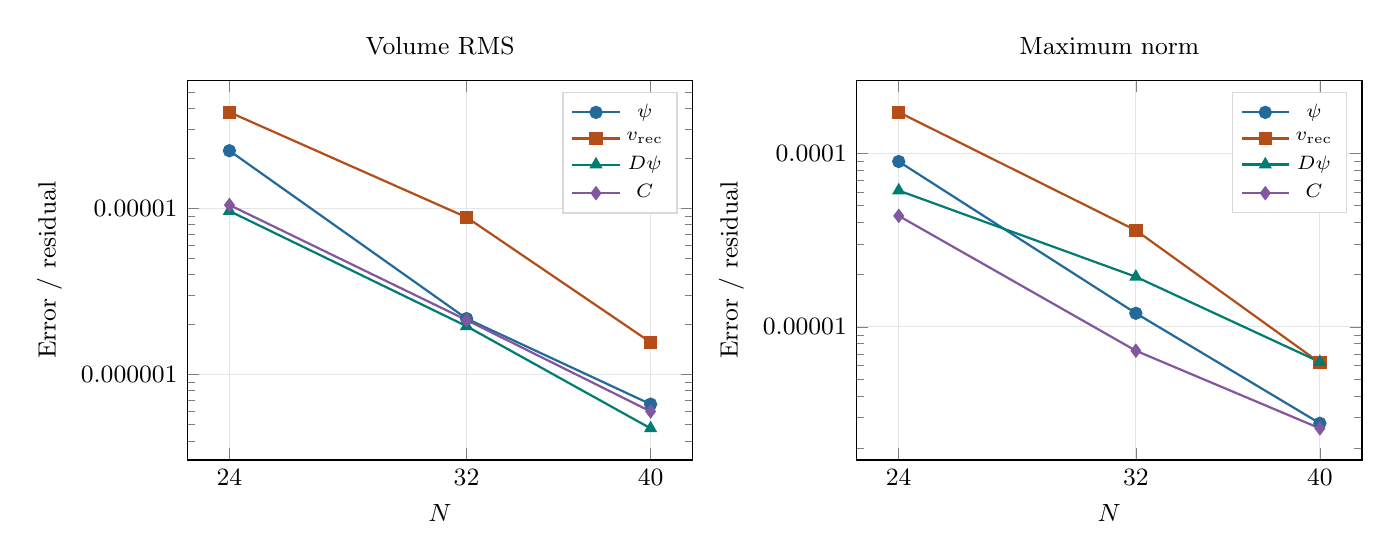
\begin{tikzpicture}
\begin{axis}[width=8cm,height=6.4cm,xmode=log,ymode=log,log ticks with fixed point,xtick={24,32,40},xlabel={$N$},ylabel={Error / residual},legend pos=north east,title={Volume RMS}]
\addplot[blue,mark=*,thick] coordinates {(24,2.21904628616e-05) (32,2.17197803105e-06) (40,6.64430969424e-07)};
\addlegendentry{$\psi$}
\addplot[bad,mark=square*,thick] coordinates {(24,3.78282525726e-05) (32,8.82809336563e-06) (40,1.564097913e-06)};
\addlegendentry{$v_{\rm rec}$}
\addplot[good,mark=triangle*,thick] coordinates {(24,9.62925965845e-06) (32,1.95459220767e-06) (40,4.75257653411e-07)};
\addlegendentry{$D\psi$}
\addplot[purple,mark=diamond*,thick] coordinates {(24,1.04719034e-05) (32,2.12857908637e-06) (40,6.00958068595e-07)};
\addlegendentry{$C$}
\end{axis}
\begin{axis}[at={(8.5cm,0)},anchor=south west,width=8cm,height=6.4cm,xmode=log,ymode=log,log ticks with fixed point,xtick={24,32,40},xlabel={$N$},ylabel={Error / residual},legend pos=north east,title={Maximum norm}]
\addplot[blue,mark=*,thick] coordinates {(24,8.96911316694e-05) (32,1.1984819866e-05) (40,2.78357661563e-06)};
\addlegendentry{$\psi$}
\addplot[bad,mark=square*,thick] coordinates {(24,0.000172568326764) (32,3.60207543337e-05) (40,6.21271036065e-06)};
\addlegendentry{$v_{\rm rec}$}
\addplot[good,mark=triangle*,thick] coordinates {(24,6.10508026456e-05) (32,1.94408275049e-05) (40,6.27548937074e-06)};
\addlegendentry{$D\psi$}
\addplot[purple,mark=diamond*,thick] coordinates {(24,4.36308979571e-05) (32,7.2919520825e-06) (40,2.60342537957e-06)};
\addlegendentry{$C$}
\end{axis}
\end{tikzpicture}\end{center}

\captionof{figure}{Corrected-source Minkowski errors at $t=12$ against the analytic angular wave, $N=24,32,40$. Both field derivatives and the independently measured reduction residual decrease. The full admission also includes the earlier times and separate bulk/shell checks; the minimum pair order across all of them is $3.64881$.}

\begin{center}\small
\begin{tabularx}{\linewidth}{@{}Xr@{}}\toprule
Measured quantity & Value \\\midrule
Minimum field/velocity/gradient/reduction pair order & $3.64881$ \\
Minimum actual compiled $\psi_t$ pair order & $3.833$ \\
Finest normalized reduction maximum & $1.1993\times10^{-3}$ \\
Maximum timestep fraction & $5.157\times10^{-7}$ \\
Maximum quarter/half difference ratio & $0.06769$ \\
Finite-cap waveform differences, $0.9S$, $0.95S$ & $1.254\times10^{-5}$, $7.580\times10^{-6}$ \\
Coarse $t=100$ late peak / initial peak & $8.723\times10^{-4}$ \\
Maximum scaled CPU/GPU field/derivative difference & $4.346\times10^{-14}$ \\\bottomrule
\end{tabularx}
\end{center}

Aurora job \texttt{8937736} validates the corrected configuration on an Intel Data Center GPU Max 1550 using SYCL. Its three-resolution fields are compared directly with the analytic wave and matching CPU trajectories. The $t=100$ flat-space stability run is a separate coarse control; the three fine CPU/GPU convergence trajectories end at $t=12$.

\textbf{A corrected evaluation defect matters.} An earlier smooth-layer evaluation formed $W(1-W)$ by subtracting a rounded $W$ from one. Near the layer endpoint, CPU/GPU shift gradients differed by about $0.01338$, and a strict evolved-field comparison failed at $1.85\times10^{-4}$. The corrected evaluator computes $W(1-W)=ab/(a+b)^2$, with $a=e^{-1/z}$ and $b=e^{-1/(1-z)}$, and differentiates the quotient without that cancellation. It changes no continuous map or physical background. The original reference stays bitwise unchanged. Earlier affected admissions are superseded, not erased.

\clearpage
\section{Results: completed Schwarzschild families still fail a gate}
The fixed actual excision cube has halfwidth $0.25M$. The following matrices use the corrected undamped operator. Matching completed trajectories are reused.
\begin{center}\small
\begin{tabularx}{\linewidth}{@{}p{2.5cm}X@{}}\toprule
Family & Outcome \\\midrule
$24,36,48$ & Late coarse-pair maximum-norm orders fail: velocity $1.441$, gradient $0.611$, reduction $0.685$. The $36/48$ pair passes. \\
$36,48,60$ & After resolving profile interpolation and independent-reference uncertainty, the remaining failure is $\psi$ volume-RMS order at $100M$: $p_{48,60}=1.40169<1.5$. \\
$24,48,96$ & Separately declared dyadic family. Early $2/6/12M$ checks pass. Fine evolution and full controls are unfinished. It does not retroactively change either failed matrix. \\\bottomrule
\end{tabularx}\end{center}
\begin{center}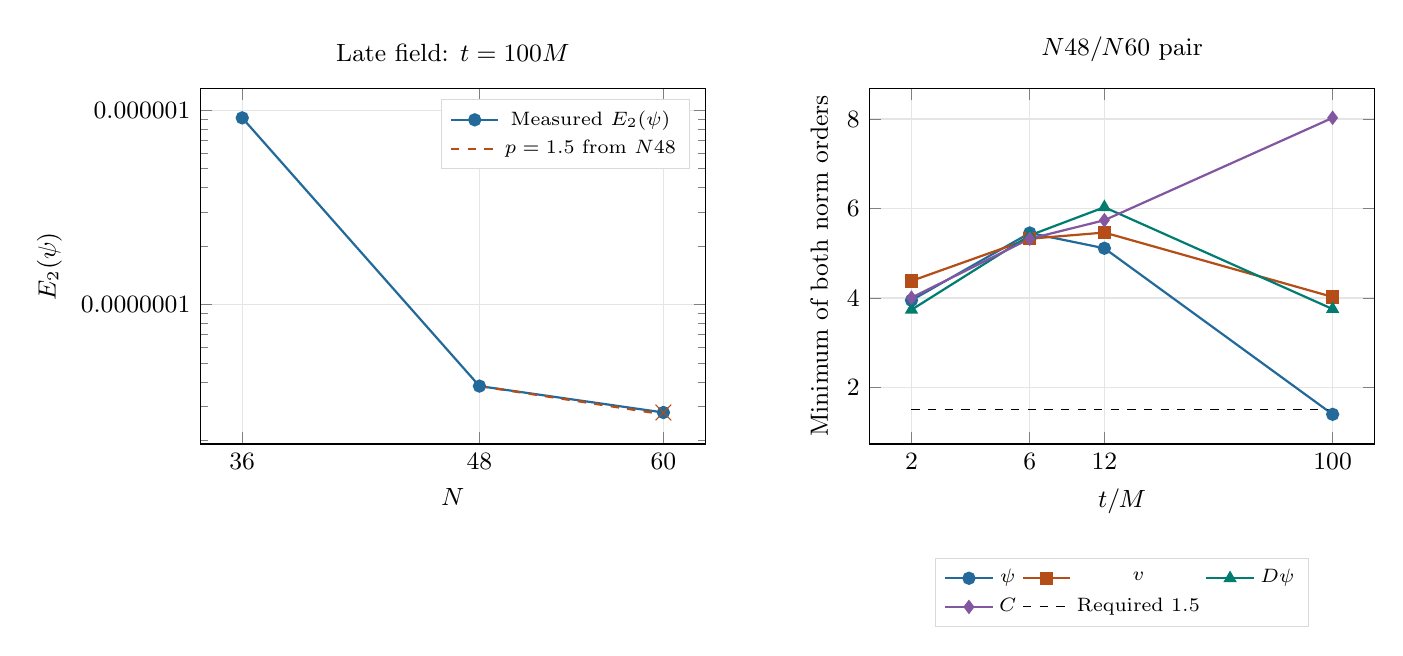
\begin{tikzpicture}
\begin{axis}[width=8cm,height=6.1cm,xmode=log,ymode=log,log ticks with fixed point,xtick={36,48,60},xlabel={$N$},ylabel={$E_2(\psi)$},title={Late field: $t=100M$},legend pos=north east]
\addplot[blue,thick,mark=*] coordinates {(36,9.12727653438e-07) (48,3.80574711139e-08) (60,2.78356801246e-08)};
\addlegendentry{Measured $E_2(\psi)$}
\addplot[bad,dashed,thick] coordinates {(48,3.80574711139e-08) (60,2.7231709588e-08)};
\addlegendentry{$p=1.5$ from $N48$}
\addplot[bad,only marks,mark=x,mark size=4pt] coordinates {(60,2.78356801246e-08)};
\end{axis}
\begin{axis}[at={(8.5cm,0)},anchor=south west,width=8cm,height=6.1cm,xmode=log,xtick={2,6,12,100},log ticks with fixed point,xlabel={$t/M$},ylabel={Minimum of both norm orders},title={$N48/N60$ pair},legend style={at={(.5,-.32)},anchor=north,legend columns=3}]
\addplot[blue,mark=*,thick] coordinates {(2,3.9490400771) (6,5.45330485885) (12,5.11162728071) (100,1.401693025)};
\addlegendentry{$\psi$}
\addplot[bad,mark=square*,thick] coordinates {(2,4.38246821645) (6,5.32423252713) (12,5.46293701822) (100,4.02410208849)};
\addlegendentry{$v$}
\addplot[good,mark=triangle*,thick] coordinates {(2,3.73730969689) (6,5.39917969262) (12,6.02854656613) (100,3.75328111086)};
\addlegendentry{$D\psi$}
\addplot[purple,mark=diamond*,thick] coordinates {(2,4.00737239816) (6,5.32415981116) (12,5.73804261838) (100,8.02556675521)};
\addlegendentry{$C$}
\addplot[black,dashed] coordinates {(2,1.5) (100,1.5)};
\addlegendentry{Required $1.5$}
\end{axis}
\end{tikzpicture}\end{center}

\captionof{figure}{Completed $36/48/60$ family using the resolved 2400-point independent reference and six-point sampling. Left: late field RMS error. Right: the minimum of the two norm orders for each quantity on the $48/60$ pair. The field at $100M$ falls below the declared order threshold. Errors decrease, so this is a failure of the required convergence rate, not evidence of error growth or a proof of inconsistency.}

At $100M$, the field RMS errors are
\begin{equation}
 E_{36}=9.12728\times10^{-7},\qquad E_{48}=3.80575\times10^{-8},\qquad
 E_{60}=2.78357\times10^{-8}.
\end{equation}
The coarse pair gives $p=11.045$, followed by $1.402$. That variation does not demonstrate an asymptotic regime. The actual compiled time-derivative audit passes with minimum order $2.791$, and the finest waveform/QNM/reduction-amplitude checks pass. The late field gate remains unresolved; its cause has not been established.

\clearpage
\subsection{Reference sampling, refinement and free-frequency fits}
PCHIP sampling introduced two early maximum-norm measurement failures when errors became very small. An independent polynomial and smooth-function instrument verified sixth-order local interpolation; reevaluating the same saved states with six-point sampling removed those early failures. The remaining late field order did not pass. Refining the reference from 1200 to 2400 points bounded its uncertainty by $2.08\%$ of the finest errors for the completed $36/48/60$ family.

The new $N96$ grid exposed a stricter reference requirement: at $2M$, the 1200/2400 velocity-reference difference was $13.80\%$ of the primary error, exceeding the unchanged $10\%$ bound. Only the independent oracle was refined to 4800 points. The 2400/4800 maximum early uncertainty is now $0.860\%$. No primary state was rerun or changed for this measurement.

The scalar target is $M\omega=0.4836438722-0.0967587760i$ \cite{qnm}. With $\omega=\omega_R-i\Gamma$, a Schwarzschild fit is
\begin{equation}
 z(t)\simeq e^{-\Gamma(t-t_0)}\left[A\cos\omega_R(t-t_0)+B\sin\omega_R(t-t_0)\right].
\end{equation}
Frequencies and amplitudes are fitted freely by multi-start variable projection; the independent target is used only for evaluation. Windows are $[35,65]$, $[40,70]$, $[45,75]M$. Kerr will use two free complex branches,
\begin{equation}
 z(t)\simeq A_+e^{-i\omega_+(t-t_0)}+A_-e^{-i\omega_-(t-t_0)},
\end{equation}
with both amplitudes and frequencies free. The negative-frequency branch is compared with the symmetry-related $m=-2$ scalar target; it is not silently discarded from real initial data.
\begin{center}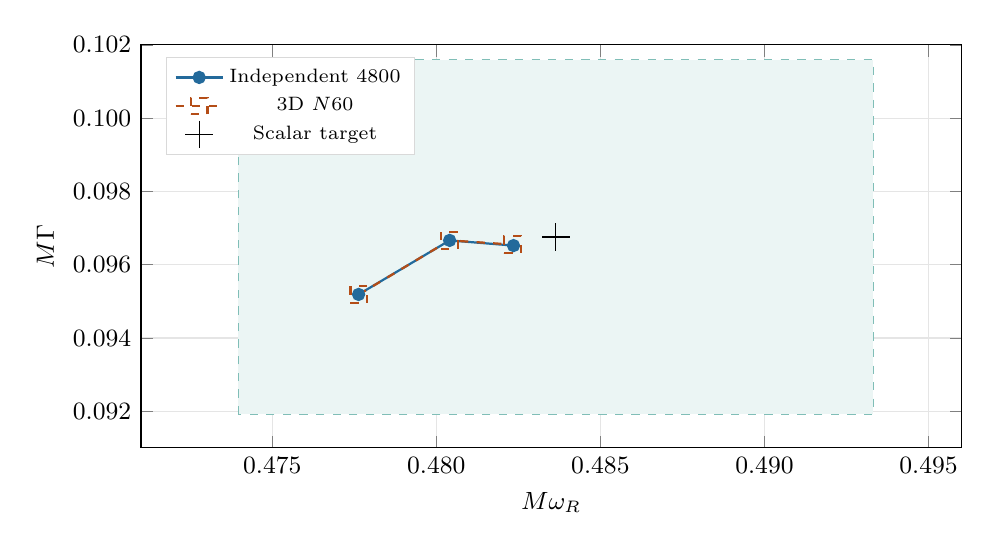
\begin{tikzpicture}
\begin{axis}[width=12cm,height=6.7cm,xlabel={$M\omega_R$},ylabel={$M\Gamma$},xmin=.471,xmax=.496,ymin=.091,ymax=.102,scaled ticks=false,xtick={.475,.480,.485,.490,.495},ytick={.092,.094,.096,.098,.100,.102},xticklabel style={/pgf/number format/fixed,/pgf/number format/precision=3,/pgf/number format/fixed zerofill},yticklabel style={/pgf/number format/fixed,/pgf/number format/precision=3,/pgf/number format/fixed zerofill},legend pos=north west]
\path[fill=good!8,draw=good!50,dashed] (axis cs:0.4739709947664984,0.09192083717937317) rectangle (axis cs:0.4933167496549269,0.10159671477720193);
\addplot[blue,mark=*,thick] coordinates {(0.477630638419,0.0951897921074) (0.48040537965,0.0966646309896) (0.482351640671,0.0965228920359)};
\addlegendentry{Independent 4800}
\addplot[bad,dashed,mark=square,mark size=3pt,thick] coordinates {(0.477635637676,0.0951853879762) (0.480400011263,0.0966653927717) (0.482324363161,0.0965506252927)};
\addlegendentry{3D $N60$}
\addplot[black,only marks,mark=+,mark size=5pt] coordinates {(0.483643872211,0.0967587759783)};
\addlegendentry{Scalar target}
\end{axis}
\end{tikzpicture}\end{center}
\captionof{figure}{Free Schwarzschild ringdown fits from the independent 4800-point reference and the completed 3D $N60$ trajectory. The rectangle is the declared $2\%$ real-frequency and $5\%$ decay tolerance; the cross is the independent spin-zero Leaver target. These fits pass, while the separate late spatial field-convergence gate still fails.}

\clearpage
\subsection{Unfinished dyadic family: what is already measured}
The $24/48/96$ family doubles every logical resolution and keeps the actual excision cube commensurate. The new $N96$ trajectory uses the same preserved CPU executable and scalar parameters as the reused $N24$ and $N48$ cases. The first five collected allocations close at $13,26,39,52,65M$ with identical physical/reference and derivative fingerprints.
\begin{center}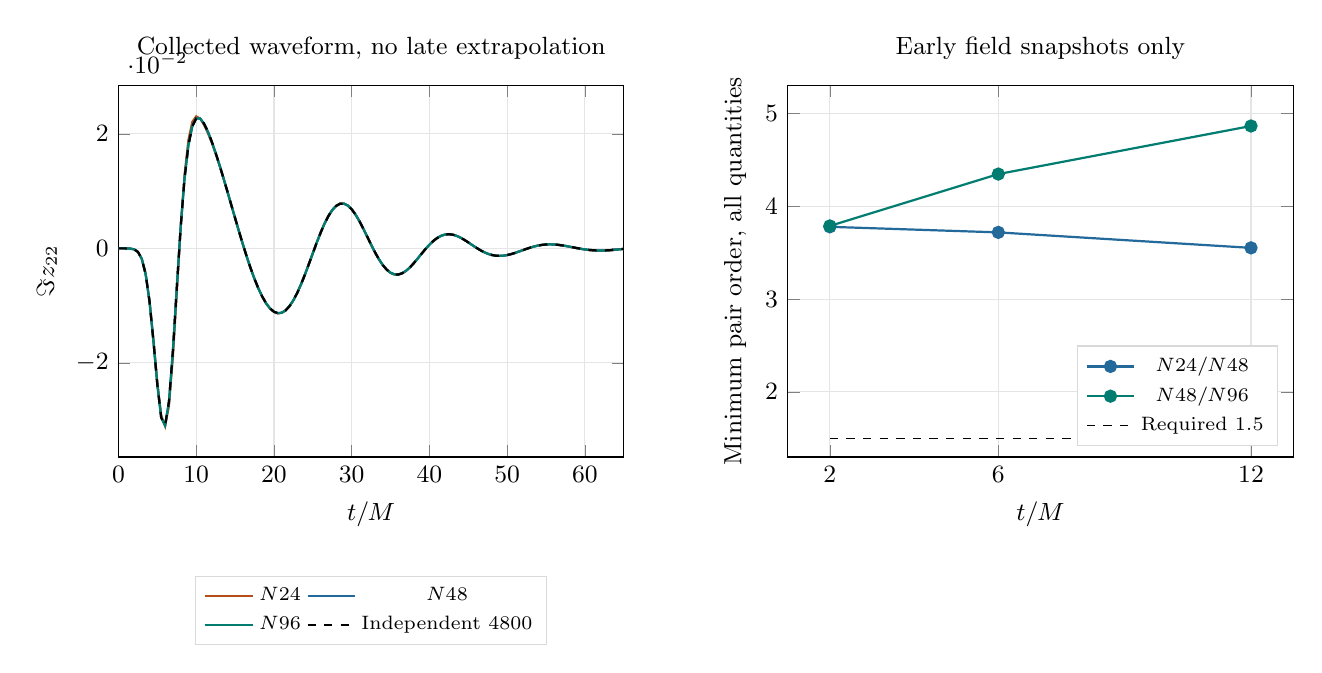
\begin{tikzpicture}
\begin{axis}[width=8cm,height=6.3cm,xlabel={$t/M$},ylabel={$\Im z_{22}$},xmin=0,xmax=65.0,title={Collected waveform, no late extrapolation},legend style={at={(.5,-.32)},anchor=north,legend columns=2}]
\addplot[bad,thick] coordinates {(0,-2.83998529903e-07) (0.5,-1.14340338918e-06) (1,-7.24156337223e-06) (1.5,-3.7806127721e-05) (2,-0.000167137682938) (2.5,-0.000612503485327) (3,-0.0018356045231) (3.5,-0.00451932800958) (4,-0.00925301463919) (4.5,-0.0159505738274) (5,-0.0233643717649) (5.5,-0.0292013634871) (6,-0.0310183604031) (6.5,-0.027452376367) (7,-0.0189869487467) (7.5,-0.0077359984528) (8,0.00358171586851) (8.5,0.0127941239282) (9,0.0189136187166) (9.5,0.0220771712908) (10,0.0230482634503) (10.5,0.0226805660064) (11,0.0216012002397) (11.5,0.0201474445984) (12,0.0184521043214) (12.5,0.0165570722819) (13,0.0144882228078) (13.5,0.0122821727468) (14,0.00998443158492) (14.5,0.00764032816926) (15,0.00528989206466) (15.5,0.00296817257603) (16,0.000708091825088) (16.5,-0.00145706723668) (17,-0.00349275123536) (17.5,-0.00536361875587) (18,-0.00703472172482) (18.5,-0.00847282155484) (19,-0.00964759340803) (19.5,-0.0105327117524) (20,-0.0111069124448) (20.5,-0.0113551205724) (21,-0.01126965939) (21.5,-0.0108514600828) (22,-0.0101111283774) (22.5,-0.0090697201289) (23,-0.00775911149858) (23.5,-0.00622187668731) (24,-0.00451059352979) (24.5,-0.00268650860901) (25,-0.000817532787749) (25.5,0.00102439938506) (26,0.00276650631193) (26.5,0.00433870922485) (27,0.00567733159756) (27.5,0.00672867509517) (28,0.00745218653846) (28.5,0.00782296562411) (29,0.0078334203663) (29.5,0.00749392283388) (30,0.00683235994597) (30.5,0.00589255245996) (31,0.00473163523766) (31.5,0.00341660450037) (32,0.00202029922009) (32.5,0.000617101945635) (33,-0.00072135126439) (33.5,-0.00193016726937) (34,-0.00295464258015) (34.5,-0.00375295520161) (35,-0.00429795486029) (35.5,-0.0045779669755) (36,-0.0045965992657) (36.5,-0.00437162230719) (37,-0.00393306632377) (37.5,-0.00332071660227) (38,-0.00258120011589) (38.5,-0.00176485485289) (39,-0.000922576637705) (39.5,-0.000102841680805) (40,0.000650911128236) (40.5,0.00130239446011) (41,0.00182399410776) (41.5,0.00219766008402) (42,0.00241517196501) (42.5,0.00247781830314) (43,0.00239555584996) (43.5,0.0021857312209) (44,0.00187146529859) (44.5,0.00147982492264) (45,0.00103992284713) (45.5,0.000581076066723) (46,0.000131119633849) (46.5,-0.000285055321303) (47,-0.00064668100444) (47.5,-0.000937957973374) (48,-0.0011485344514) (48.5,-0.00127362087313) (49,-0.00131376963561) (49.5,-0.00127436783511) (50,-0.00116489981375) (50.5,-0.000998040870688) (51,-0.000788645572533) (51.5,-0.000552695271744) (52,-0.00030626994475) (52.5,-6.46061983668e-05) (53,0.000158707357792) (53.5,0.000352363075135) (54,0.000507778397019) (54.5,0.000619346289846) (55,0.000684495061211) (55.5,0.000703568325184) (56,0.000679545537155) (56.5,0.000617633360392) (57,0.000524764815793) (57.5,0.000409045191467) (58,0.000279181826413) (58.5,0.000143930779926) (59,1.15886887136e-05) (59.5,-0.000110446028073) (60,-0.000216022302034) (60.5,-0.000300481053007) (61,-0.000360789008159) (61.5,-0.000395565271031) (62,-0.000405011708463) (62.5,-0.000390761366292) (63,-0.000355659783198) (63.5,-0.000303495443326) (64,-0.00023869845533) (64.5,-0.000166028747272) (65,-9.02744067119e-05)};
\addlegendentry{$N24$}
\addplot[blue,thick] coordinates {(0,-1.97034638567e-07) (0.5,-9.62632199439e-07) (1,-6.86310112246e-06) (1.5,-3.8021227433e-05) (2,-0.000168430936198) (2.5,-0.000608837679047) (3,-0.00181469469171) (3.5,-0.0044929339816) (4,-0.00929997018075) (4.5,-0.0161849617324) (5,-0.0237831803646) (5.5,-0.0295551638375) (6,-0.0309297127059) (6.5,-0.0267607634409) (7,-0.0179794622581) (7.5,-0.00698289321474) (8,0.00365359523702) (8.5,0.0121924446548) (9,0.0180111435138) (9.5,0.0213105172806) (10,0.0226618581239) (10.5,0.0226686064118) (11,0.021808084106) (11.5,0.0204029090971) (12,0.0186520605171) (12.5,0.016674050626) (13,0.0145414232371) (13.5,0.0123028236721) (14,0.00999557530351) (14.5,0.00765243075034) (15,0.00530503570494) (15.5,0.00298556282334) (16,0.000727309990286) (16.5,-0.00143534253153) (17,-0.00346738218965) (17.5,-0.00533380964529) (18,-0.00700042150638) (18.5,-0.00843473287605) (19,-0.00960697421312) (19.5,-0.0104911431685) (20,-0.01106613833) (20.5,-0.0113169631814) (21,-0.0112359501391) (21.5,-0.0108239362609) (22,-0.0100913003202) (22.5,-0.00905874909841) (23,-0.0077577315816) (23.5,-0.0062303642257) (24,-0.00452876769492) (24.5,-0.00271374820066) (25,-0.000852804216753) (25.5,0.000982502540549) (26,0.00271970874212) (26.5,0.0042889772874) (27,0.00562677189513) (27.5,0.00667942104822) (28,0.00740629756779) (28.5,0.00778235313001) (29,0.00779978641296) (29.5,0.00746868343516) (30,0.00681654872942) (30.5,0.00588673666039) (31,0.00473587953173) (31.5,0.00343048944671) (32,0.00204297694305) (32.5,0.000647369615348) (33,-0.000684971037948) (33.5,-0.00188934294034) (34,-0.00291114669534) (34.5,-0.00370857103821) (35,-0.00425437670041) (35.5,-0.00453670494255) (36,-0.00455890861915) (36.5,-0.00433847048717) (37,-0.00390513161919) (37.5,-0.0032983980209) (38,-0.00256462218516) (38.5,-0.00175386981326) (39,-0.000916780763027) (39.5,-0.00010161796543) (40,0.000648328424005) (40.5,0.00129685001844) (41,0.00181635225448) (41.5,0.00218876233126) (42,0.0024058073292) (42.5,0.00246869605957) (43,0.00238727265369) (43.5,0.00217873584999) (44,0.00186603578792) (44.5,0.0014760700906) (45,0.001037802371) (45.5,0.000580420732693) (46,0.000131641521657) (46.5,-0.000283755186551) (47,-0.00064509332391) (47.5,-0.000936629039753) (48,-0.00114802036053) (48.5,-0.00127444274395) (49,-0.00131637549138) (49.5,-0.00127910054735) (50,-0.00117196812165) (50.5,-0.00100749270459) (51,-0.000800347405561) (51.5,-0.000566324096066) (52,-0.00032132264345) (52.5,-8.04251522631e-05) (53,0.000142898824051) (53.5,0.000337421764089) (54,0.00049460081971) (54.5,0.000608825151211) (55,0.000677471540687) (55.5,0.000700782417802) (56,0.000681589427354) (56.5,0.00062491271894) (57,0.000537470666967) (57.5,0.000427136568959) (58,0.000302378452199) (58.5,0.000171715919948) (59,4.32239887829e-05) (59.5,-7.58917214617e-05) (60,-0.00017963052685) (60.5,-0.000263431810138) (61,-0.000324305412369) (61.5,-0.000360859326864) (62,-0.000373232521958) (62.5,-0.000362945649575) (63,-0.000332685890663) (63.5,-0.000286044301763) (64,-0.000227225153805) (64.5,-0.000160746733256) (65,-9.11517125538e-05)};
\addlegendentry{$N48$}
\addplot[good,thick] coordinates {(0,-1.95410167318e-07) (0.5,-9.64200216234e-07) (1,-6.87002289999e-06) (1.5,-3.79998249337e-05) (2,-0.000168194333905) (2.5,-0.000607994625016) (3,-0.0018134224592) (3.5,-0.00449357686305) (4,-0.00930660154063) (4.5,-0.0161975157769) (5,-0.0237916987335) (5.5,-0.0295465841781) (6,-0.0309045549035) (6.5,-0.0267371263961) (7,-0.0179749769935) (7.5,-0.00699705773406) (8,0.00363519855593) (8.5,0.0121815105104) (9,0.018008931659) (9.5,0.0213126568378) (10,0.0226648122202) (10.5,0.022671274344) (11,0.0218105173393) (11.5,0.0204052518829) (12,0.018654219581) (12.5,0.0166756043765) (13,0.0145416987624) (13.5,0.0123012061944) (14,0.00999187858346) (14.5,0.0076470861894) (15,0.00529901097219) (15.5,0.00298008362963) (16,0.000723514646757) (16.5,-0.00143666559804) (17,-0.003465955473) (17.5,-0.0053298678712) (18,-0.00699461068166) (18.5,-0.00842796485796) (19,-0.00960024467406) (19.5,-0.0104853630125) (20,-0.0110620006111) (20.5,-0.0113148574004) (21,-0.011235935834) (21.5,-0.0108257758238) (22,-0.0100945367313) (22.5,-0.00906280705289) (23,-0.00776201940658) (23.5,-0.00623435770703) (24,-0.00453206492542) (24.5,-0.00271609346218) (25,-0.000854085532621) (25.5,0.000982273896471) (26,0.00272042803902) (26.5,0.00429047841056) (27,0.00562885648709) (27.5,0.00668188172323) (28,0.00740893536126) (28.5,0.00778499018457) (29,0.00780227402079) (29.5,0.0074709063557) (30,0.00681842690094) (30.5,0.00588822414758) (31,0.00473696116914) (31.5,0.00343117642247) (32,0.00204330127165) (32.5,0.000647377458295) (33,-0.000685225842112) (33.5,-0.00188980435461) (34,-0.00291176136912) (34.5,-0.00370929245964) (35,-0.00425516790186) (35.5,-0.00453753939678) (36,-0.004559769386) (36.5,-0.00433934829454) (37,-0.00390602260088) (37.5,-0.00329930106296) (38,-0.00256553595254) (38.5,-0.00175478991021) (39,-0.000917697527565) (39.5,-0.000102515250559) (40,0.000647473513393) (40.5,0.00129606668219) (41,0.00181567471423) (41.5,0.00218822734262) (42,0.0024054508096) (42.5,0.00246854959202) (43,0.00238736008369) (43.5,0.0021790700815) (44,0.00186661607536) (44.5,0.00147688017591) (45,0.00103881002103) (45.5,0.000581578862196) (46,0.000132890415429) (46.5,-0.000282484692075) (47,-0.000643875379017) (47.5,-0.000935537303583) (48,-0.00114712234125) (48.5,-0.00127379454289) (49,-0.0013160171595) (49.5,-0.00127905237942) (50,-0.00117222844944) (50.5,-0.00100803754198) (51,-0.000801131906934) (51.5,-0.000567285662554) (52,-0.000322385469286) (52.5,-8.15059222315e-05) (53,0.000141884468692) (53.5,0.000336552604466) (54,0.000493943991276) (54.5,0.000608431102165) (55,0.000677370271864) (55.5,0.000700981298621) (56,0.000682072882398) (56.5,0.000625643834992) (57,0.000538394460732) (57.5,0.000428184537597) (58,0.000303474076432) (58.5,0.000172780723265) (59,4.41835995295e-05) (59.5,-7.51020366286e-05) (60,-0.000179061270797) (60.5,-0.000263115891438) (61,-0.00032425617772) (61.5,-0.000361070122127) (62,-0.000373677830982) (62.5,-0.000363583606075) (63,-0.0003334618097) (63.5,-0.000286894958074) (64,-0.00022808354721) (64.5,-0.000161546949474) (65,-9.1833459454e-05)};
\addlegendentry{$N96$}
\addplot[black,dashed,thick] coordinates {(0,-1.95383504623e-07) (0.5,-9.64234961315e-07) (1,-6.8701255258e-06) (1.5,-3.79990265815e-05) (2,-0.000168188534048) (2.5,-0.000607978462547) (3,-0.00181340692788) (3.5,-0.00449360918331) (4,-0.0093067311427) (4.5,-0.0161976933704) (5,-0.0237917533735) (5.5,-0.0295463956685) (6,-0.030904233268) (6.5,-0.026736924918) (7,-0.0179750305796) (7.5,-0.0069972781068) (8,0.00363498789183) (8.5,0.0121814098062) (9,0.0180089316422) (9.5,0.0213127013506) (10,0.0226648573798) (10.5,0.0226713056833) (11,0.0218105418581) (11.5,0.0204052861054) (12,0.0186542791871) (12.5,0.0166756919312) (13,0.0145417918089) (13.5,0.0123012554877) (14,0.009991826567) (14.5,0.00764690225637) (15,0.00529872381728) (15.5,0.00297978513583) (16,0.000723325334836) (16.5,-0.00143665376706) (17,-0.00346572993896) (17.5,-0.00532950369147) (18,-0.00699423925978) (18.5,-0.00842771481292) (19,-0.00960018951349) (19.5,-0.0104854980052) (20,-0.0110622553326) (20.5,-0.0113151324789) (21,-0.0112361439172) (21.5,-0.0108258695903) (22,-0.0100945160313) (22.5,-0.00906270758343) (23,-0.00776189180272) (23.5,-0.00623424702632) (24,-0.00453199755872) (24.5,-0.00271607385281) (25,-0.000854100959216) (25.5,0.00098224441685) (26,0.00272040476232) (26.5,0.00429047469172) (27,0.00562887651612) (27.5,0.00668192169475) (28,0.00740898667774) (28.5,0.00778504313556) (29,0.00780232071825) (29.5,0.00747094231132) (30,0.00681845123149) (30.5,0.00588823872596) (31,0.00473696925903) (31.5,0.00343118134843) (32,0.00204330542754) (32.5,0.000647381792614) (33,-0.000685221792401) (33.5,-0.00188980204023) (34,-0.00291176266019) (34.5,-0.00370929911914) (35,-0.00425518120482) (35.5,-0.00453755990117) (36,-0.00455979688192) (36.5,-0.00433938192196) (37,-0.00390606103187) (37.5,-0.00329934268691) (38,-0.00256557904851) (38.5,-0.00175483281013) (39,-0.000917738717871) (39.5,-0.000102553442724) (40,0.000647439358073) (40.5,0.00129603738653) (41,0.00181565092951) (41.5,0.00218820957418) (42,0.00240543941601) (42.5,0.00246854476852) (43,0.00238736184751) (43.5,0.00217907824053) (44,0.00186663021118) (44.5,0.00147689965632) (45,0.00103883402618) (45.5,0.000581606415478) (46,0.000132920418685) (46.5,-0.000282453412646) (47,-0.000643844019276) (47.5,-0.00093550702084) (48,-0.00114709418792) (48.5,-0.00127376941131) (49,-0.00131599573982) (49.5,-0.00127903512066) (50,-0.00117221553922) (50.5,-0.00100802891742) (51,-0.000801127289206) (51.5,-0.000567284600326) (52,-0.000322387387155) (52.5,-8.15101787173e-05) (53,0.00014187852404) (53.5,0.000336545584867) (54,0.000493936435195) (54.5,0.00060842343984) (55,0.000677362805919) (55.5,0.000700974196223) (56,0.000682066179153) (56.5,0.000625637454187) (57,0.000538388239245) (57.5,0.000428178253617) (58,0.000303467479976) (58.5,0.00017277356761) (59,4.41756716513e-05) (59.5,-7.51108937047e-05) (60,-0.000179071138569) (60.5,-0.000263126757875) (61,-0.000324267925902) (61.5,-0.00036108252768) (62,-0.000373690567312) (62.5,-0.000363596255443) (63,-0.000333473879852) (63.5,-0.000286905903424) (64,-0.000228092793624) (64.5,-0.000161553923808) (65,-9.18376215856e-05)};
\addlegendentry{Independent 4800}
\end{axis}
\begin{axis}[at={(8.5cm,0)},anchor=south west,width=8cm,height=6.3cm,xlabel={$t/M$},ylabel={Minimum pair order, all quantities},xtick={2,6,12},ymin=1.3,ymax=5.3,title={Early field snapshots only},legend pos=south east]
\addplot[blue,thick,mark=*] coordinates {(2,3.77778769137) (6,3.71779131351) (12,3.55114919787)};
\addlegendentry{$N24/N48$}
\addplot[good,thick,mark=*] coordinates {(2,3.78737995584) (6,4.34557491236) (12,4.8632468925)};
\addlegendentry{$N48/N96$}
\addplot[black,dashed] coordinates {(2,1.5) (12,1.5)};
\addlegendentry{Required $1.5$}
\end{axis}
\end{tikzpicture}\end{center}

\captionof{figure}{Collected dyadic evidence only. Left: the extracted waveform through $65M$, with the independently resolved reference. Right: minimum pair orders over field, coordinate velocity, independent gradient and reduction, both norms, at the three available field-comparison times. There is no $100M$ point for $N96$; no late order is inferred or plotted.}

\begin{center}\small
\begin{tabularx}{\linewidth}{@{}Xr@{}}\toprule
Partial diagnostic & Measured value \\\midrule
Minimum early pair order & $3.55115$ \\
Largest 2400/4800 reference difference / finest error & $0.0085991$ \\
Independent waveform relative L2 error through $65M$ & $1.153\times10^{-5}$ \\
Maximum normalized reduction through collected reports & $0.00041615$ \\\bottomrule
\end{tabularx}\end{center}

These indicators pass their corresponding partial checks. The missing late field comparison is precisely the test that failed in the preceding completed family, so early success cannot settle it. The final reference-uncertainty certificate, actual compiled derivative audit, half/quarter timesteps, inner-cube and outer-cap controls remain required before Schwarzschild CPU admission. Its GPU stage and all nonzero-spin Kerr evolution remain gated on that admission.

\clearpage
\section{Boundary reach, failed alternatives and present limitations}
\subsection{Finite caps do not test all late reflections}
Required caps are $\rho=0.9S$ and $0.95S$, compared with exact scri. For the chosen Schwarzschild chart, radial round-trip estimates to the extraction region are about $430M$ and $913M$. Agreement through $100M$ therefore does not establish immunity to reflections that can return later. A closer $0.6S$ supplement has a radial return estimate near $60.4M$ and is declared to report its late sensitivity, field errors and QNM behaviour separately. The largest sampled radial return time is not a universal upper bound for all null rays; angular motion and trapping can delay them.

\subsection{Failed or superseded methods are preserved}
\begin{center}\small
\begin{tabularx}{\linewidth}{@{}p{3.4cm}X@{}}\toprule
Attempt & What prevented promotion \\\midrule
Compatible discrete reduction & Small residuals were accompanied by field growth at the Cartesian/shell interface. Constraint control alone was insufficient. \\
Normal upwind with the earlier endpoint closure & Short tests passed, but long controls failed near $51$ flat-space time units and $62M$ in Schwarzschild. \\
Fixed or grid-scaled scalar damping matrices & Several late reduction-convergence orders missed $1.5$. No roundoff exemption was used. \\
Smooth-layer v21 coefficient evaluator & Independent endpoint audit and strict CPU/GPU agreement exposed a derivative-evaluation defect; source-bound admissions were superseded. \\
Schwarzschild $N36$, $\kappa=2$ diagnostic & Same initial data and frozen coefficients; late field RMS error became $2.2484$ times worse and QNM window consistency failed, despite a smaller reduction residual. \\\bottomrule
\end{tabularx}\end{center}

\subsection{What has not been demonstrated}
There is no global multipatch energy estimate, admitted Schwarzschild $100M$ three-resolution family with all controls, nonzero-spin Kerr ringdown result, validated near-extremal evolution, or late Price-tail study. Physical energy and angular-momentum balance diagnostics have not been established as part of these admissions. A read-only CPU memory-placement audit found bitwise identical full scalar RHS values, but HBM placement was slower ($63.8$ versus $43.7$ ms per fill/evaluate pair); it supplied no scientific admission and the default placement was retained.

All black-hole fields in this document are test fields on an exact stationary geometry. Their evolution cannot test gauge-driver stability, Einstein/Z4c constraints, nonlinear gravitational radiation, or scalar backreaction. Reusing the mesh and interpolation is useful numerical evidence, with that limited scope.

\clearpage
\section{Relationship to previous literature}
This is a validation experiment for an existing Cartesian-plus-shell infrastructure, not a claim of a new conformal scalar equation or the first fixed-background hyperboloidal Kerr evolution. The comparisons below concern the cited methods, not a reproduction of all their published results.

\begin{center}\small
\begin{tabularx}{\linewidth}{@{}p{3.0cm}X X@{}}\toprule
Work & Shared treatment & Present distinction \\\midrule
Zengino\u glu (2008) \cite{scrifixing} & Stationary height transformation and conformal compactification with scri at a fixed coordinate location. & The inner chart here is the selected analytic trumpet; the map is frozen, with a separate immutable Minkowski reference. \\
Zengino\u glu--Tiglio (2009) \cite{matching} & Fixed-Kerr massless scalar, actual conformal curvature, inner/outer matching, RK4 and direct access to scri. & Their angular pseudospectral and radial finite-difference treatment is replaced by full 3D Cartesian components on seven patches. The current radial closure is SBP $6/3$. \\
R\'acz--T\'oth (2011) \cite{tails} & Fixed Kerr, compactification, scalar ringing/tails, and convergence tests. & Their spherical-harmonic angular representation and imposed radial reduction contrast with our 3D evolved gradient auxiliaries and measured residuals. They also test energy/angular-momentum balances. \\
Dennison et al. (2014/2015) \cite{trumpet} & Their exact $R_0=M$ trumpet supplies the inner stationary geometry. & The outer hyperboloidal layer, its mass-dependent asymptotics, scalar evolution and seven-patch validation are additional construction. Their coordinate caveat remains relevant. \\
Panosso Macedo (2020) \cite{macedo} & Hyperboloidal Kerr geometry and regular spin-zero wave propagation; relation to independent mode calculations. & The present inner-trumpet-plus-layer coordinates are not the minimal gauge. We use explicit 3D time evolution, not a separated frequency-domain evolution. \\\bottomrule
\end{tabularx}\end{center}

The closest PDE comparison is \cite{matching}: its conformal and coordinate-based treatments are equivalent when the rescaling and maps are chosen consistently. Our use of $R[\G]/6$ follows that principle. Its reported matching errors also motivate testing the layer and patch interfaces instead of trusting formal bulk order. These notes do not transfer another method's stability or convergence evidence to the present interpolation.

The reduced angular approaches in \cite{tails,macedo} avoid evolving a full 3D grid for a single azimuthal mode. Here the extra cost deliberately exercises the reusable Cartesian bulk, six shell blocks and their transfers. The independent reduced solvers are therefore valuable precisely because they do not share those interfaces. This does not make their error negligible: their uncertainty is measured against the actual finest 3D errors.

\clearpage
\subsection{A useful literature diagnostic not yet completed here}
For the physical test field one may compute, without backreaction,
\begin{equation}
 T_{ab}[\Phi]=\partial_a\Phi\partial_b\Phi-\tfrac12g_{ab}\partial_c\Phi\partial^c\Phi,
 \qquad \nabla_aT^{ab}=0\quad\hbox{when }\Box_g\Phi=0.
\end{equation}
The stationary and axial Killing fields yield
\begin{equation}
 J_E^a=-T^a{}_b\xi^b,\qquad J_L^a=T^a{}_b\eta^b,\qquad
 \nabla_aJ_E^a=\nabla_aJ_L^a=0.
\end{equation}
Flux-balance checks of this kind would complement the present error and QNM diagnostics, as illustrated by \cite{tails}. They have not been implemented and passed as a complete budget here. Computing a stress tensor for diagnostics would still not source Einstein's equations.

\section{What remains, and how evidence is preserved}
The next scientific decision is the $N96$ field and derivative comparison at $100M$ against the selected resolved reference, with the unchanged $1.5$ gate. If it passes, the declared time, inner and outer controls and actual-RHS audit must also pass. Only then can the source-bound Schwarzschild CPU result authorize a short direct GPU validation. Kerr subsequently needs its own independent solution, three-resolution fields and derivatives, reference uncertainty, characteristic/boundary checks, free two-branch QNMs and matching GPU result.

Aurora submissions use \texttt{debug}, account \texttt{CompactBinaryMerger}, one node and at most 60 minutes, with at most one task allocation queued or running. Bounded native checkpoints continue the same trajectory, rather than repeat completed runs. Native scalar payloads, source and executable SHA256 hashes, scheduler records, checkpoint ancestry and plots are retained. Physical and reference coefficient caches, and their derivative caches, have four separate before/after fingerprints. External SHA256 manifests cover files.

The production protection manifest covers 642 original source/input files, including pre-existing user changes. The latest checked snapshot has zero mismatches. The standalone scalar code is confined to \epath{src/test_scalar}; diagnostics and controllers are under \epath{tst/test_scalar}. Its build does not link production Z4c state or tasks.

\boxnote{\textbf{Decision rule.} Preserve and report every failure. Refine an unresolved independent reference without repeating the primary trajectory. Do not replace a failed declared family with a favourable plot. Claim admission only for the exact source, settings and complete set of passed gates. Scalar admission never completes the metric-evolution goal.}

\clearpage
\appendix
\section{Independent radial equation and scalar QNM conventions}
For Schwarzschild write $\psi=P(t,\rho)Y_{\ell m}$. With $\bar\Sigma=(\rho+M\Omega)^2$ and $D_r=\lambda\bar\Sigma$, define
\begin{equation}
 B_r^t=D_r^{-1}\partial_\rho(D_r\G^{\rho t}),\qquad
 B_r^\rho=D_r^{-1}\partial_\rho(D_r\G^{\rho\rho}).
\end{equation}
The independent radial equation is
\begin{equation}
 \G^{tt}P_{tt}+2\G^{t\rho}P_{t\rho}+\G^{\rho\rho}P_{\rho\rho}
 +B_r^tP_t+B_r^\rho P_\rho
 -\left[V+\frac{\ell(\ell+1)}{\bar\Sigma}\right]P=0.
\end{equation}
Its separate normal-momentum implementation evolves $(P,\Pi_r,Q_\rho)$ on a uniform radial grid and includes its own scalar auxiliary damping. The latter vanishes on $Q_\rho=P_\rho$ and is independently resolution/time/inner-boundary controlled. No primary cached metric or multipatch RHS is imported.

For regular $m=2$ Kerr angular dependence,
\begin{equation}
 \Delta_{S^2}\{(1-z^2)W_2e^{2i\phi}\}
 =(1-z^2)e^{2i\phi}\{(1-z^2)W_{2,zz}-6zW_{2,z}-6W_2\}.
\end{equation}
Substitution into the full frozen operator, with $\partial_\phi\mapsto2i$, retains the exact Kerr radial-azimuthal cross terms. Factoring the polar zero makes the independent angular function regular; it does not discard angular mode coupling.

Independent frequency targets use spin-weight-zero separation in Boyer--Lindquist coordinates,
\begin{equation}
 \Phi=e^{-i\omega T_{\rm BL}}e^{im\phi_{\rm BL}}S_{\ell m}(\theta)\mathcal R(R),\qquad
 K_\omega=(R^2+a^2)\omega-am,
\end{equation}
\begin{align}
 \frac1{\sin\theta}\partial_\theta(\sin\theta\,\partial_\theta S)
 +\left(a^2\omega^2\cos^2\theta-\frac{m^2}{\sin^2\theta}+A_{\ell m}\right)S&=0,\\
 \partial_R(\Delta\partial_R\mathcal R)
 +\left[\frac{K_\omega^2}{\Delta}-a^2\omega^2+2am\omega-A_{\ell m}\right]\mathcal R&=0.
\end{align}
QNM conditions are ingoing at the future horizon and outgoing at infinity. With $\dd R_*/\dd R=(R^2+a^2)/\Delta$, $\Omega_H=a/(R_+^2+a^2)$, the leading radial factors are $e^{-i(\omega-m\Omega_H)R_*}$ at the horizon and $R^{-1}e^{+i\omega R_*}$ at infinity. Stationary radial time/azimuth transformations change those factors, not the Killing frequency. The \texttt{qnm} Leaver solver supplies the evaluation targets \cite{qnm}.

\clearpage
\section{Mode targets and evidence map}
\begin{center}\small
\begin{tabular}{@{}ccrr@{}}\toprule
$a/M$ & $(s,\ell,m,n)$ & $\Re(M\omega)$ & $-\Im(M\omega)$ \\\midrule
$0$ & $(0,2,2,0)$ & $0.483643872211$ & $0.096758775978$ \\
$0.5$ & $(0,2,2,0)$ & $0.585989629305$ & $0.093494418992$ \\
$0.5$ & $(0,2,-2,0)$ & $0.422751280000$ & $0.095615863282$ \\\bottomrule
\end{tabular}\end{center}
These are scalar frequencies. They are not spin-two gravitational ringdown frequencies. The Kerr values are targets, not measurements from an admitted Kerr run. The table lists positive-frequency solver targets; in an $m=2$ two-branch fit the symmetry-related branch is
\begin{equation}
 M\omega_-=-\big(M\omega_{s=0,\ell=2,m=-2,n=0}\big)^*
 =-0.422751280000-0.095615863282i.
\end{equation}

All evidence paths below are relative to \epath{docs/validation/test-scalar-20261016/}. Figure coordinates and reported numerical values are generated from the corresponding saved JSON/CSV files. The adjacent notes manifest binds the input hashes, generated source, generator and template. Figures are vector TikZ/PGFPlots embedded in the standalone \LaTeX{} source; no external images or bibliography files are required to compile it.

\begin{description}[style=nextline,font=\normalfont\bfseries]
\item[Current Minkowski admission] \epath{minkowski-stable-sbp-cpu-admission.json}; \epath{cpu-v22/stable-full-review.json}; \epath{aurora/minkowski-stable-gpu-v5-review.json}.
\item[Completed failed Schwarzschild matrices] \epath{cpu-schwarzschild-commensurate/primary-review.json}; \epath{cpu-schwarzschild-commensurate-finer/primary-resolved-reference-review.json}.
\item[Actual scalar time derivative] \epath{cpu-schwarzschild-commensurate-finer/actual-resolved-rhs-review.json}.
\item[Unfinished dyadic family] \epath{schwarzschild-dyadic-plan.json}; \epath{cpu-schwarzschild-dyadic/closed-prefix-t65-review.json}; \epath{cpu-schwarzschild-dyadic/reference-selection.json}.
\item[Verified continuation after access recovery] \epath{aurora/cpu-schwarzschild-dyadic-n96-resume5/submission.json}, job \texttt{8939561}; its parent is the verified $65M$ checkpoint.
\item[Independent QNM and reference checks] \epath{radial-oracle/smooth/qnm-n4800-review.json}; \epath{radial-oracle/smooth/resolved-reference-certificate-v1.json}; \epath{reference-interpolation-diagnostic-v1.json}.
\item[Protected baseline and access interruption] \epath{frozen-baseline-sha256.json}; \epath{access-recovery-20261017/status.json}; \epath{access-recovery-20261017/handoff.json}.
\end{description}

\begin{center}\small
\begin{tabular}{@{}ll@{}}\toprule
Current scalar source & SHA256 prefix (full digests in manifest) \\\midrule
\texttt{CMakeLists.txt} & \texttt{2e9a2a185016c799db00} \\
\texttt{main.cpp} & \texttt{87ae260c79c5af7f810f} \\
\texttt{geometry.hpp} & \texttt{0a29cae4c0588e406e20} \\
\texttt{sbp63.hpp} & \texttt{d99f847e559f5e93ac11} \\
\bottomrule\end{tabular}\end{center}
These notes are a dated evidence summary. Later resumed jobs may create additional results; the existing failure and admission records remain immutable.

\clearpage
\begin{thebibliography}{9}
\bibitem{scrifixing} A.~Zengino\u glu, \emph{Hyperboloidal foliations and scri-fixing} (2008), \href{https://arxiv.org/abs/0712.4333}{arXiv:0712.4333}. Stationary compactifications of Minkowski, Schwarzschild and Kerr.
\bibitem{matching} A.~Zengino\u glu and M.~Tiglio, \emph{Spacelike matching to null infinity} (2009), \href{https://arxiv.org/abs/0906.3342}{arXiv:0906.3342}. Fixed-background scalar equation, equivalent conformal/coordinate treatments and numerical matching tests; see Sections III--V.
\bibitem{tails} I.~R\'acz and G.~Zs.~T\'oth, \emph{Numerical investigation of the late-time Kerr tails} (2011), \href{https://arxiv.org/abs/1104.4199}{arXiv:1104.4199}. Angular spectral evolution, radial reduction and conservation diagnostics; see Section 2.
\bibitem{trumpet} K.~A.~Dennison, T.~W.~Baumgarte and P.~J.~Montero, \emph{Trumpet Slices in Kerr Spacetimes} (2014; revised 2015), \href{https://arxiv.org/abs/1409.1887}{arXiv:1409.1887}. Exact stationary trumpet family and the limiting-surface coordinate caveat.
\bibitem{macedo} R.~Panosso Macedo, \emph{Hyperboloidal framework for the Kerr spacetime} (2020), \href{https://arxiv.org/abs/1910.13452}{arXiv:1910.13452}. General Kerr hyperboloidal gauges, Teukolsky equations and minimal-gauge/frequency-domain connections.
\bibitem{qnm} L.~C.~Stein, \emph{qnm: A Python package for calculating Kerr quasinormal modes, separation constants, and spherical-spheroidal mixing coefficients} (2019), \href{https://arxiv.org/abs/1908.10377}{arXiv:1908.10377}, \href{https://doi.org/10.21105/joss.01683}{doi:10.21105/joss.01683}. The saved scalar targets use package version 0.4.4, spin weight $s=0$.
\end{thebibliography}
\end{document}
